%!TEX root = ../thesis.tex
\chapter{Results}
\label{ch:results}
This chapter is based on Figure~\ref{fig:Flowchart} and first discusses the comparison of \acrshort{abb} and \acrshort{obb} formats, then the permutation experiments to test robustness, and finally the ablation study to evaluate individual components.

In the image collages (see Fig. \ref{fig:aab_obb_example_pics}, \ref{fig:perm_exp_example_pics} and \ref{fig:ablation_example_pics}) use the colour scheme defined in Table \ref{tab:class_colors} to make the model predictions clearly distinguishable and to ensure unambiguous assignment to the respective classes.

\section{Oriented Bounding Boxes and Axis-aligned Bounding Boxes}
\todo{Bilder in Originalgröße in Appendix packen}
\begin{figure}[h]
    \centering
    
    % Erste Zeile
    \begin{subfigure}[b]{0.45\textwidth}
        \centering
        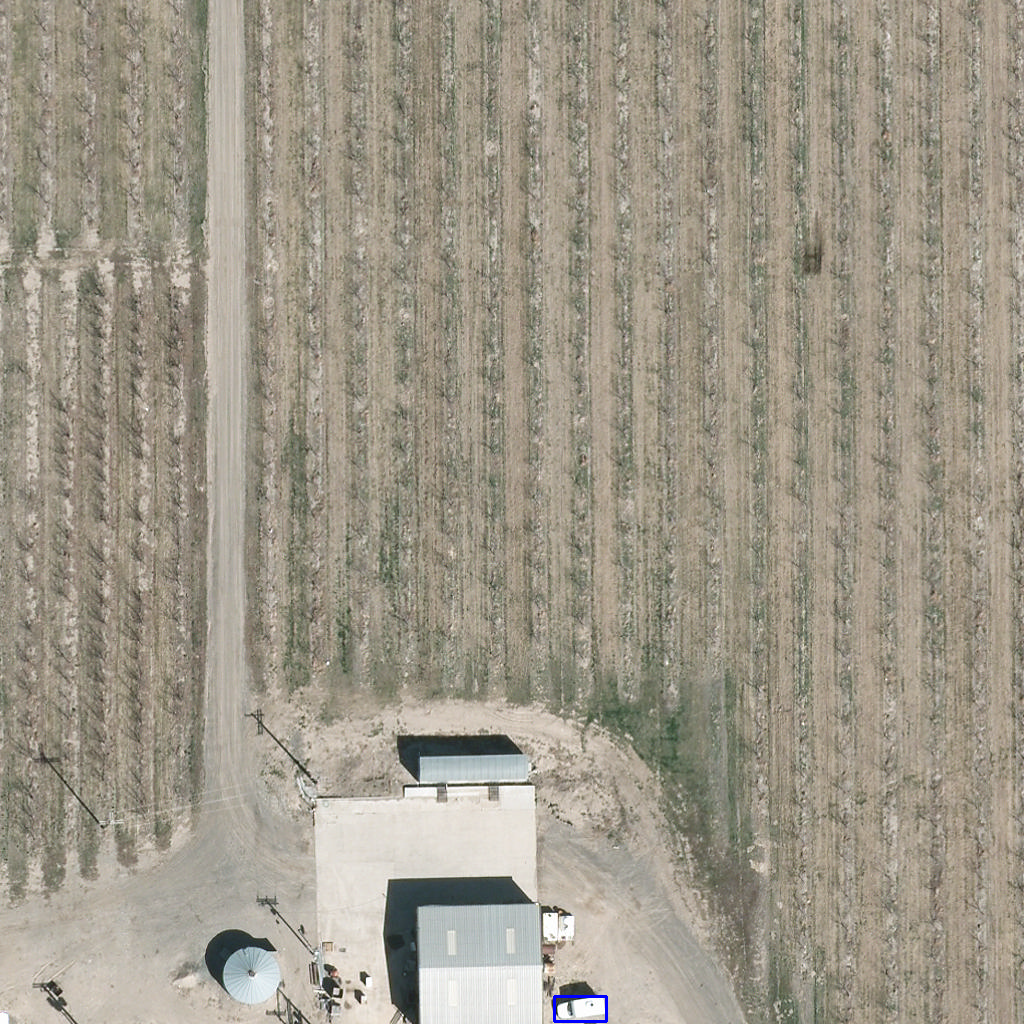
\includegraphics[trim={550pt 0pt 410pt 990pt},clip,width=\textwidth]{images/015Results/01abb_vs_obb/abb_truck.png}
        \caption{Label: "Truck", ABB format, area: $\approx 1378 \text{px}$}
        \label{fig:abb_truck}
    \end{subfigure}
    \hfill
    \begin{subfigure}[b]{0.45\textwidth}
        \centering
        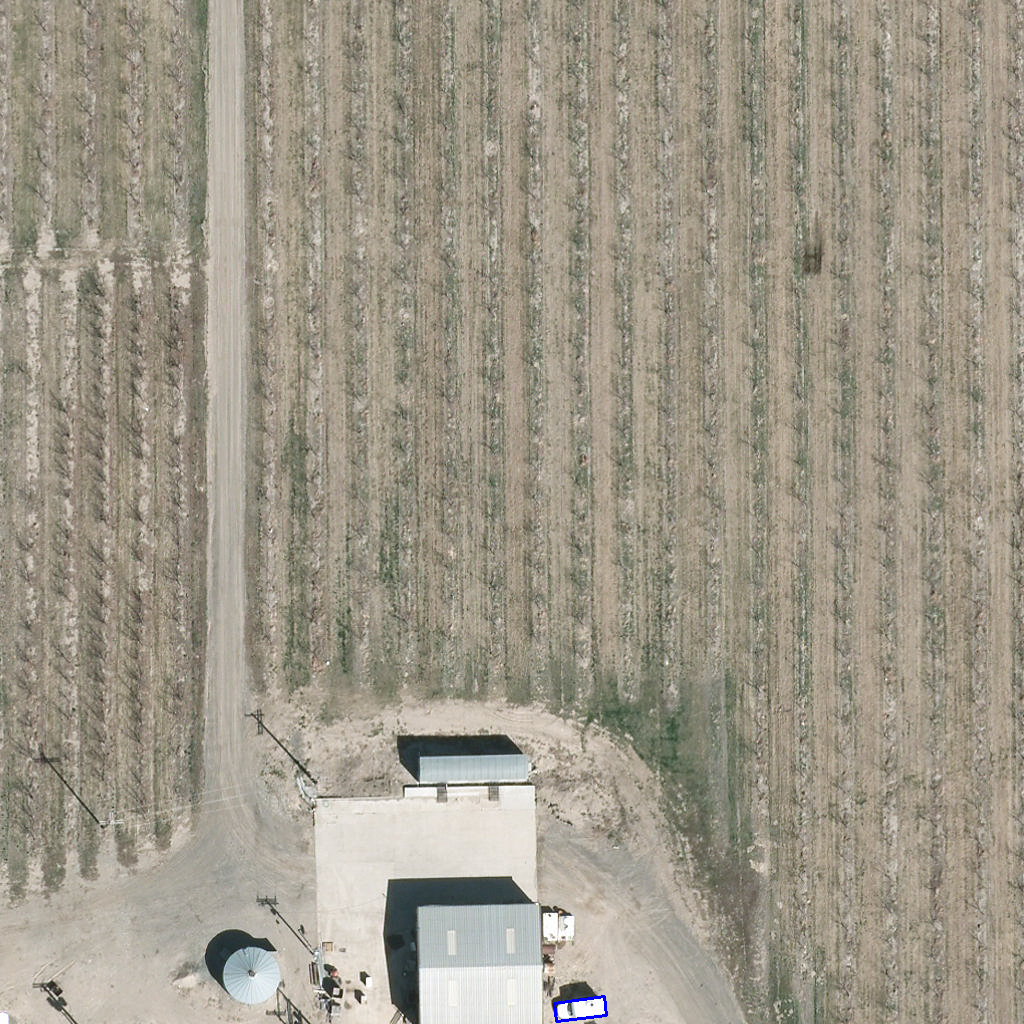
\includegraphics[trim={550pt 0pt 410pt 990pt},clip,width=\textwidth]{images/015Results/01abb_vs_obb/obb_truck.png}
        \caption{Label: "Truck", OBB format, area: $\approx 967 \text{px}$}
        \label{fig:obb_truck}
    \end{subfigure}
    
    \vspace{0.5cm} % Abstand zwischen den Zeilen
    
    % Zweite Zeile
    \begin{subfigure}[b]{0.45\textwidth}
        \centering
        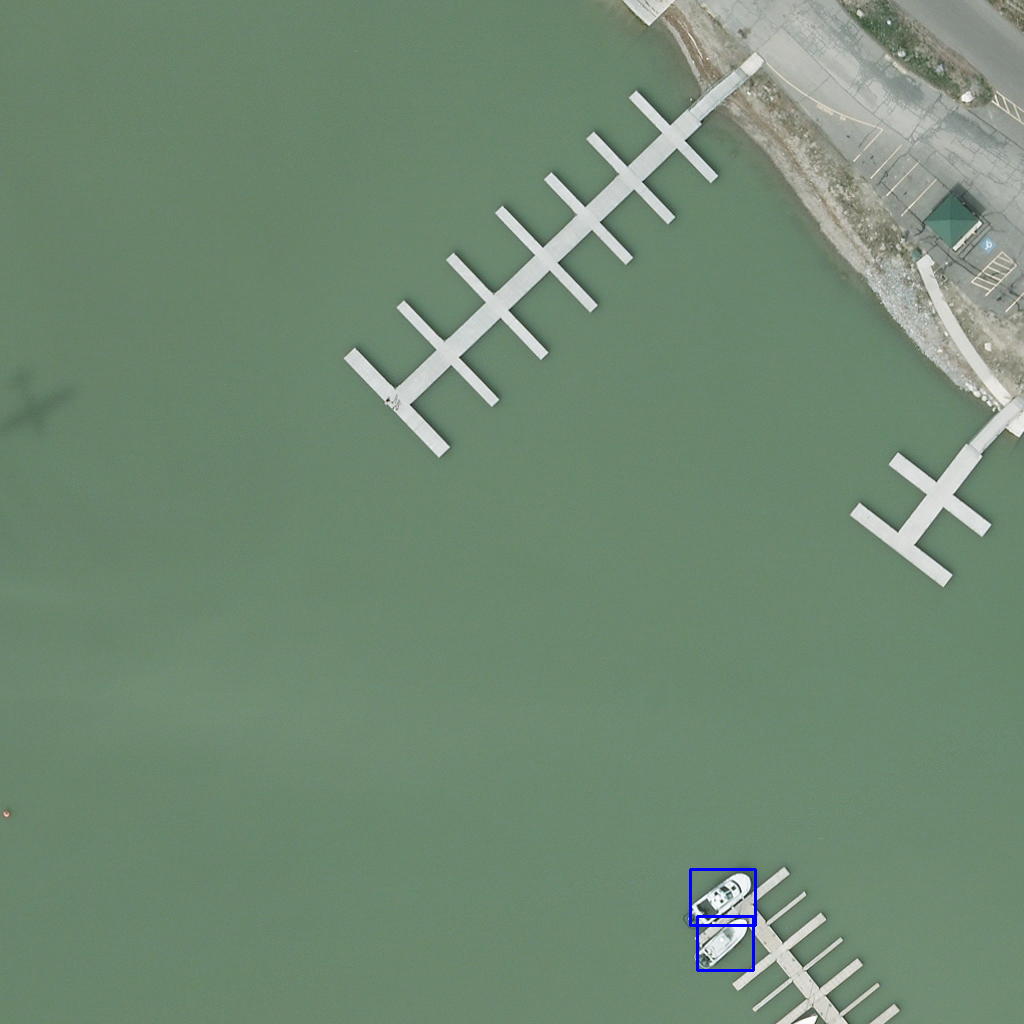
\includegraphics[trim={680pt 50pt 250pt 865pt},clip,width=\textwidth]{images/015Results/01abb_vs_obb/abb_ship.png}
        \caption{Labels: "Ship", ABB format}
        \label{fig:abb_ship}
    \end{subfigure}
    \hfill
    \begin{subfigure}[b]{0.45\textwidth}
        \centering
        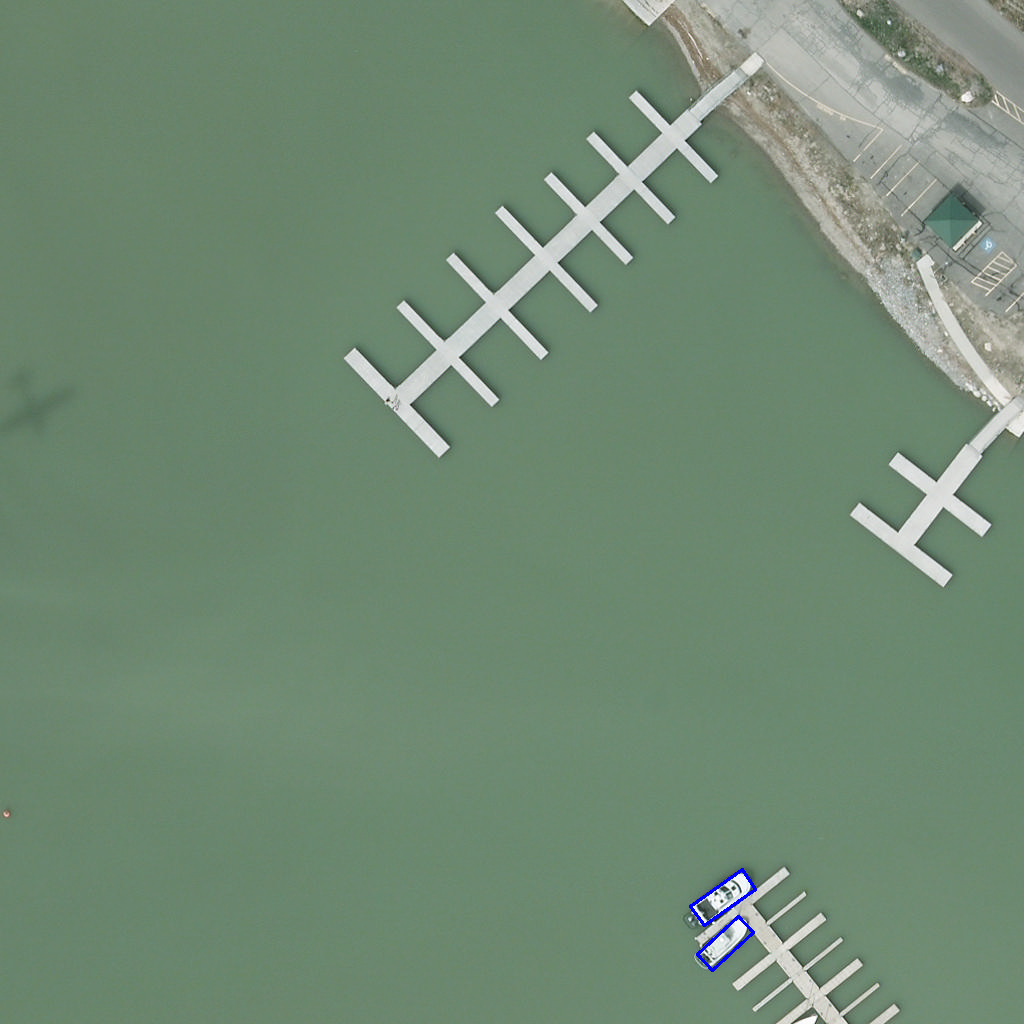
\includegraphics[trim={680pt 50pt 250pt 865pt},clip,width=\textwidth]{images/015Results/01abb_vs_obb/obb_ship.png}
        \caption{Labels: "Ship", OBB format}
        \label{fig:obb_ship}
    \end{subfigure}  
    \caption[Comparison of the bounding box formats of two different object classes]{Comparison of the bounding box formats of two different object classes (for full-sized images see \ref{fig:comparison_bb_format_fs}). \acrshort{obb} enclose objects much more accurately than \acrshort{abb}, as they include fewer irrelevant background areas. The reduced risk of overlap with neighbouring structures allows the model to extract more relevant object features and thus learn a more accurate representation of the classes (Own representation).
}
    \label{fig:comparison_bb_format}
\end{figure}
\todo{nicht nur erläutern was man sieht sondern auch was man daraus folgert (analyse) im Bildunterschrift}


Figure \ref{fig:comparison_bb_format} shows a comparison between \acrshort{obb} and \acrshort{abb} for different object classes. This difference is particularly clear in the truck example: in Figure \ref{fig:abb_truck}, \acrshort{abb} occupies a significantly larger area with approx. 1378 px than \acrshort{obb} in Figure \ref{fig:obb_truck} with approx. 967 px. When comparing highly rotated objects, such as the ships in Figure \ref{fig:abb_ship} and \ref{fig:obb_ship}, it can be seen that \acrshort{obb} encloses the object itself much more precisely and includes less of the surrounding area. Another advantage of \acrshort{obb} is the absence of overlaps between the boxes. For further examples, see Fig. \ref{fig:aab_obb_example_pics}. The line ‘ABB in OBB’ describes that the \acrshort{obb} model (\acrshort{YOLO}v9u) was trained with \acrshort{abb} bounding boxes. This means that the \acrshortpl{obb} in the \acrshort{VEDAI} dataset are converted to the bounding box format intended for \acrshort{YOLO}v9 (see \hyperlink{eq:yolov9u} {Equ.} in section \ref{sec:yolov9}) as \acrshort{abb} (i.e. with 8 coordinates that span an axis-parallel bounding box).
 

A comparison of all bounding box areas (see Figure \ref{fig:bbox_area}) shows that \acrshort{obb} is more compact on average (median \acrshort{abb}: approx. 1000 px, median \acrshort{obb}: >700 px). The \acrshort{abb} areas correspond almost exactly to the ‘ABB in OBB’ because the bounding boxes are almost identical; the only difference lies in the trained model and the calculations of the corners of the \acrshort{abb}. The bounding boxes occupy approximately 0.066\% of the total image area as \acrshort{obb} (approx. 700 px per box) and approximately 0.095\% as \acrshort{abb} (approx. 1000 px per box). This means that \acrshort{obb} is just below the lower limit for very small objects according to \citeauthor {Chen2017} \cite{Chen2017} (see section \ref{ch:state_of_research}) and are considered ‘very small objects’, while \acrshort{abb} is above the lower limit for small objects and is therefore considered a ‘small object’ (see \ref{ap:calc_bb_area_percent} for calculation).




\begin{figure}[htbp]
    \centering
    \includesvg[width=0.8\textwidth]{images/015Results/01abb_vs_obb/boxplot_areas.svg}
    \caption[Comparison of Bounding Box Area in pixels for \acrshort{abb}, \acrshort{obb}, abb in obb]{Comparison of Bounding Box Area in pixels for \acrshort{abb}, \acrshort{obb}, ABB in OBB. "ABB in OBB" means, that \acrlong{abb} converted to obb was used in the \acrshort{YOLO}v9u model with zero rotation. Due to their rotation-based adjustment, \acrshortpl{obb} are more compact than \acrshortpl{abb} and comprise less background. Since the calculation of ‘ABB in OBB’ areas yields almost identical values, it can be assumed that \acrshort{obb} models achieve higher performance due to more precise limitations (Own representation).}
    \label{fig:bbox_area}
\end{figure}


\begin{figure}[htbp]
    \centering
    \includesvg[width=0.8\textwidth]{images/015Results/01abb_vs_obb/abb_obb_best_val_on_val.svg}
    \caption[Comparison of \acrshort{mAP}@0.5--0.95 values for \acrshort{abb} and \acrshort{obb} (Best validation model on validation dataset)]{Comparison of \acrshort{mAP}@0.5--0.95 values for \acrshort{abb} and \acrshort{obb} (Best validation model on validation dataset). "ABB in OBB" means, that \acrlongpl{abb} converted to \acrshortpl{obb} was used in the \acrshort{YOLO}v9u model with zero rotation. \acrshort{abb} show a lower \acrshort{mAP}, presumably due to the model, while \acrshort{obb} are superior due to their better object adaptation. Notably, ‘ABB in OBB’ achieves higher values, which may indicate the strong rotation sensitivity of \acrshort{obb} (Own representation).}
    \label{fig:obb_abb_map50-95:val_on_val}
\end{figure}
The analysis of \acrshort{mAP}@0.5--0.95 of the best validation model on the validation dataset (Figure \ref{fig:obb_abb_map50-95:val_on_val}) shows that the \acrshort{obb} model performs better than the \acrshort{abb} model in all cases. All models used to evaluate the performance of \acrshort{obb} and \acrshort{abb} were trained exclusively on the basis of \acrshort{RGB} images. Interestingly, \acrshortpl{abb} achieves higher performance on the \acrshort{obb} model than the adapted \acrshort{obb} boxes within the same model (\acrshort{YOLO}v9u). The same phenomenon can also be observed on the test dataset (Figure \ref{fig:obb_abb_map50-95:val_on_test}), so that \acrshort{abb} in conjunction with the \acrshort{obb} model delivers better results. It is striking that for the \acrshort{abb}-based models (both \acrshort{abb} and ‘ABB in OBB’), fold 1 always achieved the best value on the validation dataset, while for the \acrshort{obb} model, fold 0 delivered the best results there (see Table \ref{tab:best_folds_area} and Fig. \ref{fig:obb_abb_map50-95:val_on_val}). The results of the respective folds with the highest \acrshort{mAP}@0.5--0.95 value from Fig. \ref{fig:obb_abb_map50-95:val_on_val} are marked by the red dot in Figure \ref{fig:obb_abb_map50-95:val_on_test}. According to Table \ref{tab:best_folds_area} and Fig. \ref{fig:obb_abb_map50-95:val_on_val}, fold 1 achieved the highest \acrshort{mAP} value in the \acrshort{abb} model. However, on the test fold, this fold 1 only achieved the lower quantile, as can be seen in Fig. \ref{fig:obb_abb_map50-95:val_on_test} at the red dot.


\begin{table}[h]
\centering
\begin{tabular}{l c c}
\hline
\textbf{Model} & \textbf{Best mAP Fold (Validation)} & \textbf{Best mAP Fold (Test)} \\ 
\hline
abb &  1 & 1 \\
obb &  0 & 0 \\
abb in obb &  1 & 1 \\
\hline
\end{tabular}
\caption{Best fold per model at Bounding Box format}
\label{tab:best_folds_area}
\end{table}


The effects of the different rotations of the detected objects can be seen in Figure \ref{fig:aab_obb_example_pics} using the class \texttt{plane} as an example. The bounding boxes differ significantly in terms of their rotation angles between the three models. Deviations in the overlap of the detected bounding boxes with the ground truth annotations, on the other hand, occur much less frequently, which explains the higher \acrshort{mAP} performance of the \acrshort{abb}-based models. Other notable features, such as the difficulties in separating objects from the background, are discussed in the following sections.

Due to the lower probability of overlap errors and the more precise object contouring, the \acrshort{obb} format was selected for performing the permutation tests.


\begin{figure}[htbp]
    \centering
    \includesvg[width=0.8\textwidth]{images/015Results/01abb_vs_obb/aab_obb_best_val_on_test.svg}
    \caption[Comparison of \acrshort{mAP}@0.5--0.95 values for \acrshort{abb} and \acrshort{obb} (Best validation model on test dataset)]{Comparison of \acrshort{mAP}@0.5--0.95 values for \acrshort{abb} and \acrshort{obb} (Best validation model on test dataset). "ABB in OBB" means, that \acrlongpl{abb} converted to \acrshortpl{obb} was used in the \acrshort{YOLO}v9u model with zero rotation. The red dot is the fold, that has the best \acrshort{mAP}50-95 at the validation dataset (see fig. \ref{fig:obb_abb_map50-95:val_on_val}).  On the test dataset, \acrshort{abb} achieves poorer results, presumably due to model limitations, while \acrshort{obb} achieves significantly better performance due to more precise object boundaries. The ‘ABB in OBB’ configuration shows the best performance, as even small rotation deviations in the \acrshort{obb} model strongly influence the \acrshort{mAP} and the model's \acrshort{GT} \acrshort{BB} are significantly larger (Own representation). }
    \label{fig:obb_abb_map50-95:val_on_test}
\end{figure}

%##########################################################################
%##########################################################################

\begin{figure}[h!]
\centering
\renewcommand{\arraystretch}{1.2} % mehr Platz zwischen Zeilen
\setlength{\tabcolsep}{2pt} % weniger Platz zwischen Spalten
\begin{tabularx}{\textwidth}{c|*{9}{X}}
    & \textbf{Car}
    & \textbf{Truck}
    & \textbf{Camping Car}
    & \textbf{Tractor}
    & \textbf{Plane}
    & \textbf{Ship}
    & \textbf{Vehicle}
    & \textbf{Pick-Up}
    & \textbf{Van} \\ \hline
    \rotatebox{90}{\textbf{\acrshort{GT} (\acrshort{abb})}} 
    %Car
    & 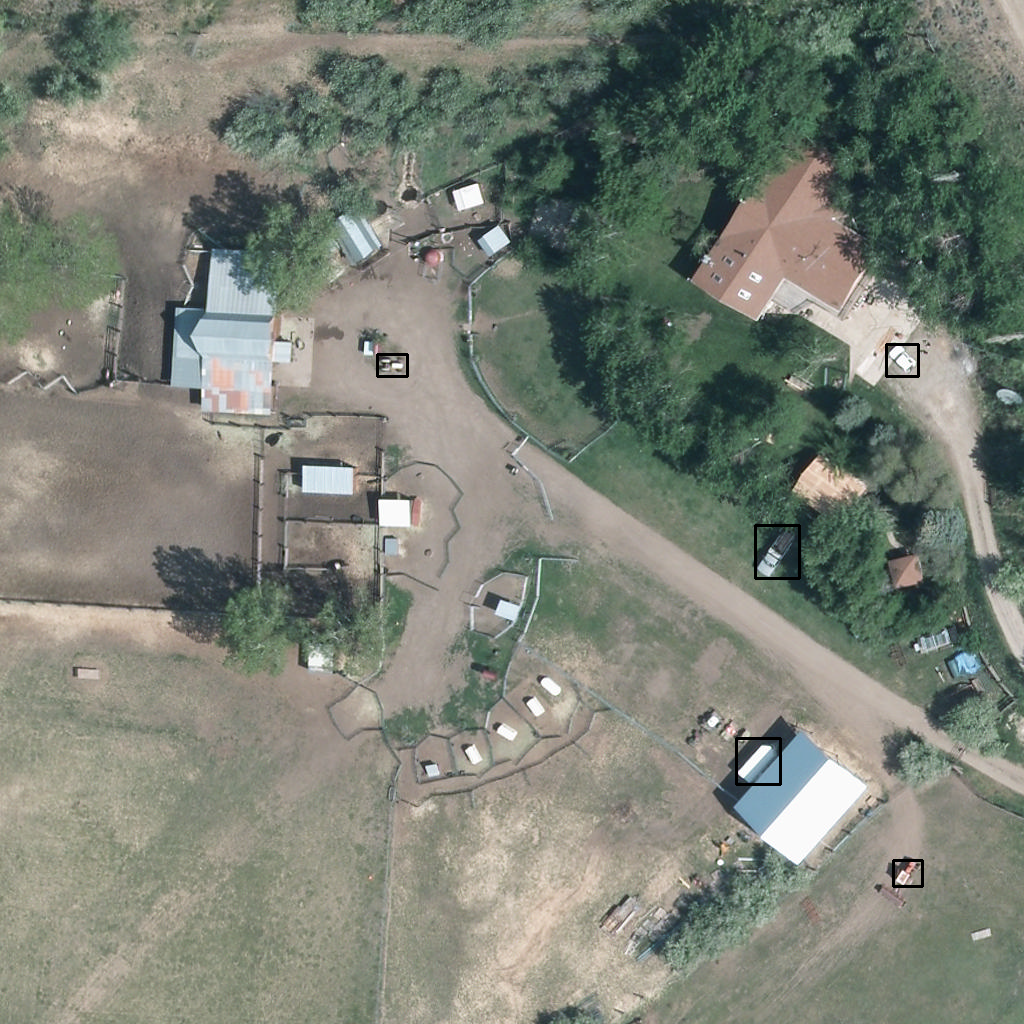
\includegraphics[trim={880pt 630pt 70pt 330pt},clip,width=\linewidth]{images/015Results/01abb_vs_obb/comp_images/ground_truth_abb/523.png}
    %Truck
    & 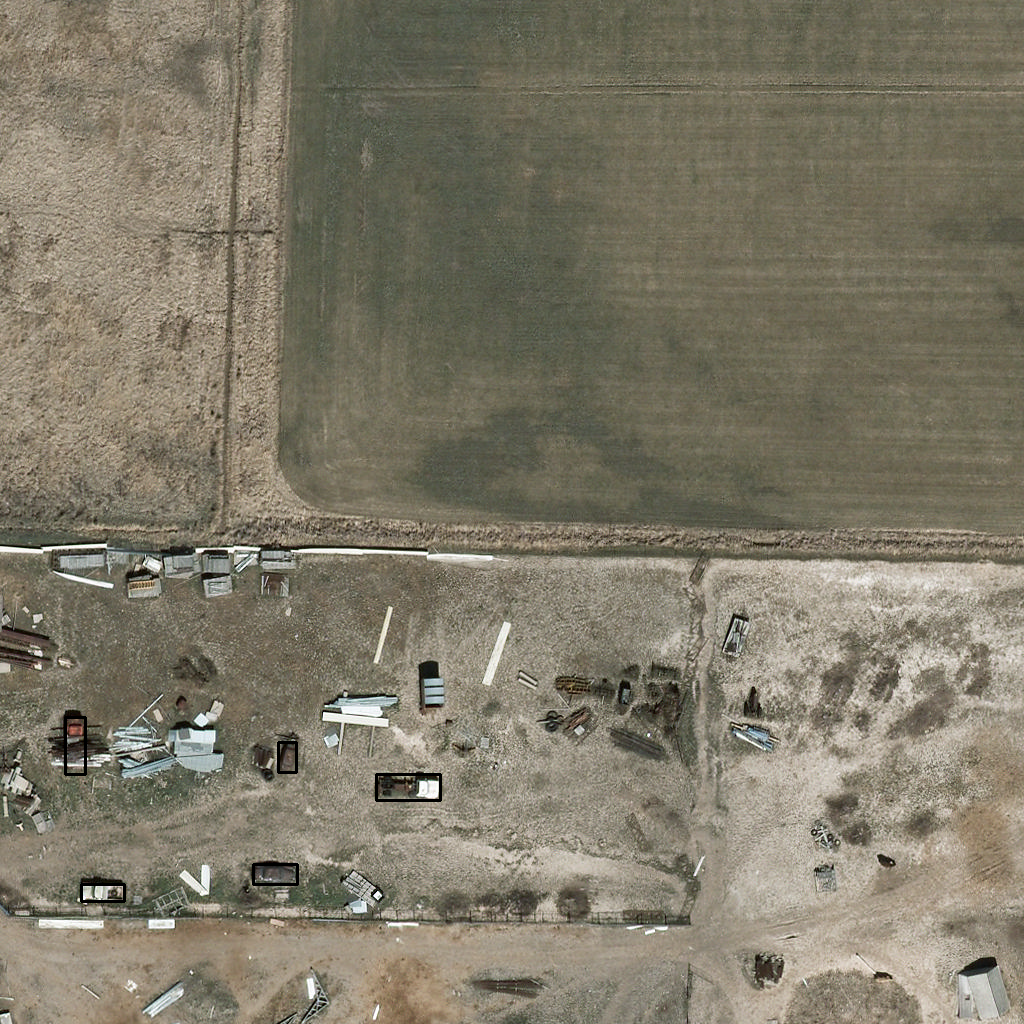
\includegraphics[trim={360pt 200pt 540pt 715pt},clip,width=\linewidth]{images/015Results/01abb_vs_obb/comp_images/ground_truth_abb/212.png}
    %Camping Car
    & 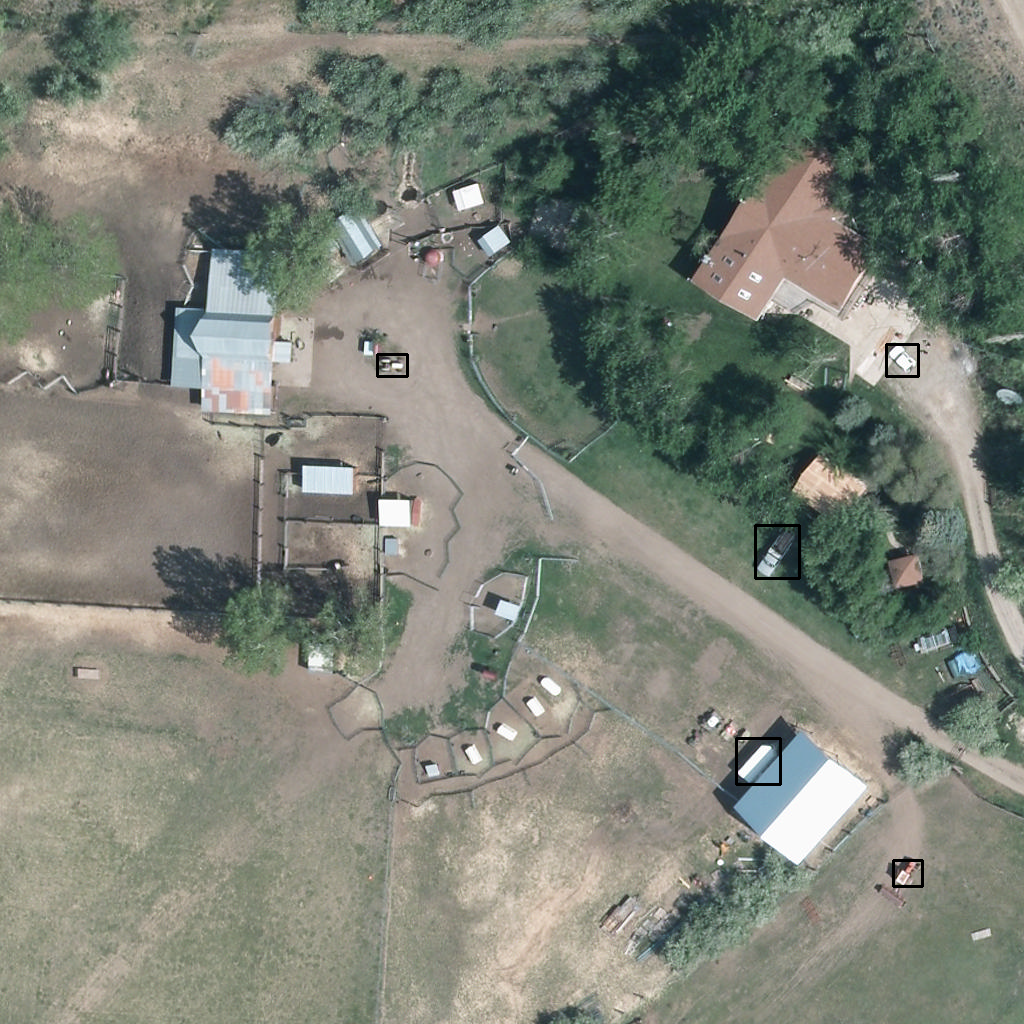
\includegraphics[trim={730pt 220pt 200pt 720pt},clip,width=\linewidth]{images/015Results/01abb_vs_obb/comp_images/ground_truth_abb/523.png}
    %Tractor
    & 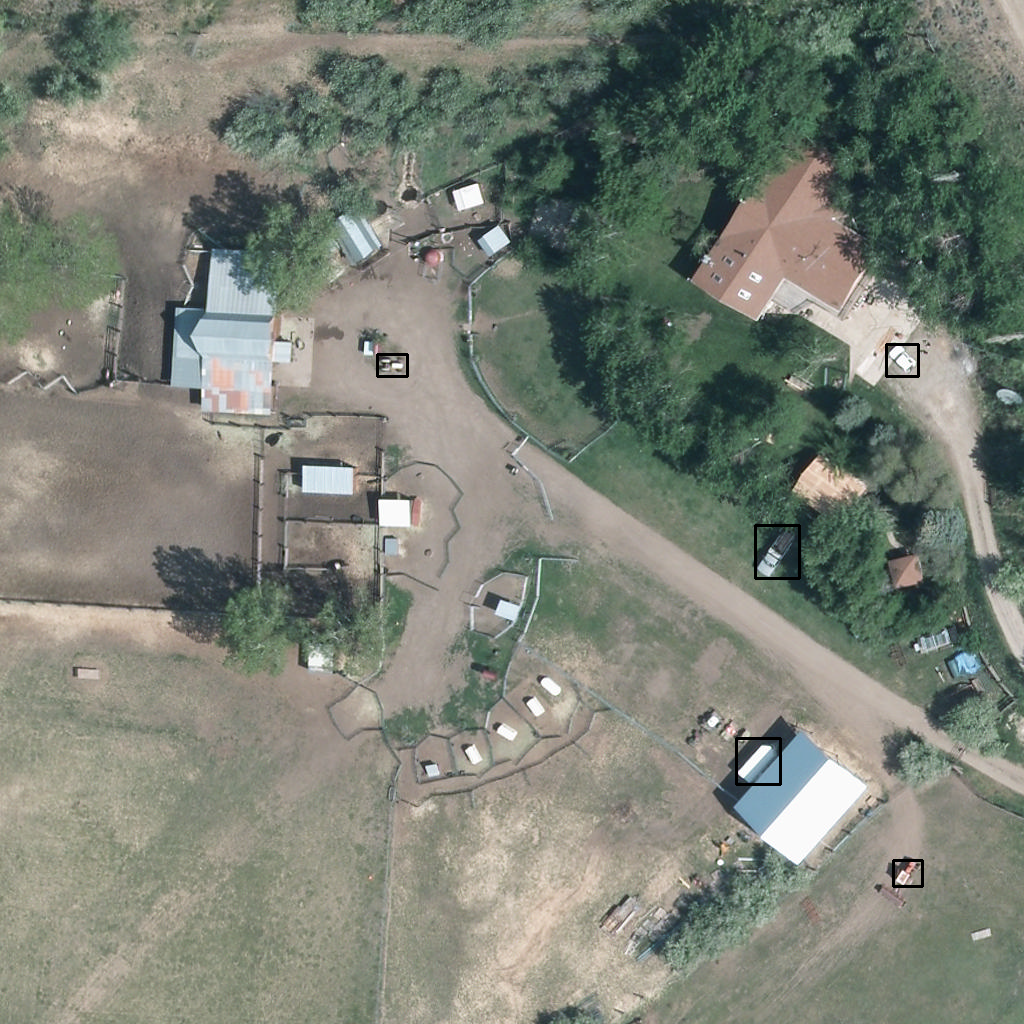
\includegraphics[trim={850pt 110pt 80pt 830pt},clip,width=\linewidth]{images/015Results/01abb_vs_obb/comp_images/ground_truth_abb/523.png}
    %Plane
    &  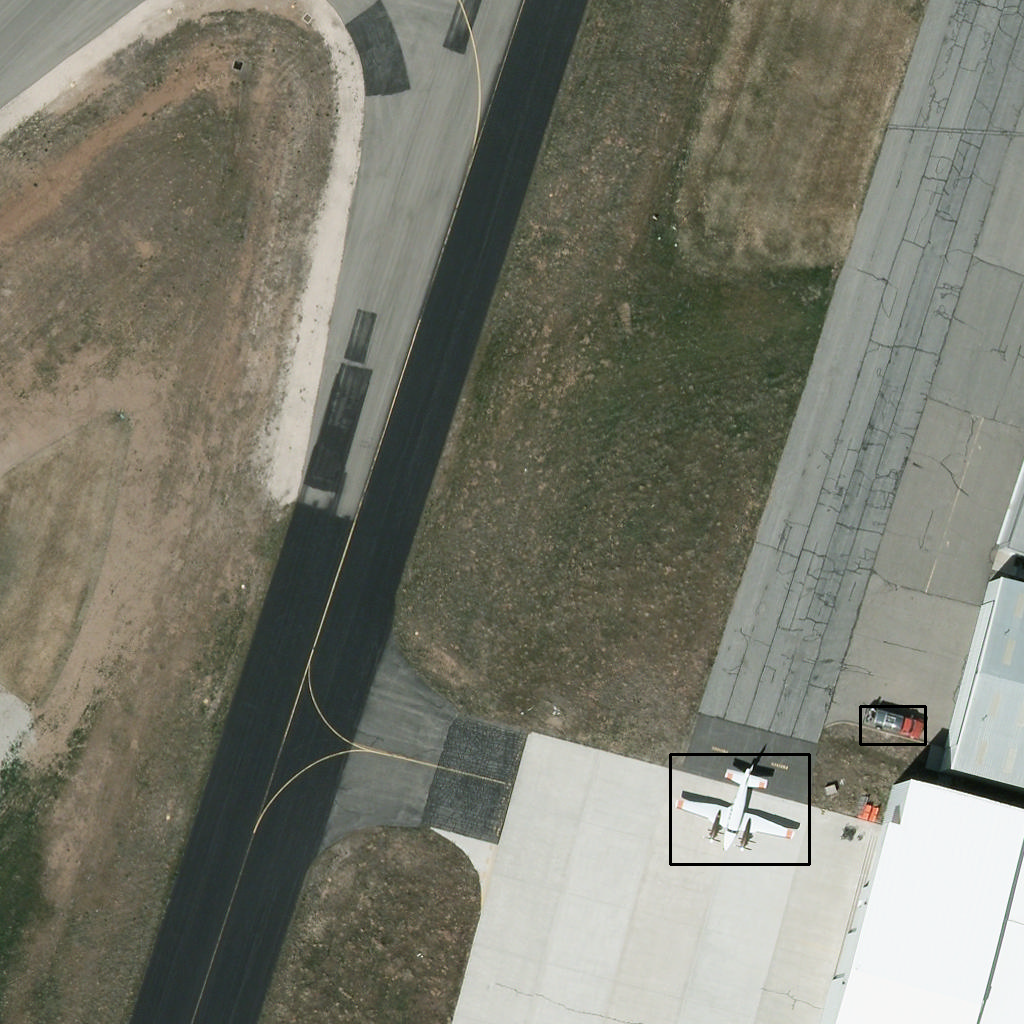
\includegraphics[trim={650pt 120pt 170pt 720pt},clip,width=\linewidth]{images/015Results/01abb_vs_obb/comp_images/ground_truth_abb/487.png}
    %Ship
    & 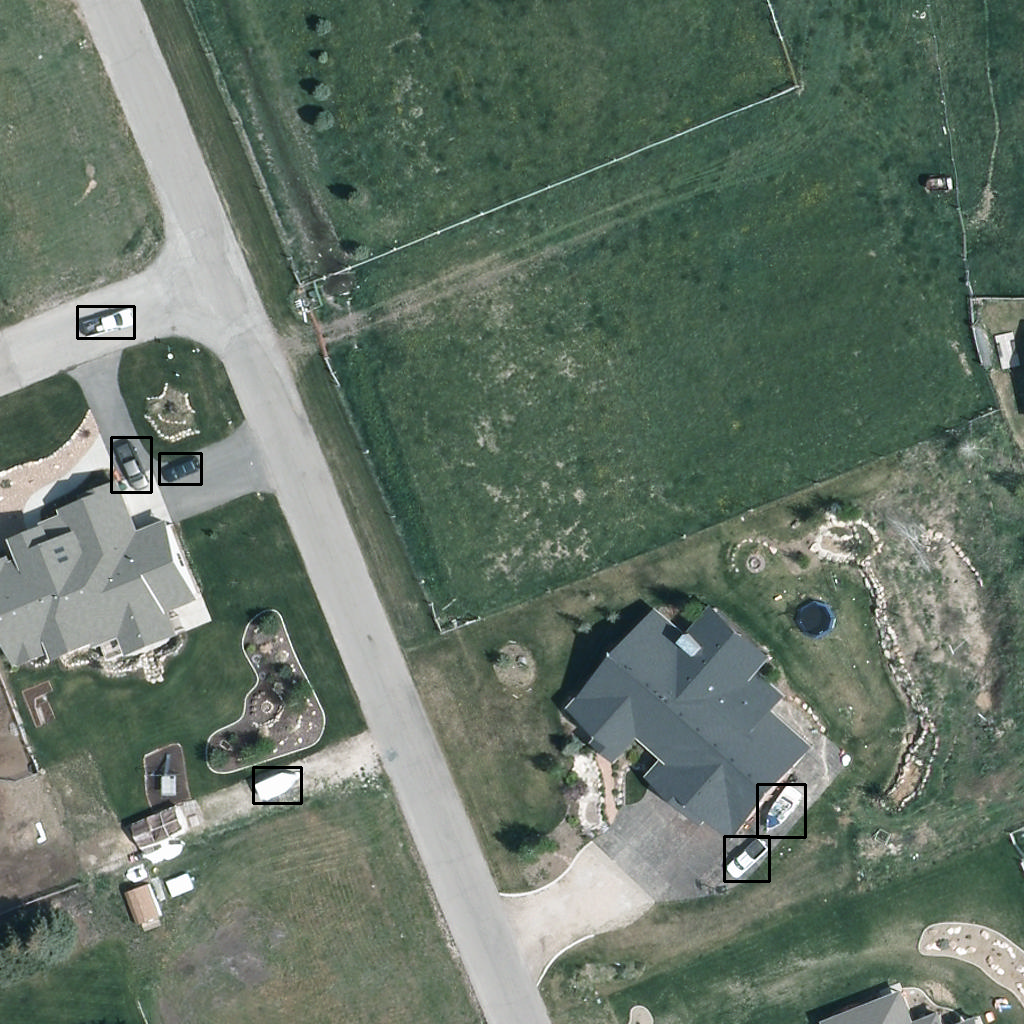
\includegraphics[trim={230pt 200pt 680pt 725pt},clip,width=\linewidth]{images/015Results/01abb_vs_obb/comp_images/ground_truth_abb/509.png}
    %vehicle
    & 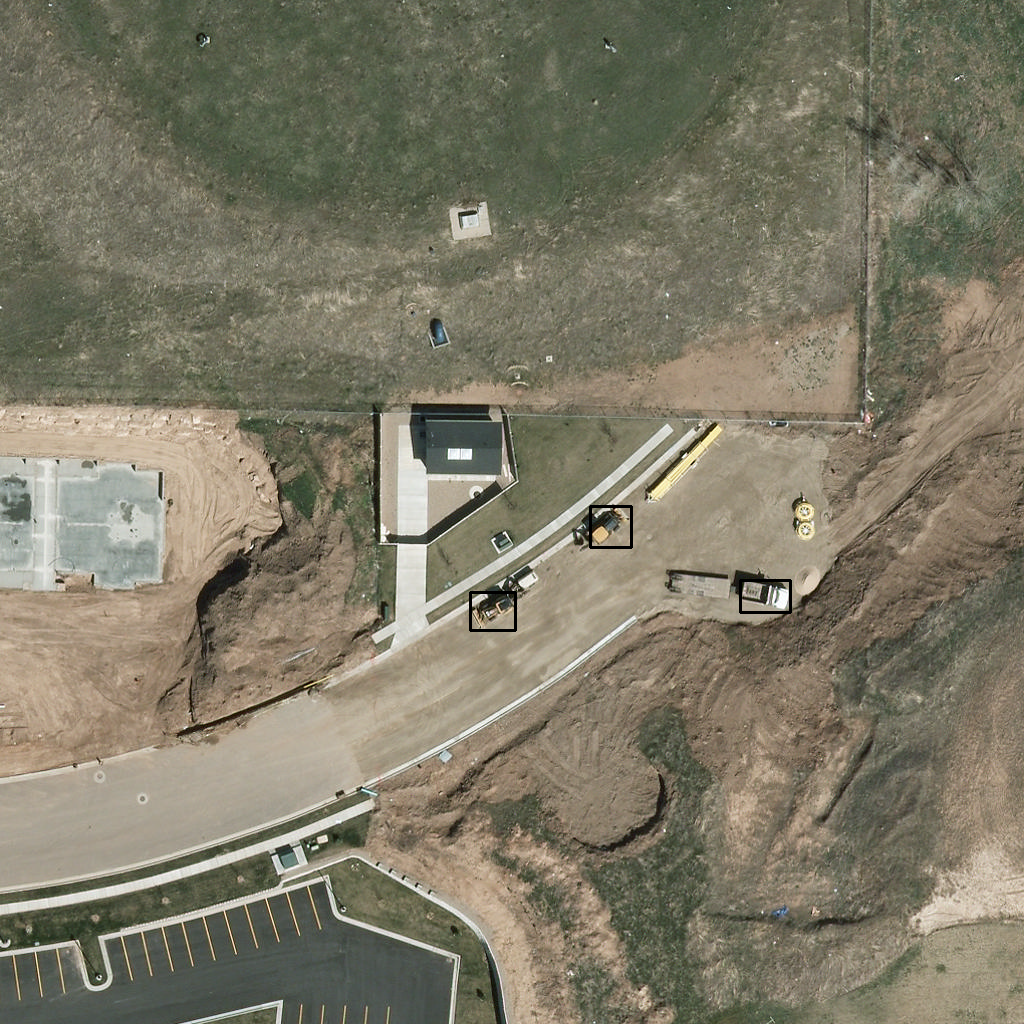
\includegraphics[trim={440pt 360pt 460pt 555pt},clip,width=\linewidth]{images/015Results/01abb_vs_obb/comp_images/ground_truth_abb/427.png}
    %Pick Up
    & 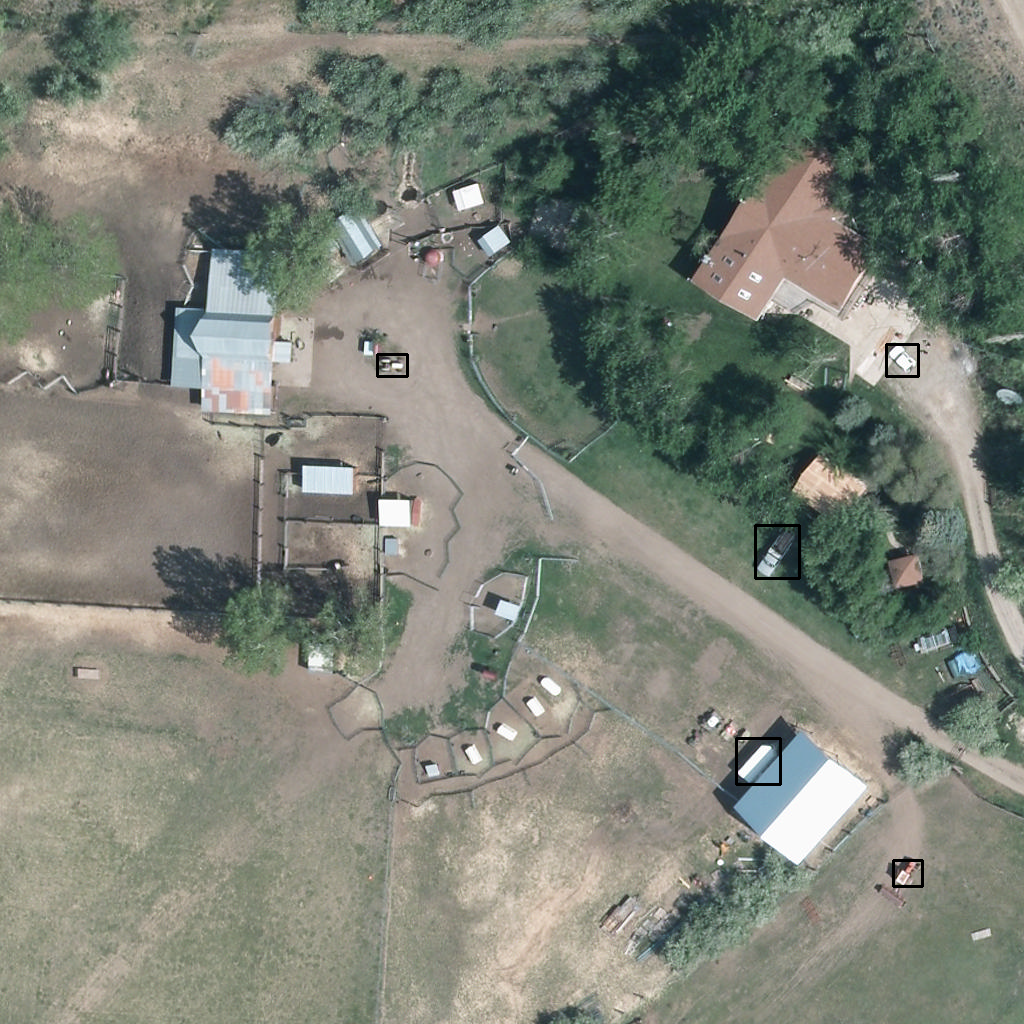
\includegraphics[trim={740pt 420pt 180pt 510pt},clip,width=\linewidth]{images/015Results/01abb_vs_obb/comp_images/ground_truth_abb/523.png}
    %Van
    & 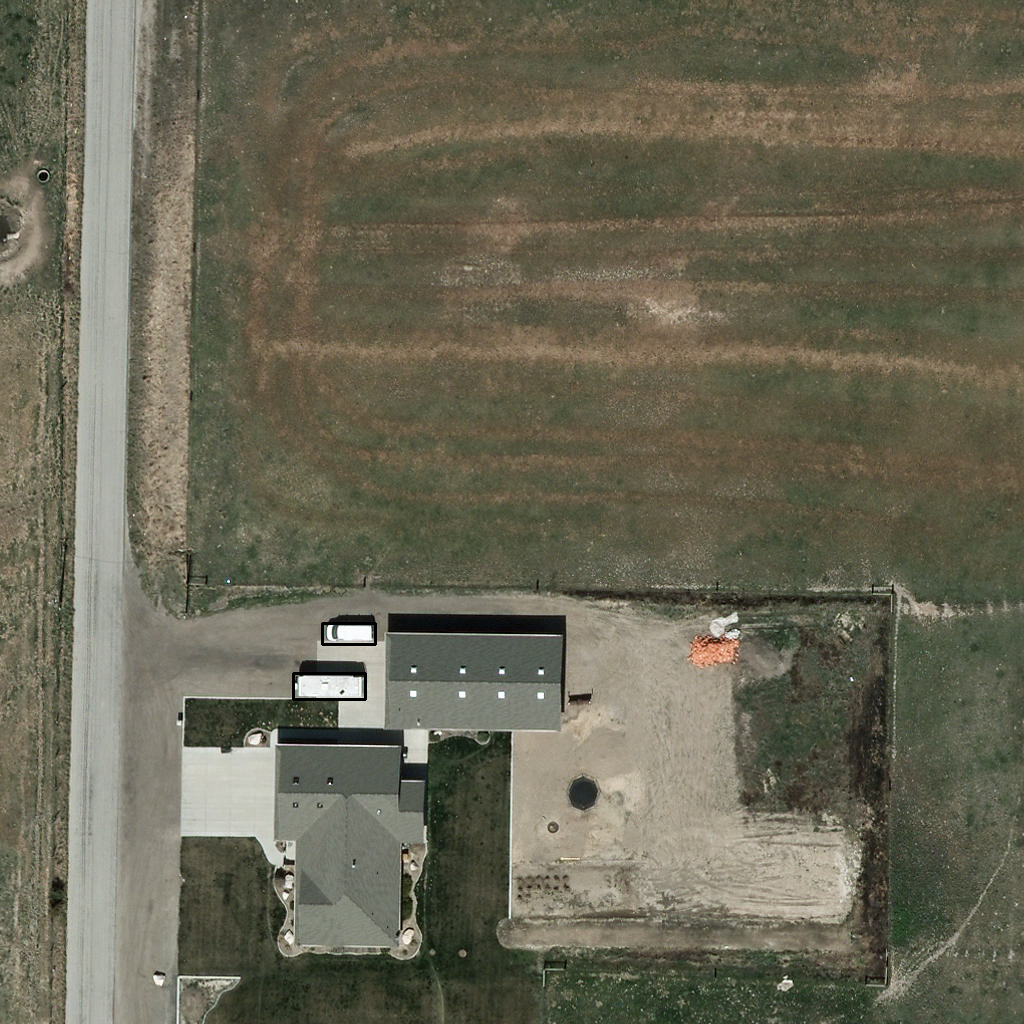
\includegraphics[trim={300pt 355pt 610pt 570pt},clip,width=\linewidth]{images/015Results/01abb_vs_obb/comp_images/ground_truth_abb/198.png} \\ \hline

    \rotatebox{90}{\textbf{\acrshort{GT} (\acrshort{obb})}} 
    %Car
    & 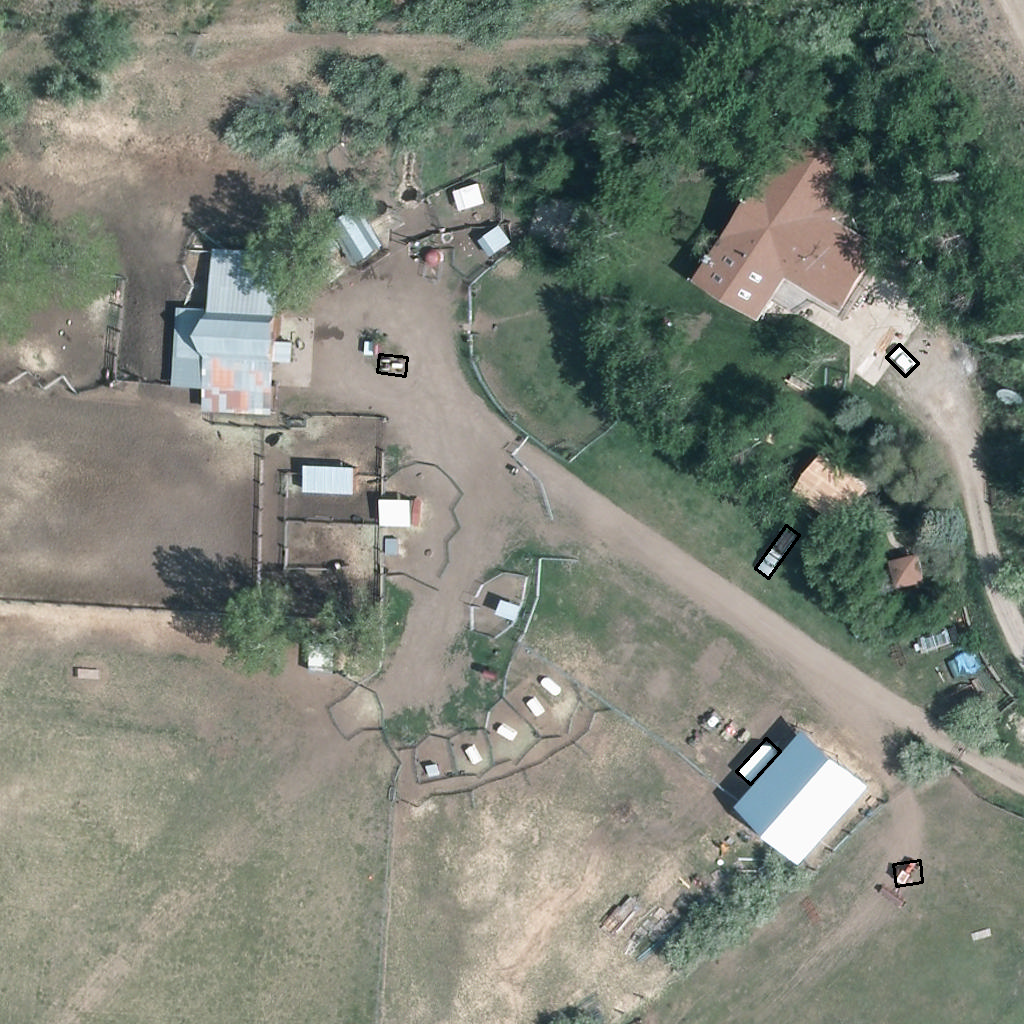
\includegraphics[trim={880pt 630pt 70pt 330pt},clip,width=\linewidth]{images/015Results/01abb_vs_obb/comp_images/ground_truth_obb/523.png}
    %Truck
    & 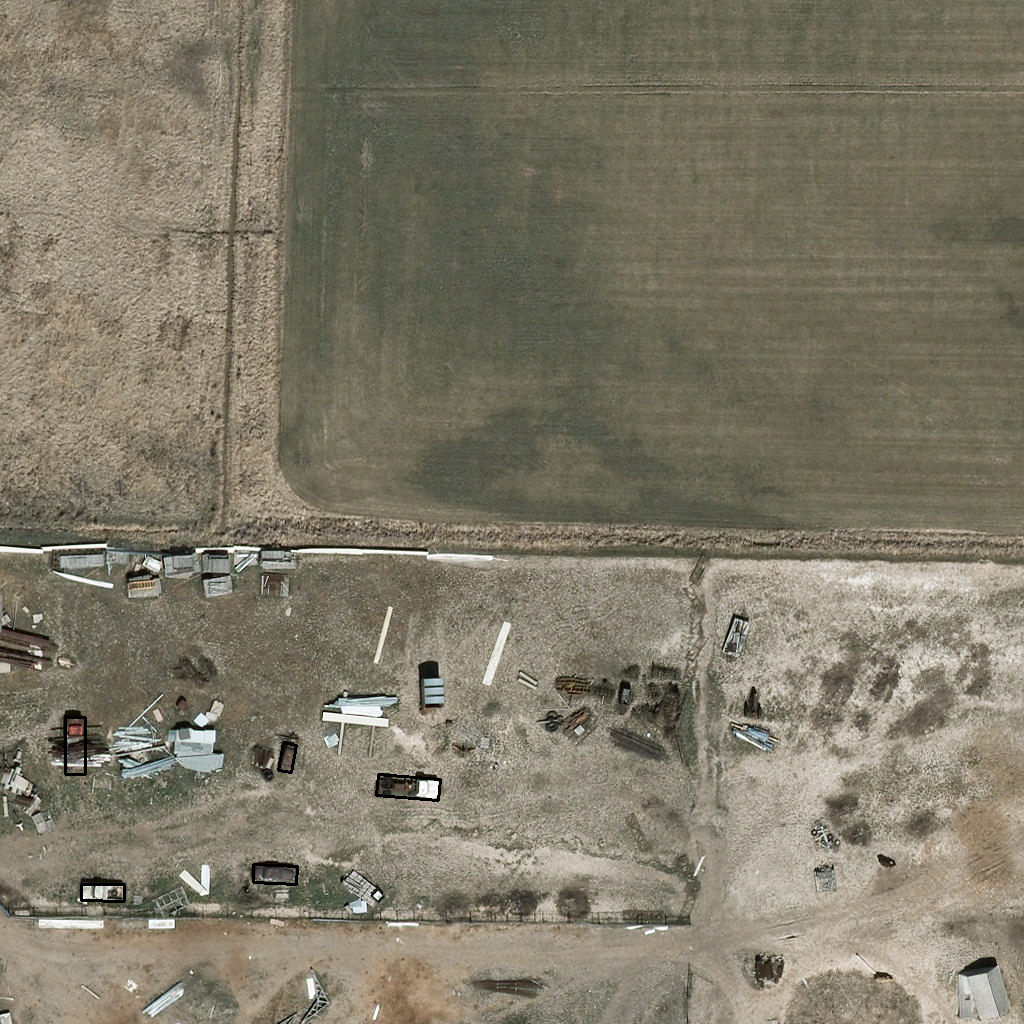
\includegraphics[trim={360pt 200pt 540pt 715pt},clip,width=\linewidth]{images/015Results/01abb_vs_obb/comp_images/ground_truth_obb/212.png}
    %Camping Car
    & 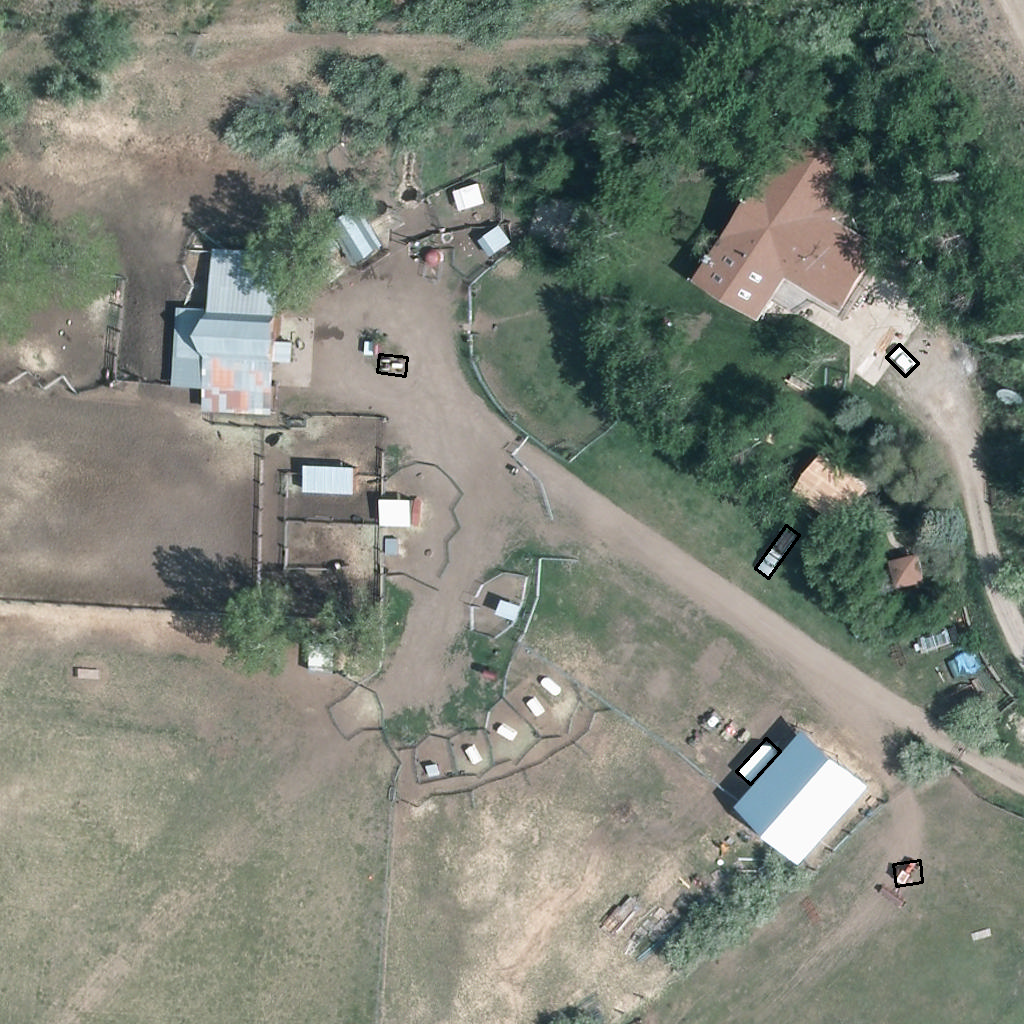
\includegraphics[trim={730pt 220pt 200pt 720pt},clip,width=\linewidth]{images/015Results/01abb_vs_obb/comp_images/ground_truth_obb/523.png}
    %Tractor
    & 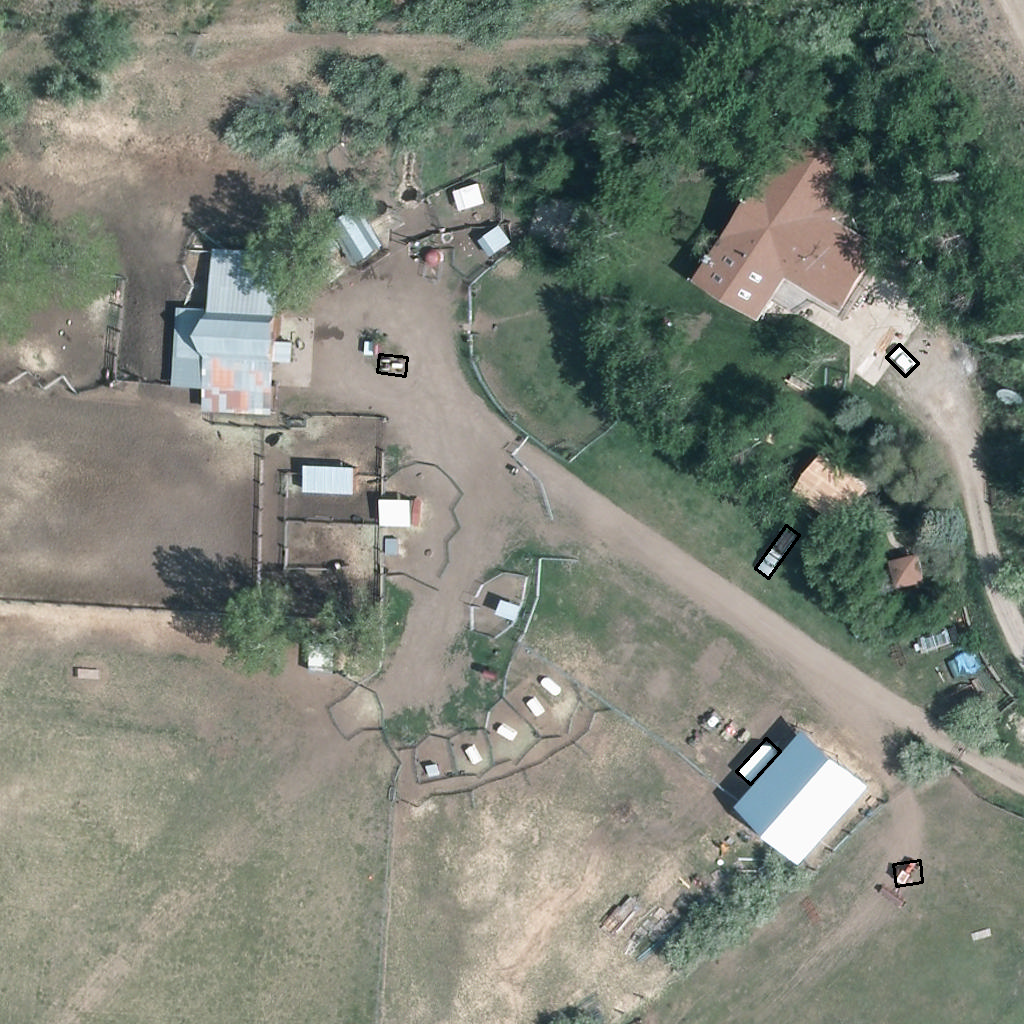
\includegraphics[trim={850pt 110pt 80pt 830pt},clip,width=\linewidth]{images/015Results/01abb_vs_obb/comp_images/ground_truth_obb/523.png}
    %Plane
    &  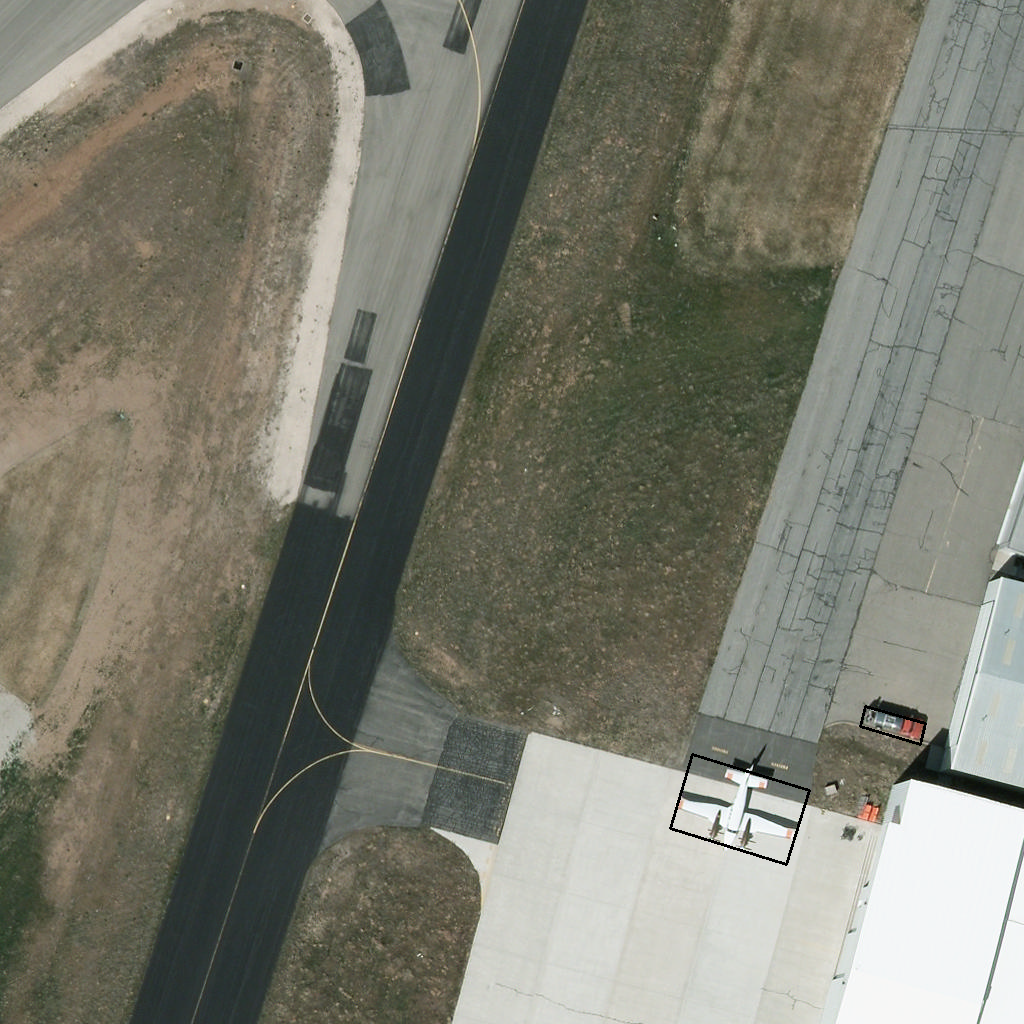
\includegraphics[trim={650pt 120pt 170pt 720pt},clip,width=\linewidth]{images/015Results/01abb_vs_obb/comp_images/ground_truth_obb/487.png}
    %Ship
    & 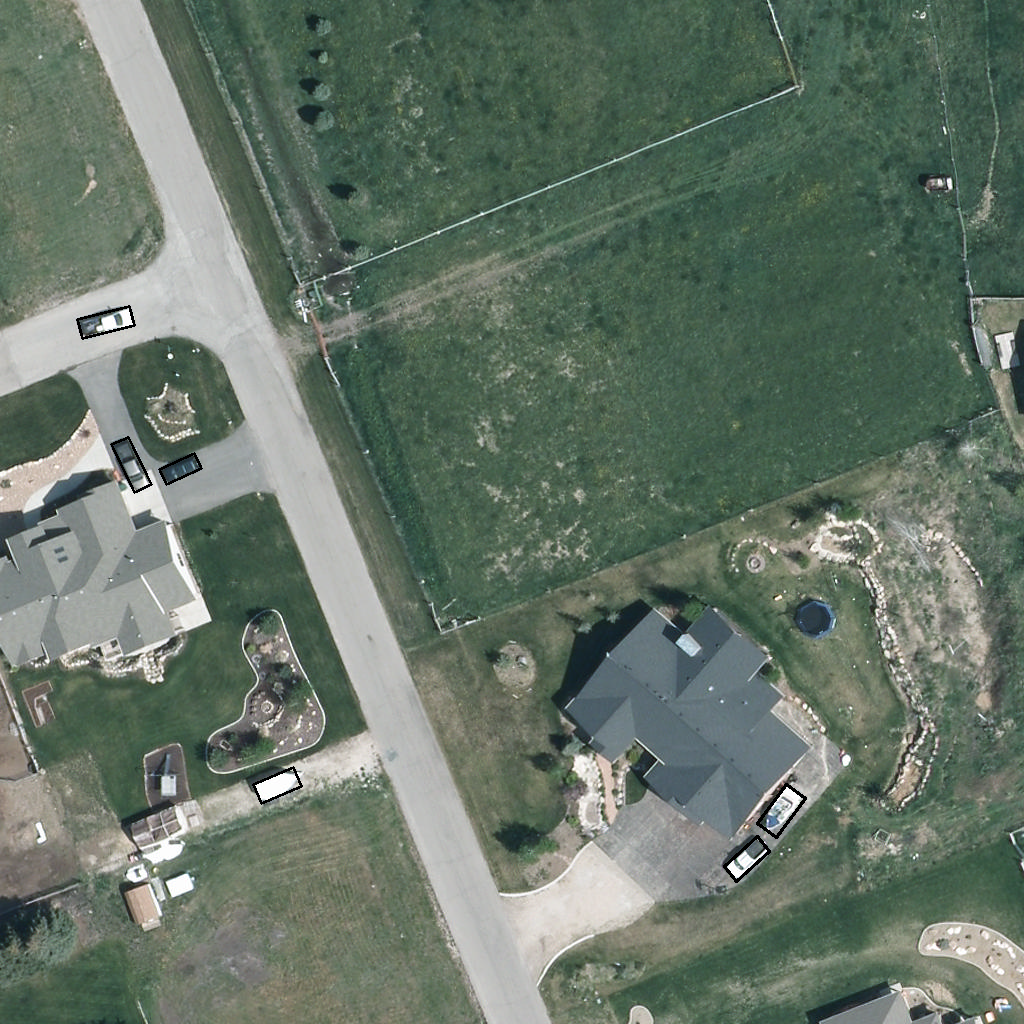
\includegraphics[trim={230pt 200pt 680pt 725pt},clip,width=\linewidth]{images/015Results/01abb_vs_obb/comp_images/ground_truth_obb/509.png}
    %vehicle
    & 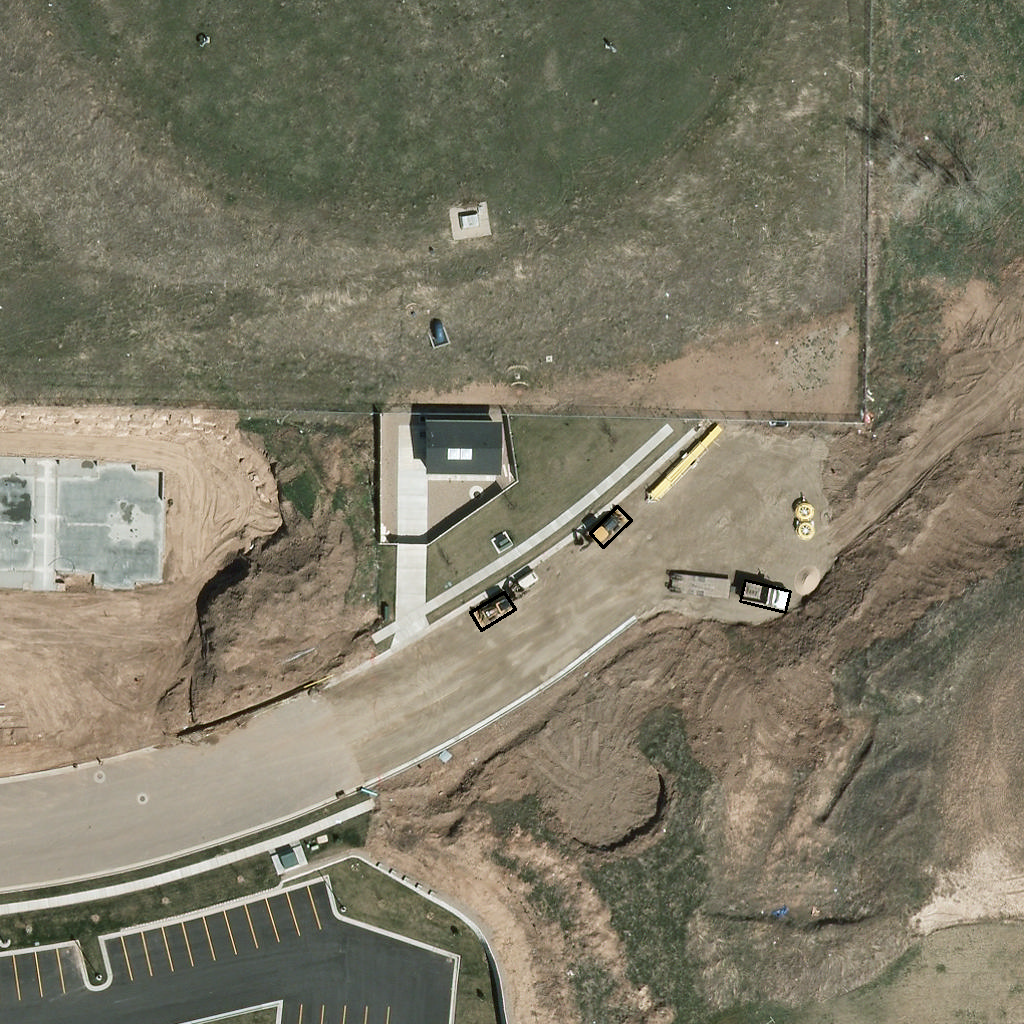
\includegraphics[trim={440pt 360pt 460pt 555pt},clip,width=\linewidth]{images/015Results/01abb_vs_obb/comp_images/ground_truth_obb/427.png}
    %Pick Up
    & 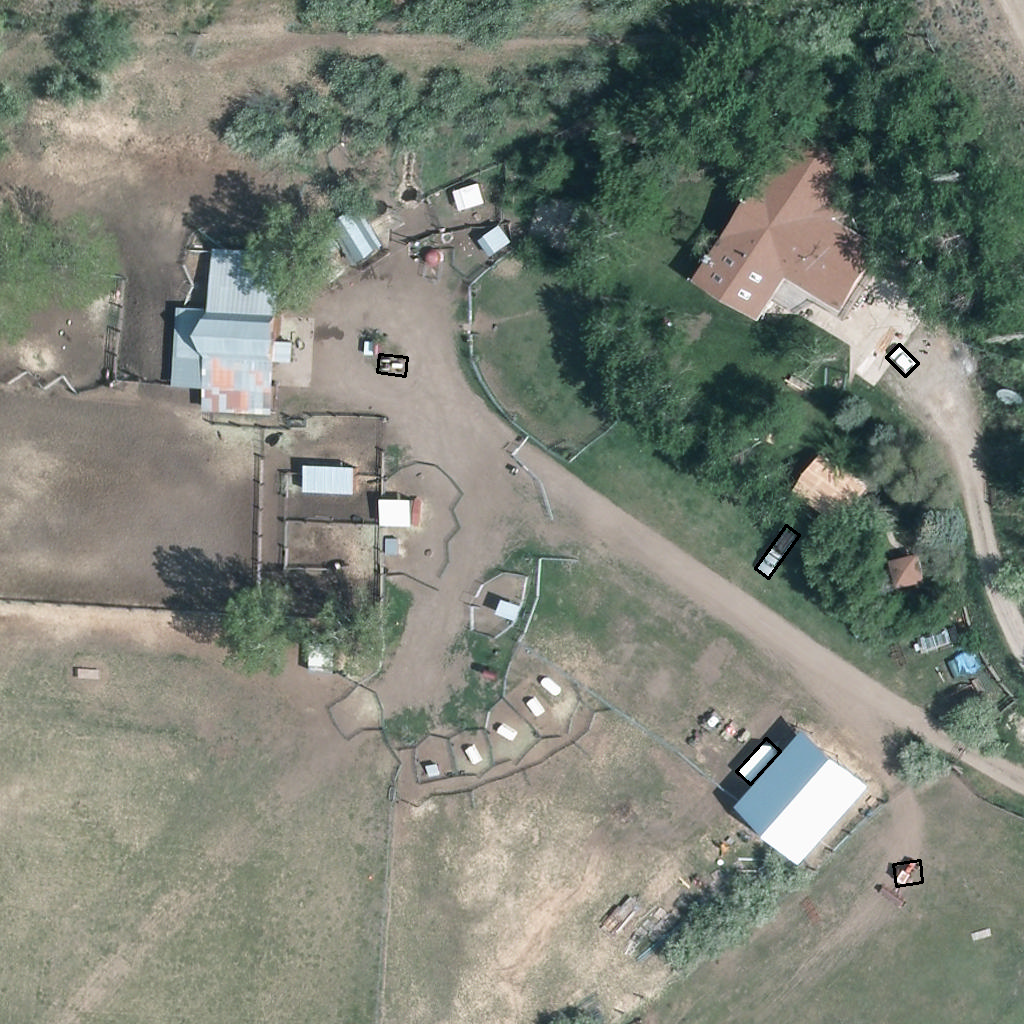
\includegraphics[trim={740pt 420pt 180pt 510pt},clip,width=\linewidth]{images/015Results/01abb_vs_obb/comp_images/ground_truth_obb/523.png}
    %Van
    & 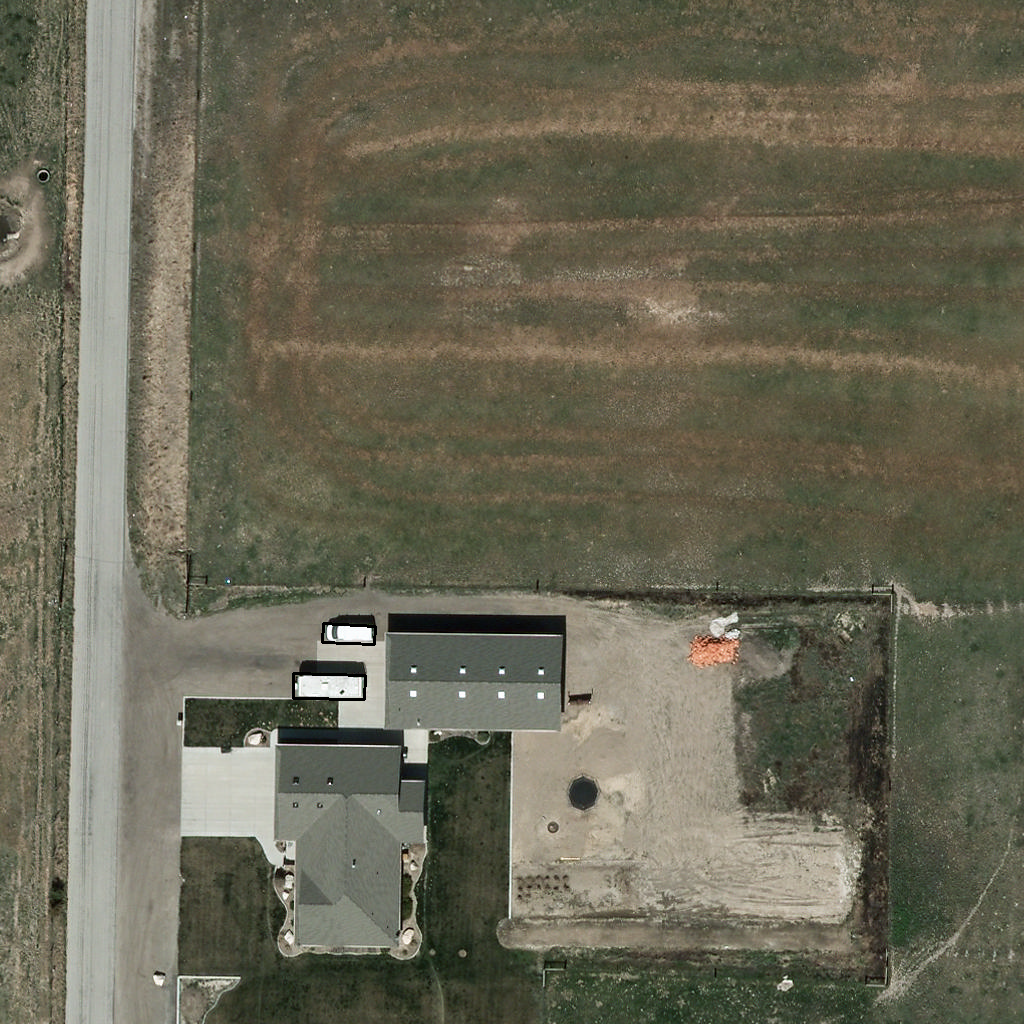
\includegraphics[trim={300pt 355pt 610pt 570pt},clip,width=\linewidth]{images/015Results/01abb_vs_obb/comp_images/ground_truth_obb/198.png} \\ \hline
    \rotatebox{90}{\textbf{\acrshort{abb}}} 
    %Car
    & 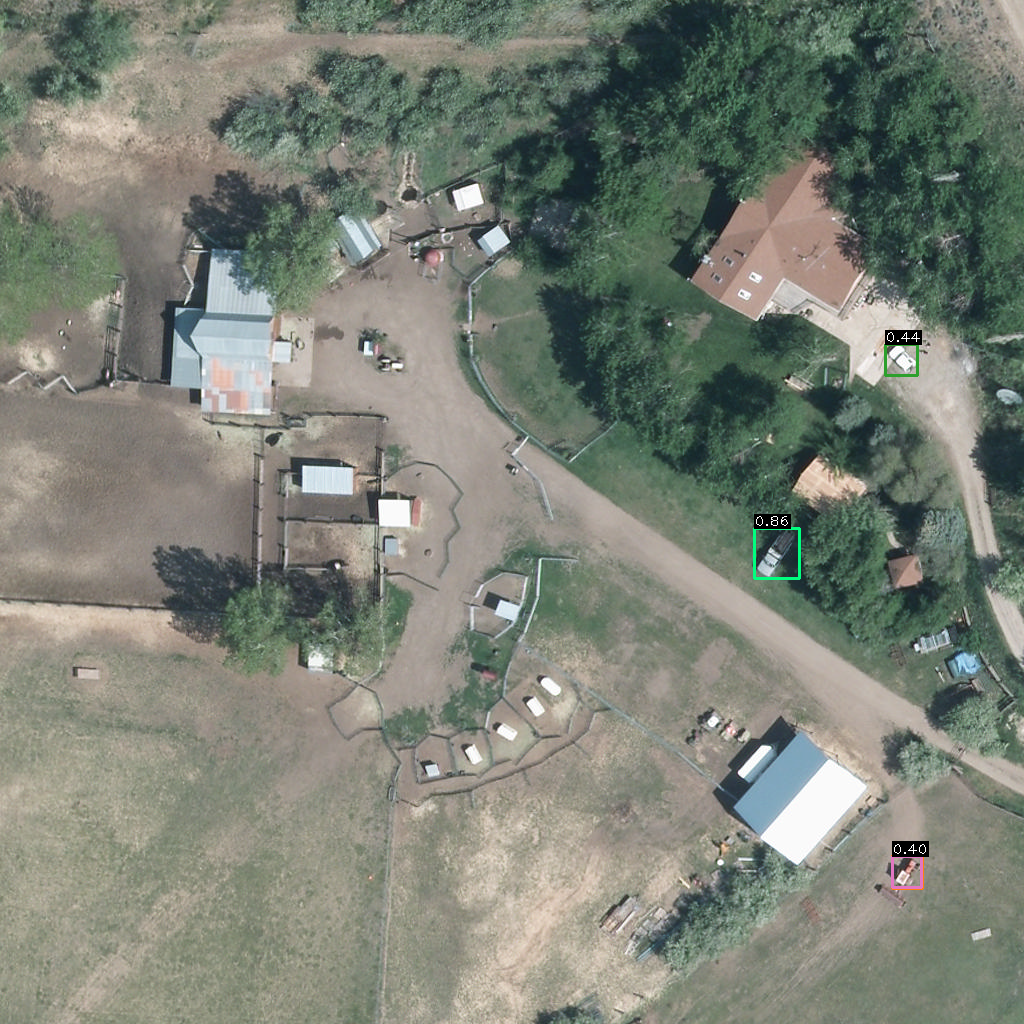
\includegraphics[trim={880pt 630pt 70pt 330pt},clip,width=\linewidth]{images/015Results/01abb_vs_obb/comp_images/abb/523.png}
    %Truck
    & 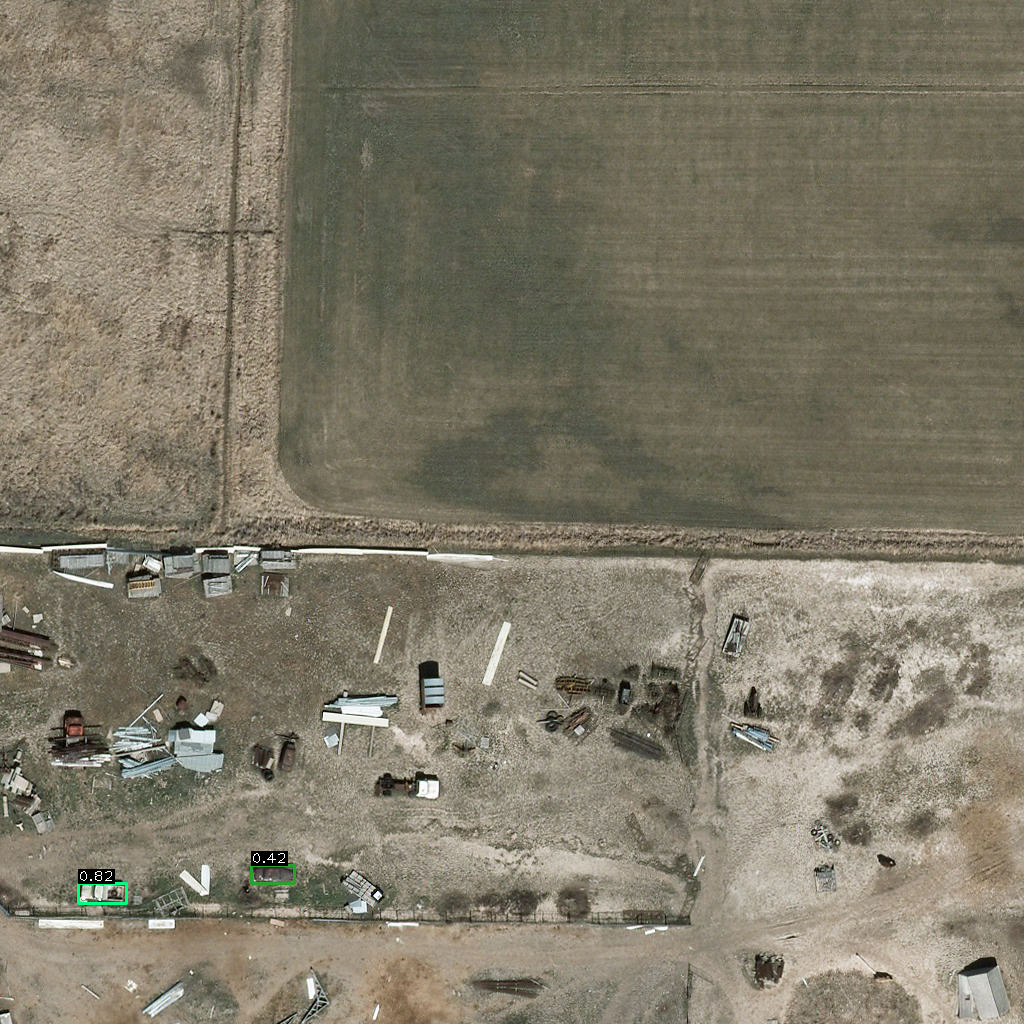
\includegraphics[trim={360pt 200pt 540pt 715pt},clip,width=\linewidth]{images/015Results/01abb_vs_obb/comp_images/abb/212.png}
    %Camping Car
    & 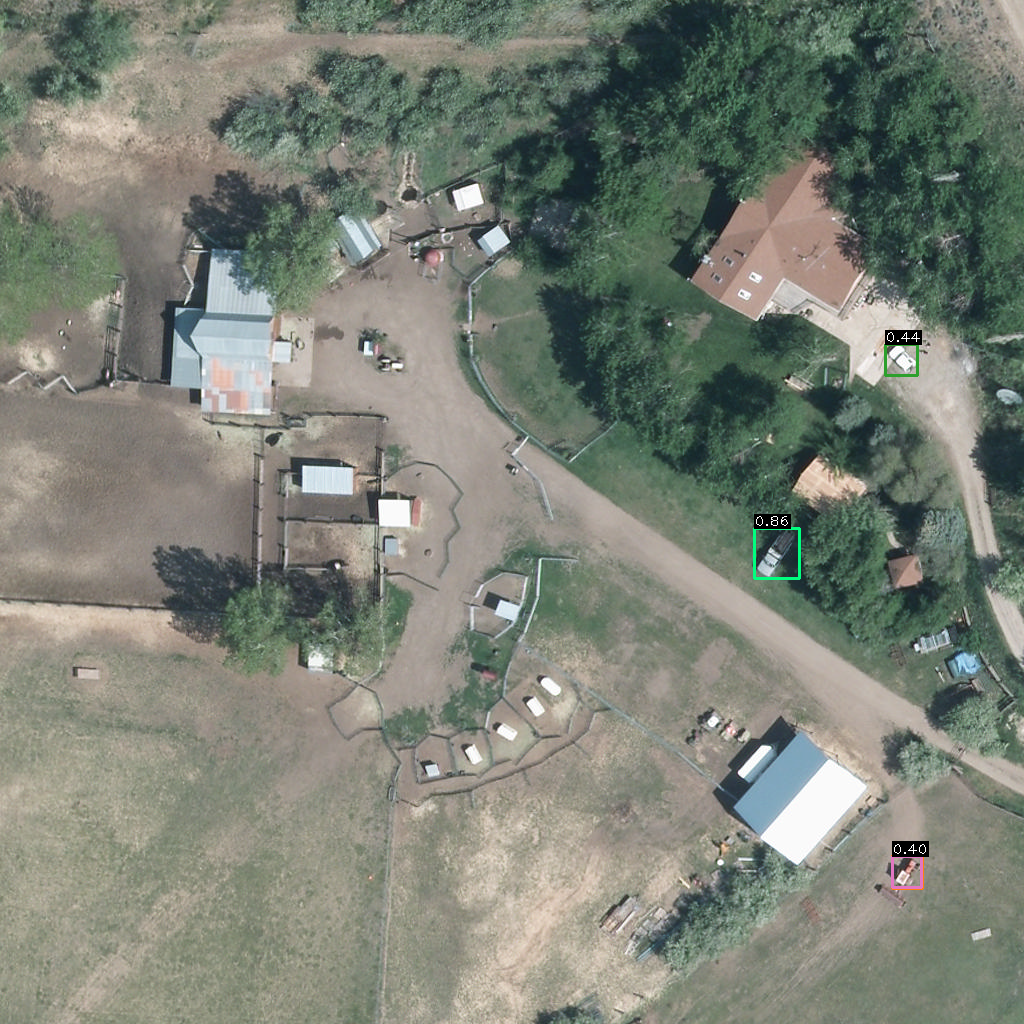
\includegraphics[trim={730pt 220pt 200pt 720pt},clip,width=\linewidth]{images/015Results/01abb_vs_obb/comp_images/abb/523.png}
    %Tractor
    & 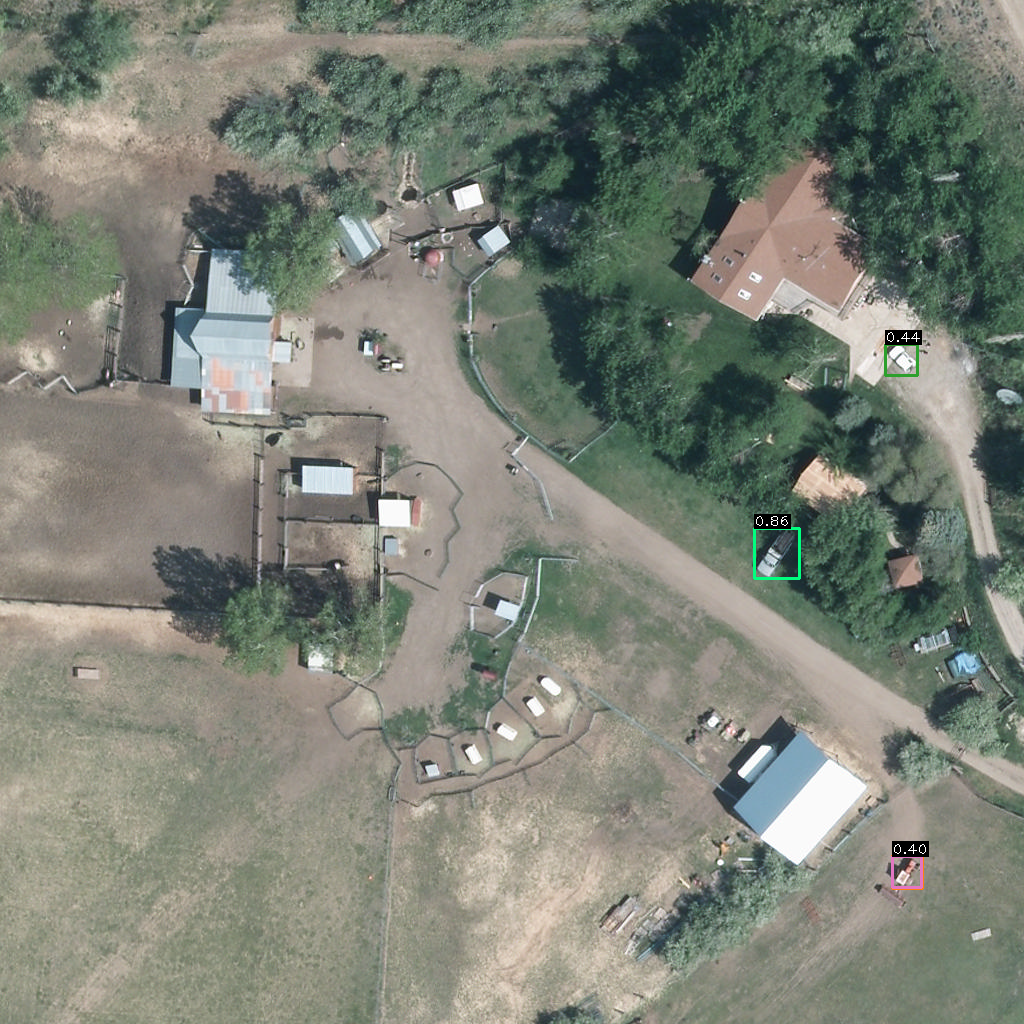
\includegraphics[trim={850pt 110pt 80pt 830pt},clip,width=\linewidth]{images/015Results/01abb_vs_obb/comp_images/abb/523.png}
    %Plane
    &  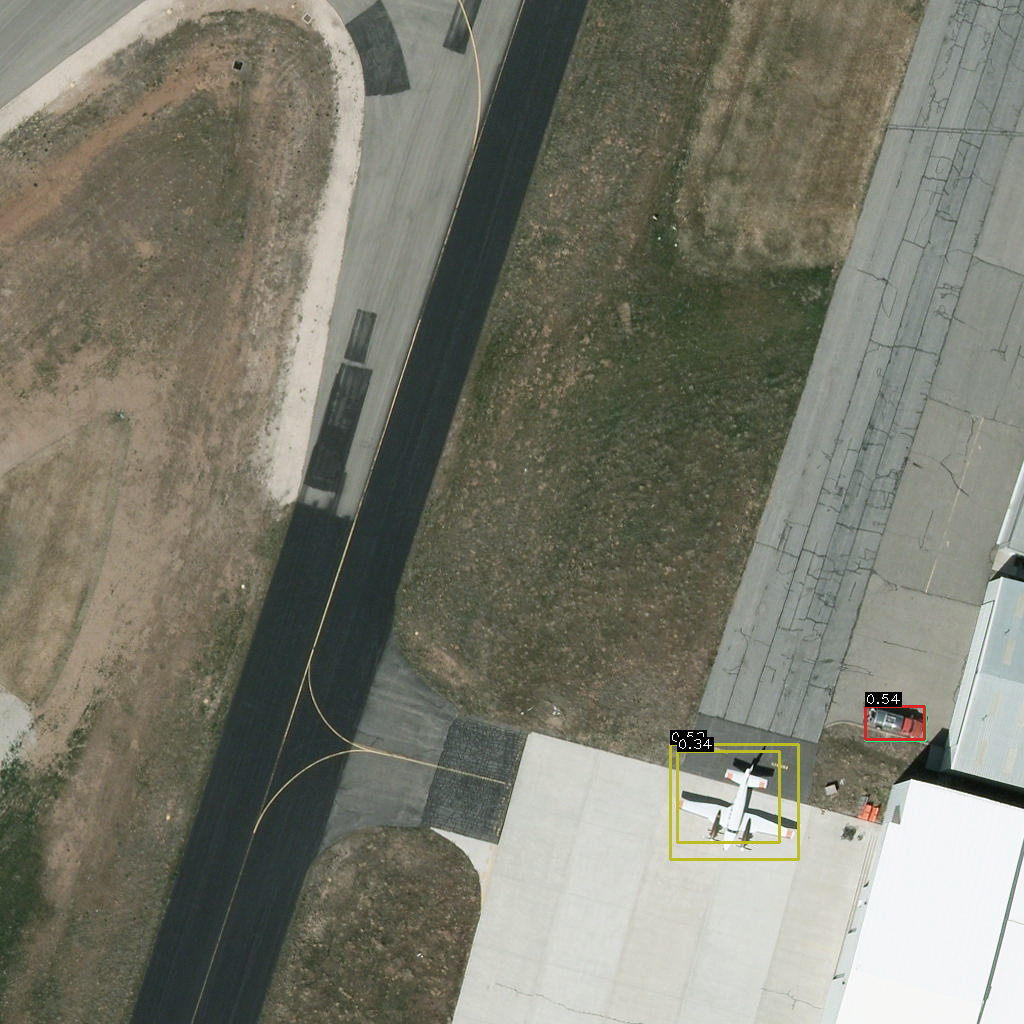
\includegraphics[trim={650pt 120pt 170pt 720pt},clip,width=\linewidth]{images/015Results/01abb_vs_obb/comp_images/abb/487.png}
    %Ship
    & 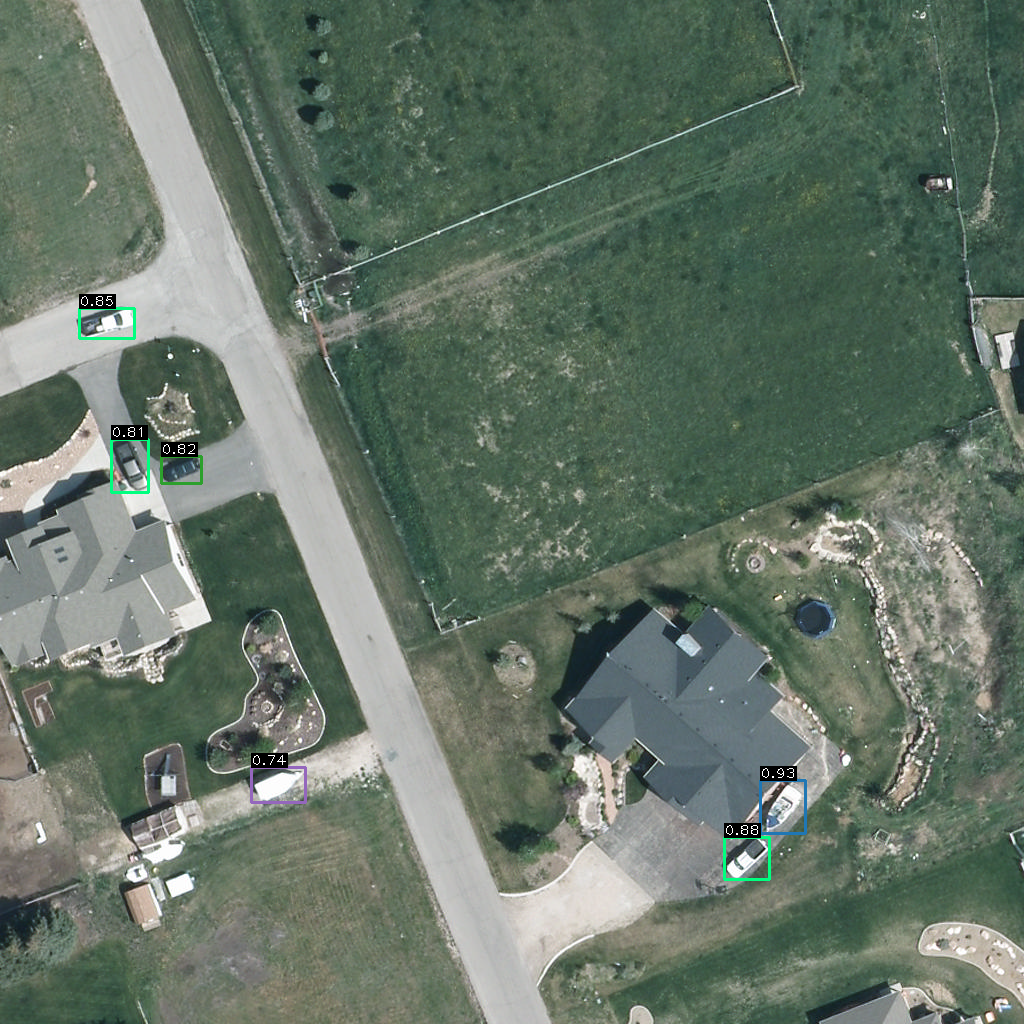
\includegraphics[trim={230pt 200pt 680pt 725pt},clip,width=\linewidth]{images/015Results/01abb_vs_obb/comp_images/abb/509.png}
    %vehicle
    & 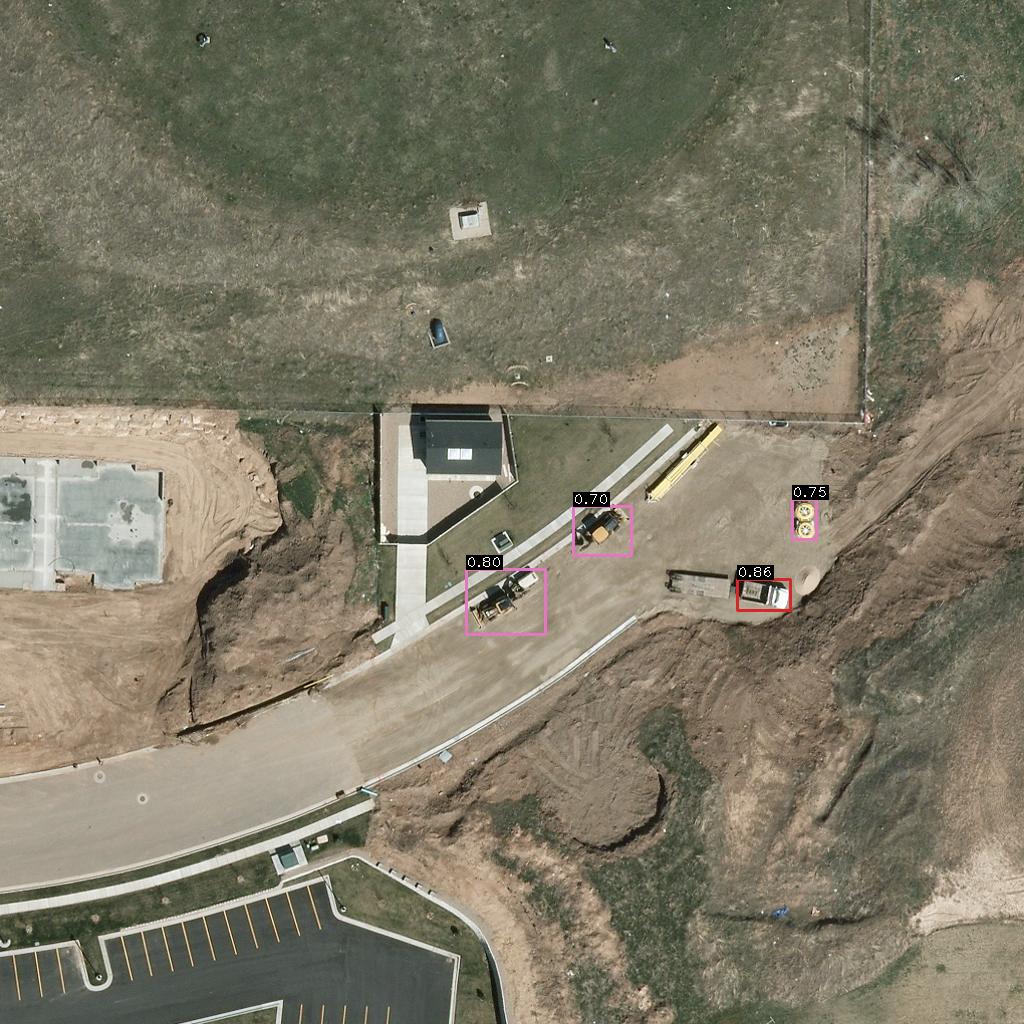
\includegraphics[trim={440pt 360pt 460pt 555pt},clip,width=\linewidth]{images/015Results/01abb_vs_obb/comp_images/abb/427.png}
    %Pick Up
    & 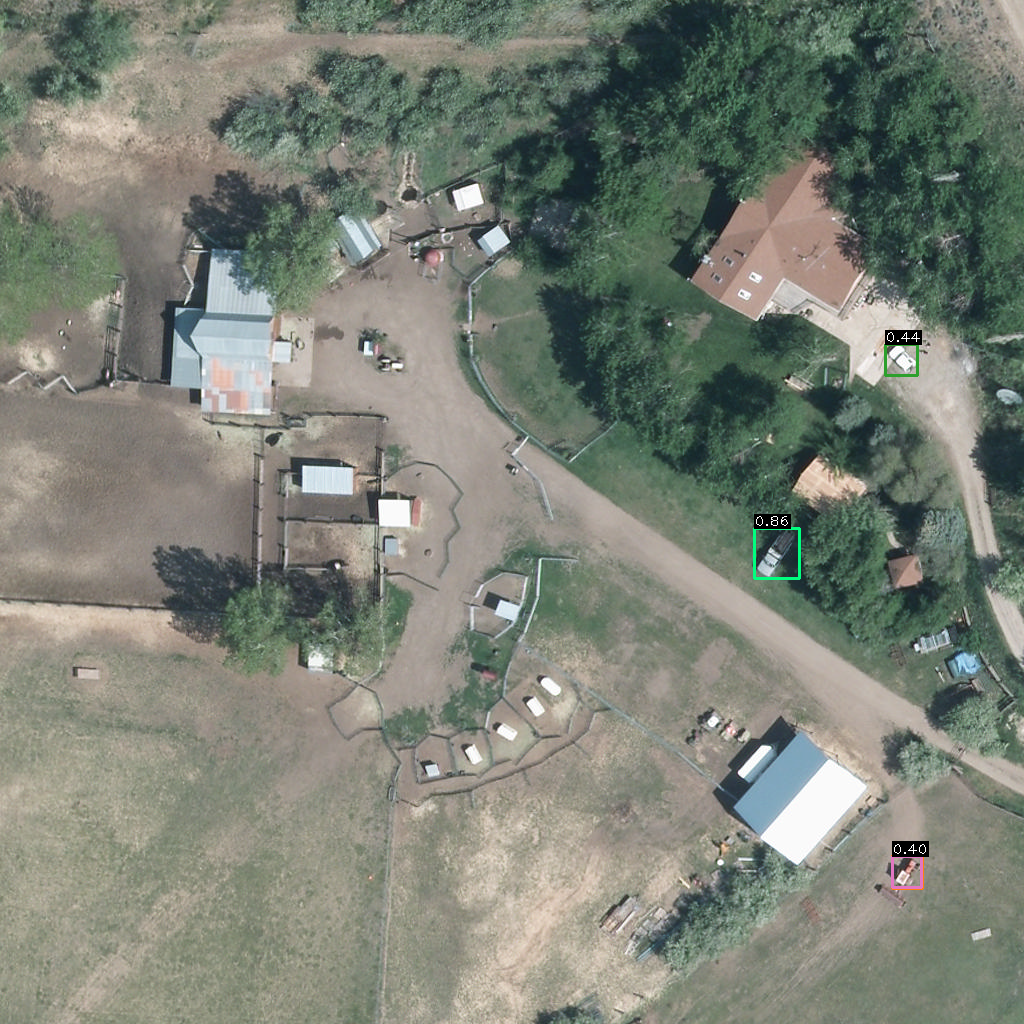
\includegraphics[trim={740pt 420pt 180pt 510pt},clip,width=\linewidth]{images/015Results/01abb_vs_obb/comp_images/abb/523.png}
    %Van
    & 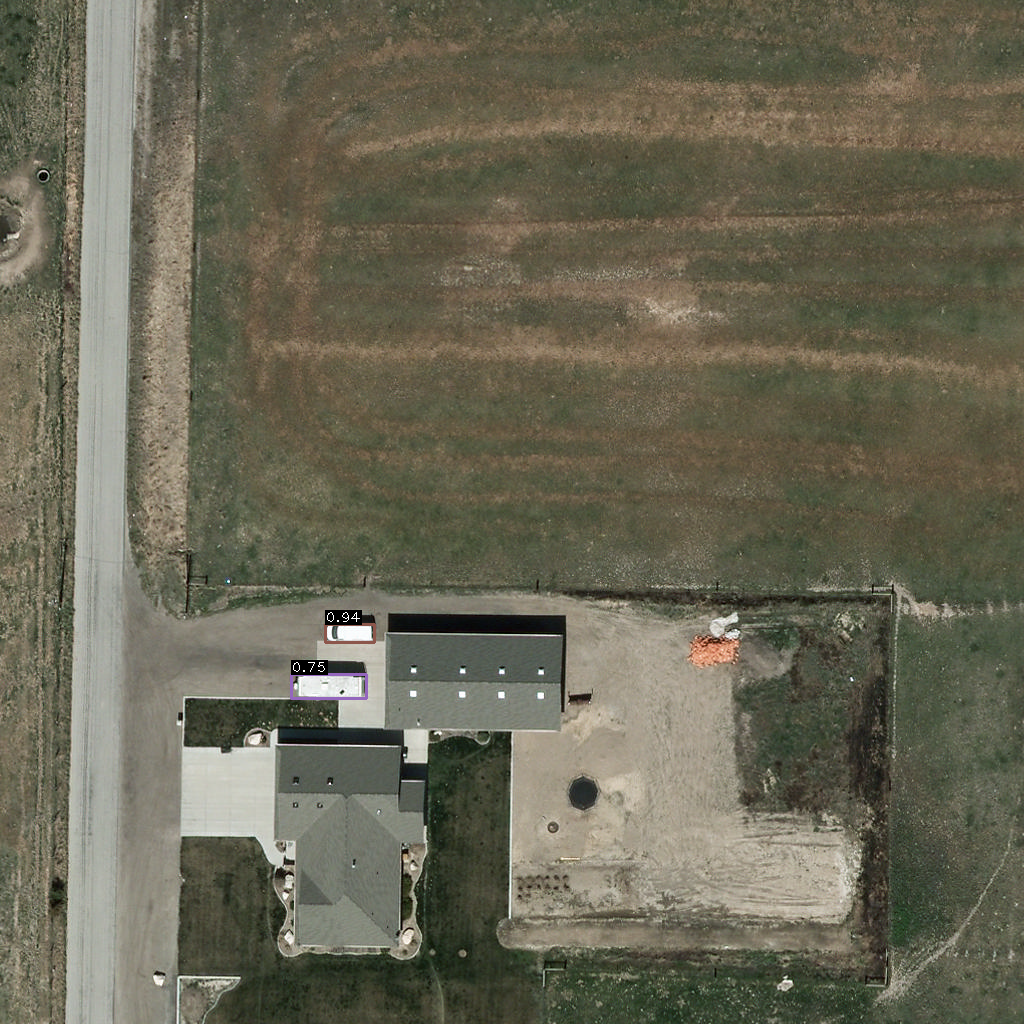
\includegraphics[trim={300pt 355pt 610pt 570pt},clip,width=\linewidth]{images/015Results/01abb_vs_obb/comp_images/abb/198.png} \\ \hline
    \rotatebox{90}{\textbf{\acrshort{obb}}} 
    %Car
    & 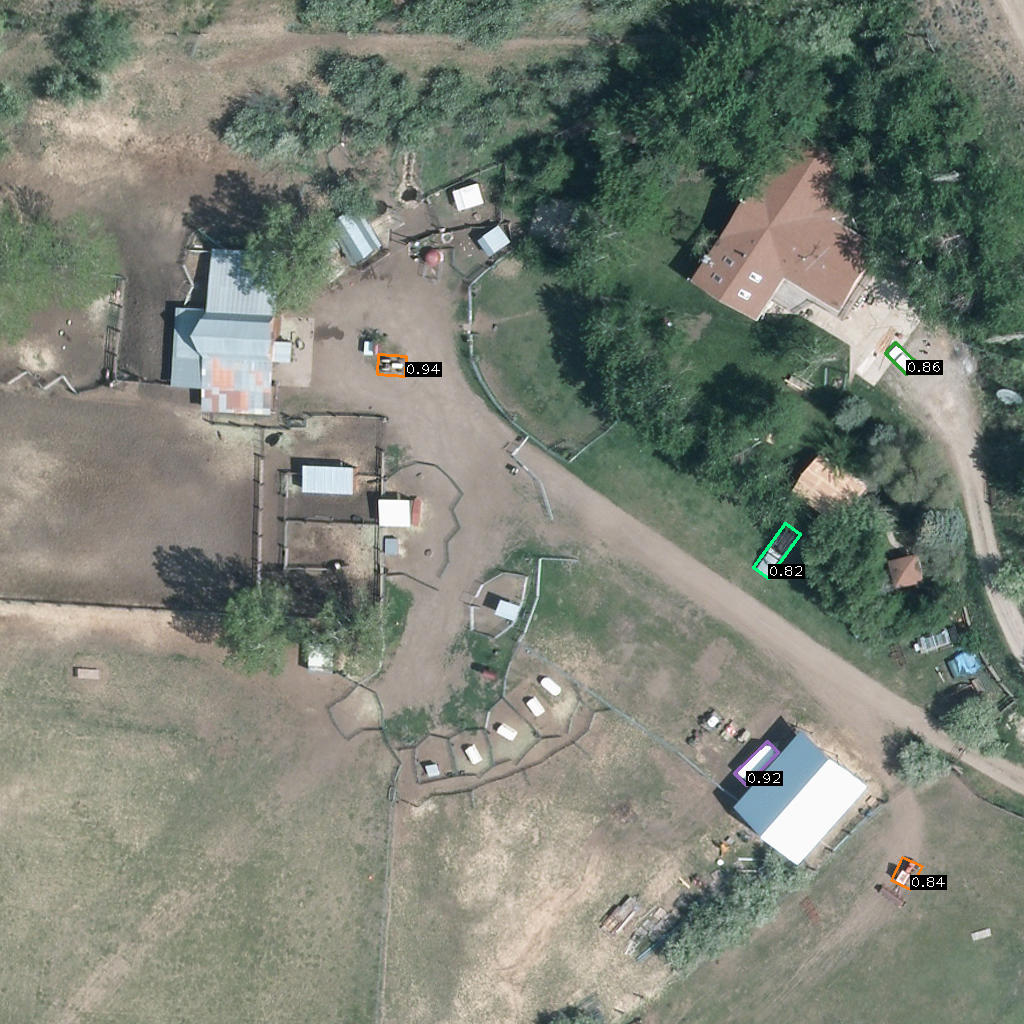
\includegraphics[trim={880pt 630pt 70pt 330pt},clip,width=\linewidth]{images/015Results/01abb_vs_obb/comp_images/obb/523.png}
    %Truck
    & 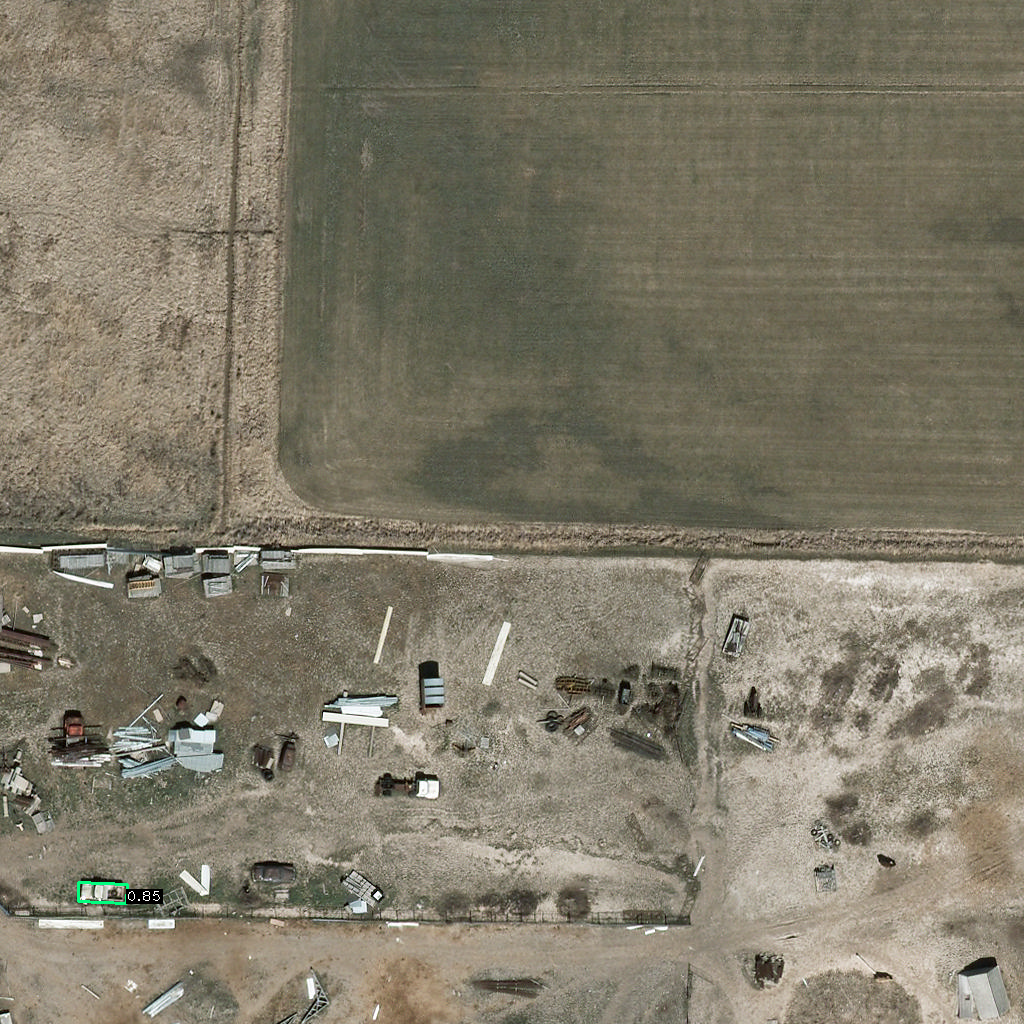
\includegraphics[trim={360pt 200pt 540pt 715pt},clip,width=\linewidth]{images/015Results/01abb_vs_obb/comp_images/obb/212.png}
    %Camping Car
    & 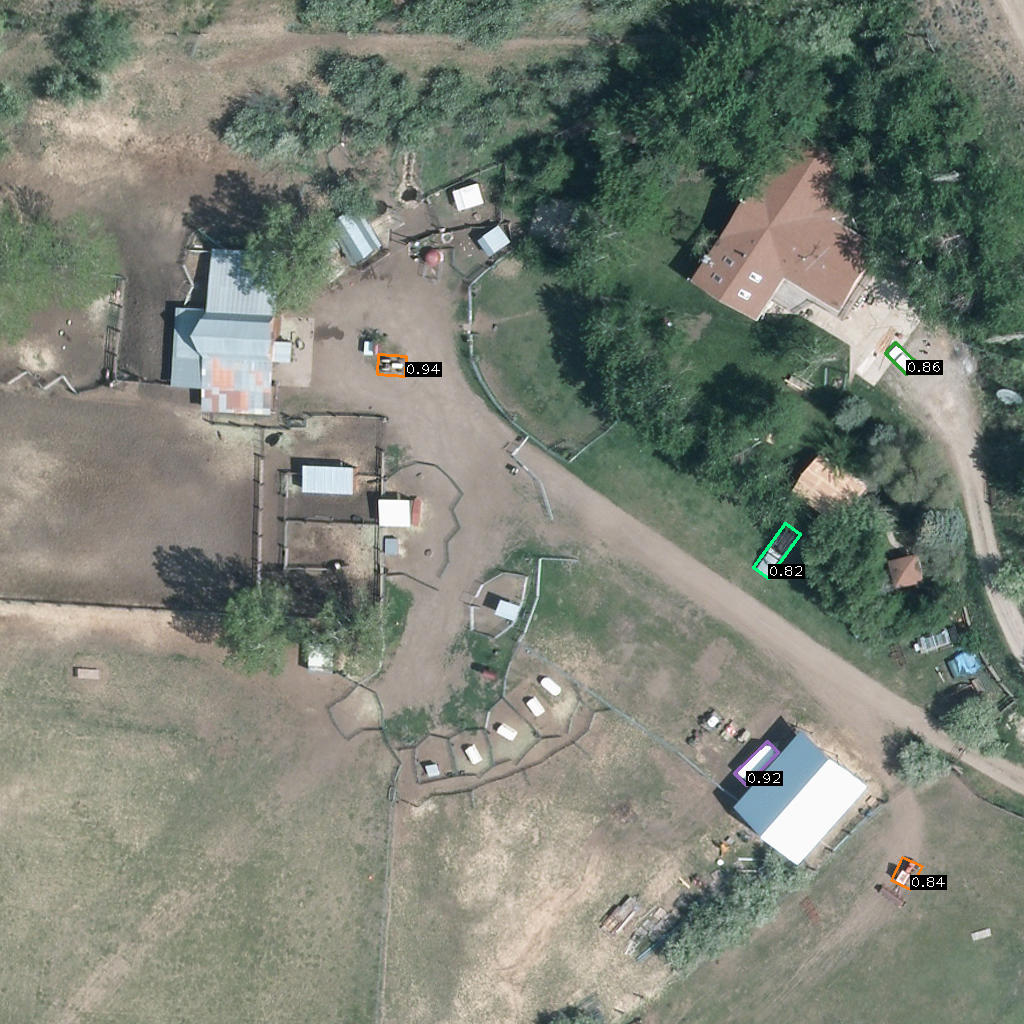
\includegraphics[trim={730pt 220pt 200pt 720pt},clip,width=\linewidth]{images/015Results/01abb_vs_obb/comp_images/obb/523.png}
    %Tractor
    & 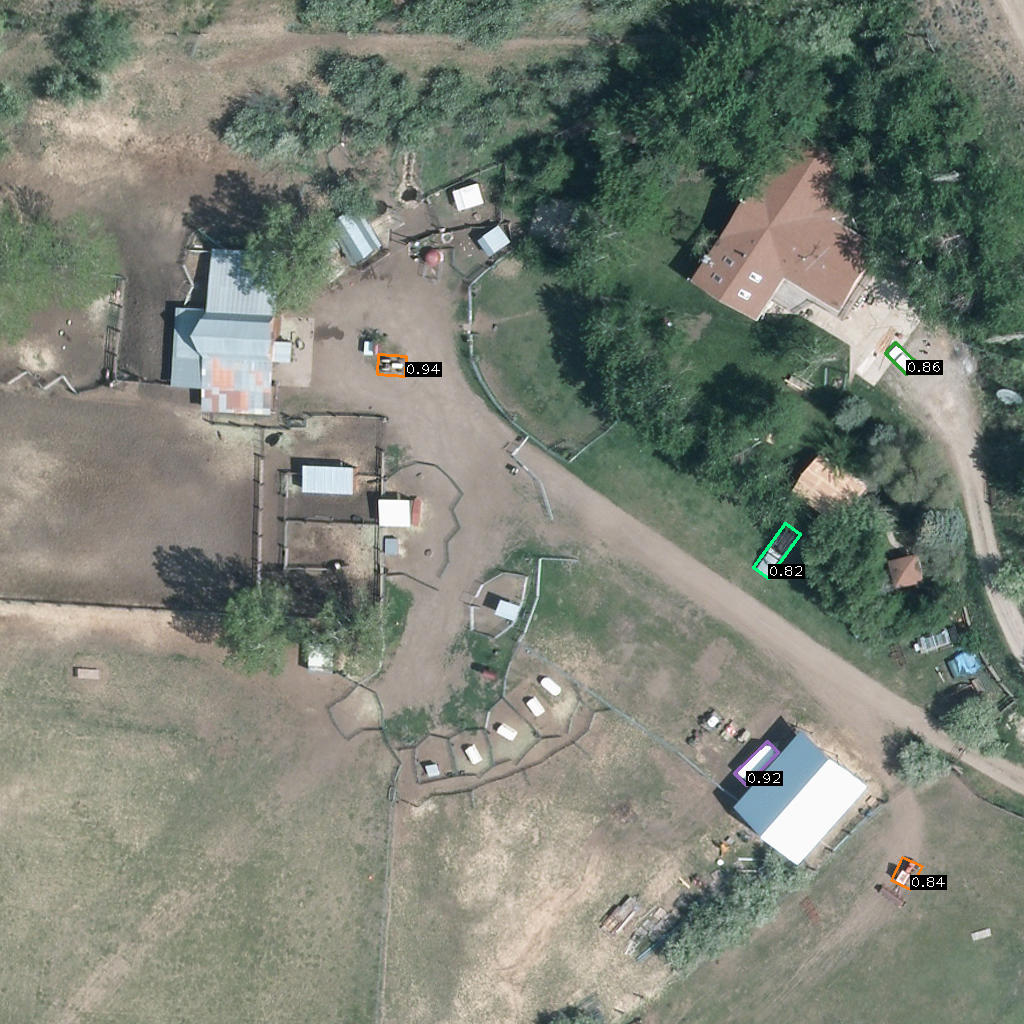
\includegraphics[trim={850pt 110pt 80pt 830pt},clip,width=\linewidth]{images/015Results/01abb_vs_obb/comp_images/obb/523.png}
    %Plane
    &  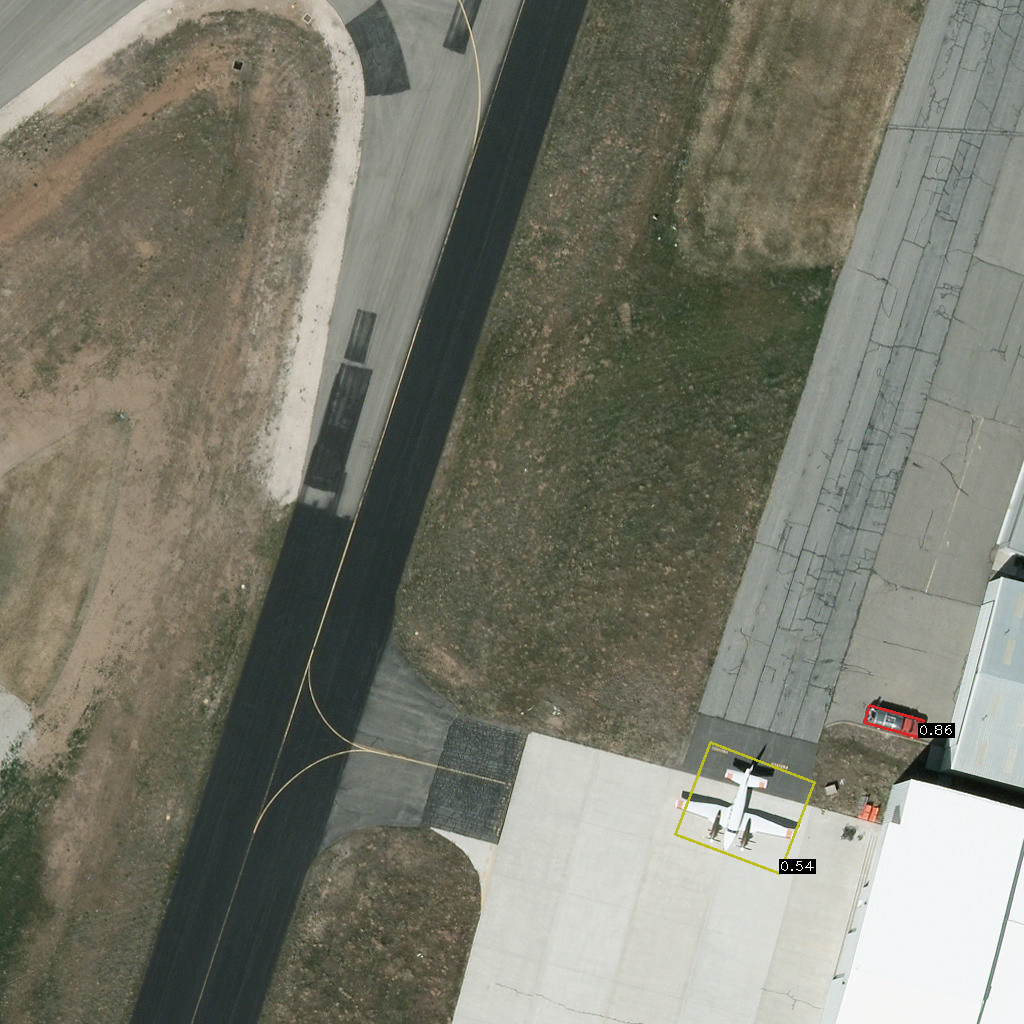
\includegraphics[trim={650pt 120pt 170pt 720pt},clip,width=\linewidth]{images/015Results/01abb_vs_obb/comp_images/obb/487.png}
    %Ship
    & 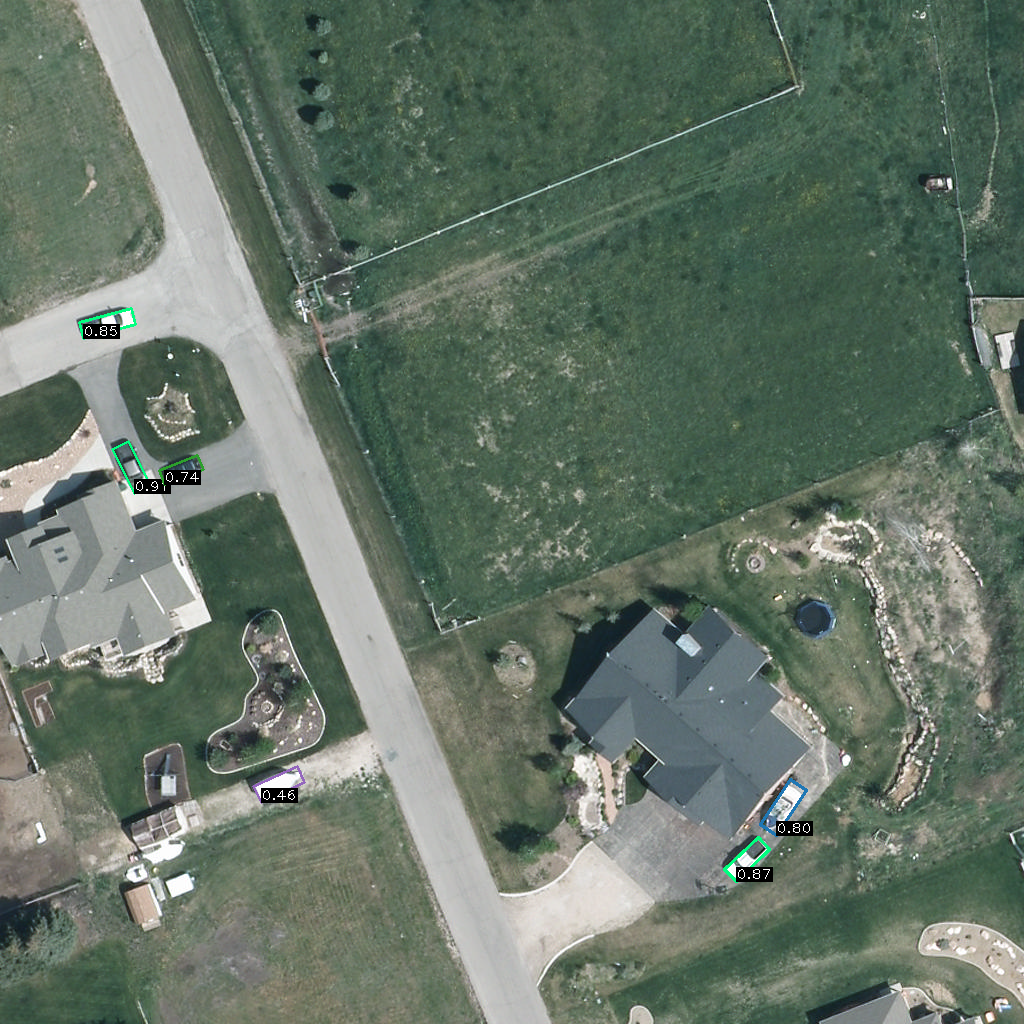
\includegraphics[trim={230pt 200pt 680pt 725pt},clip,width=\linewidth]{images/015Results/01abb_vs_obb/comp_images/obb/509.png}
    %vehicle
    & 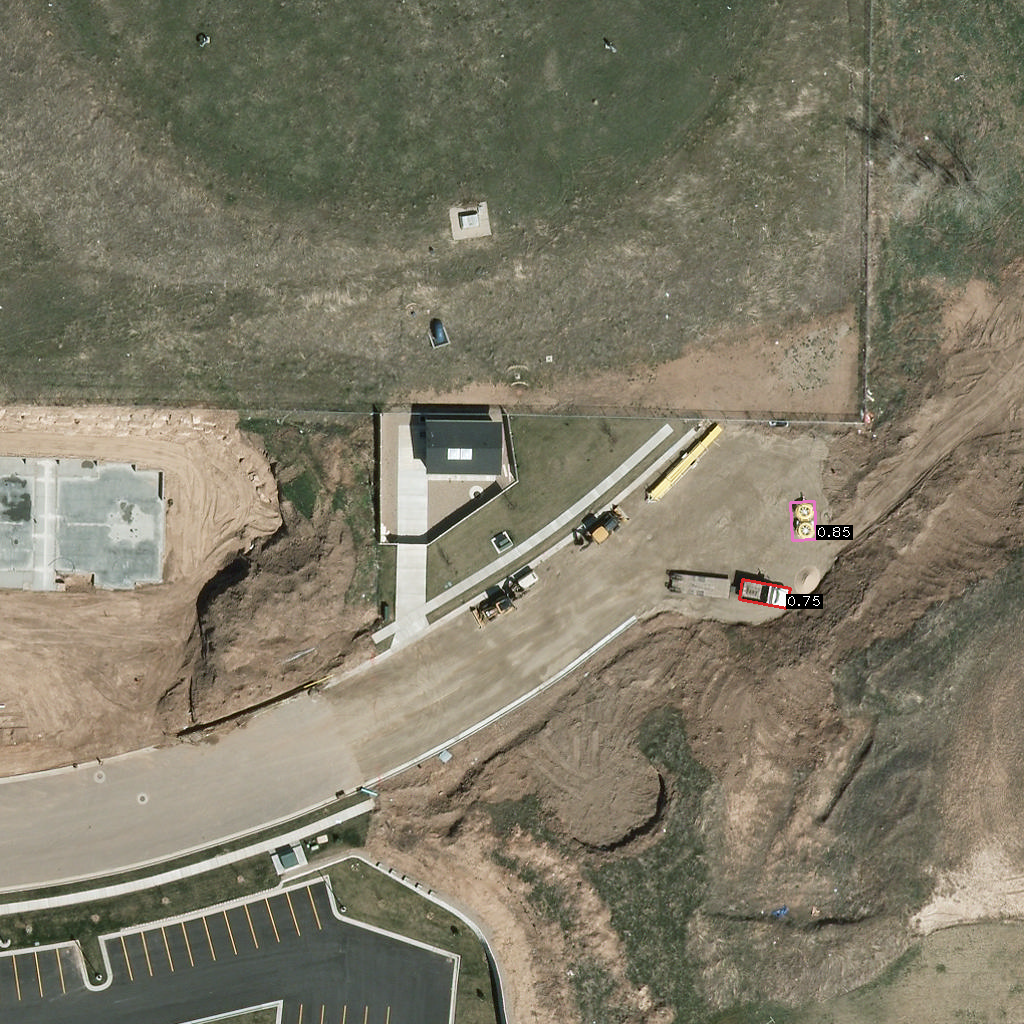
\includegraphics[trim={440pt 360pt 460pt 555pt},clip,width=\linewidth]{images/015Results/01abb_vs_obb/comp_images/obb/427.png}
    %Pick Up
    & 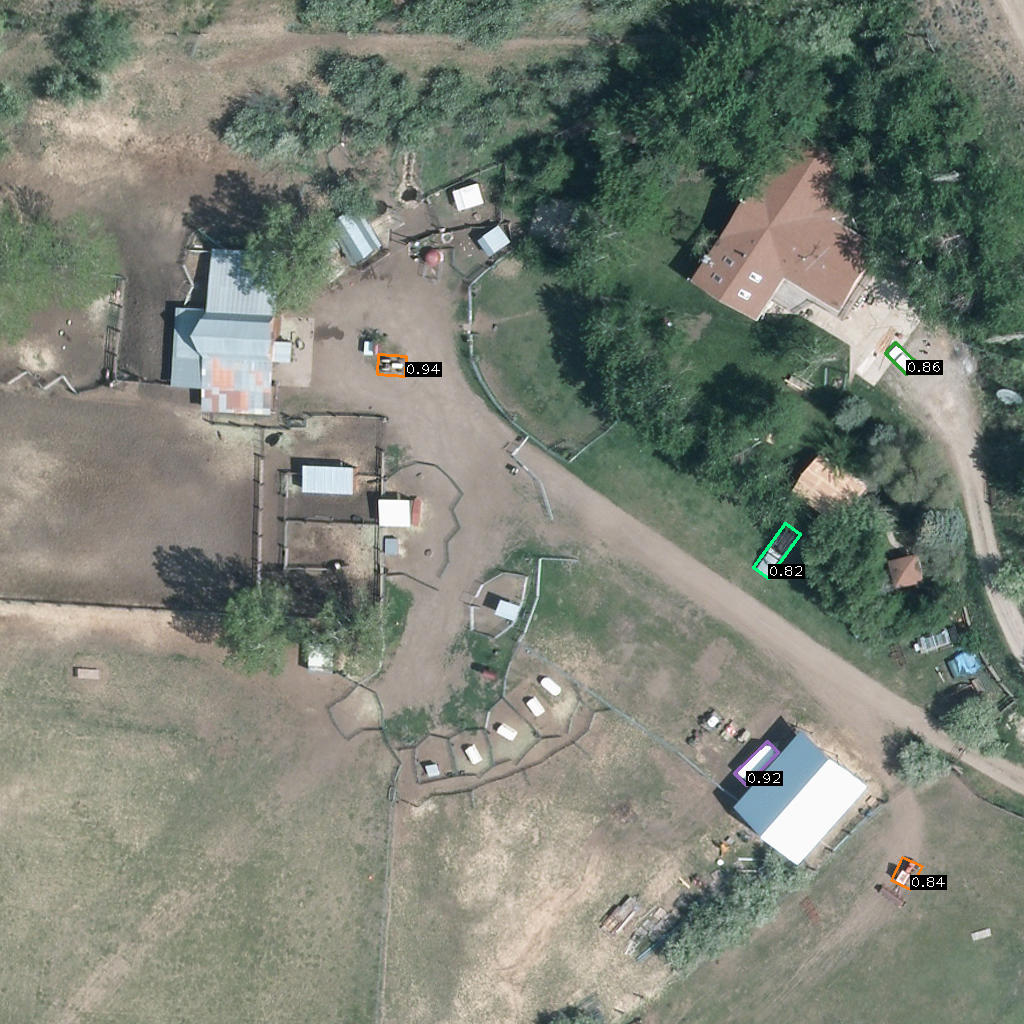
\includegraphics[trim={740pt 420pt 180pt 510pt},clip,width=\linewidth]{images/015Results/01abb_vs_obb/comp_images/obb/523.png}
    %Van
    & 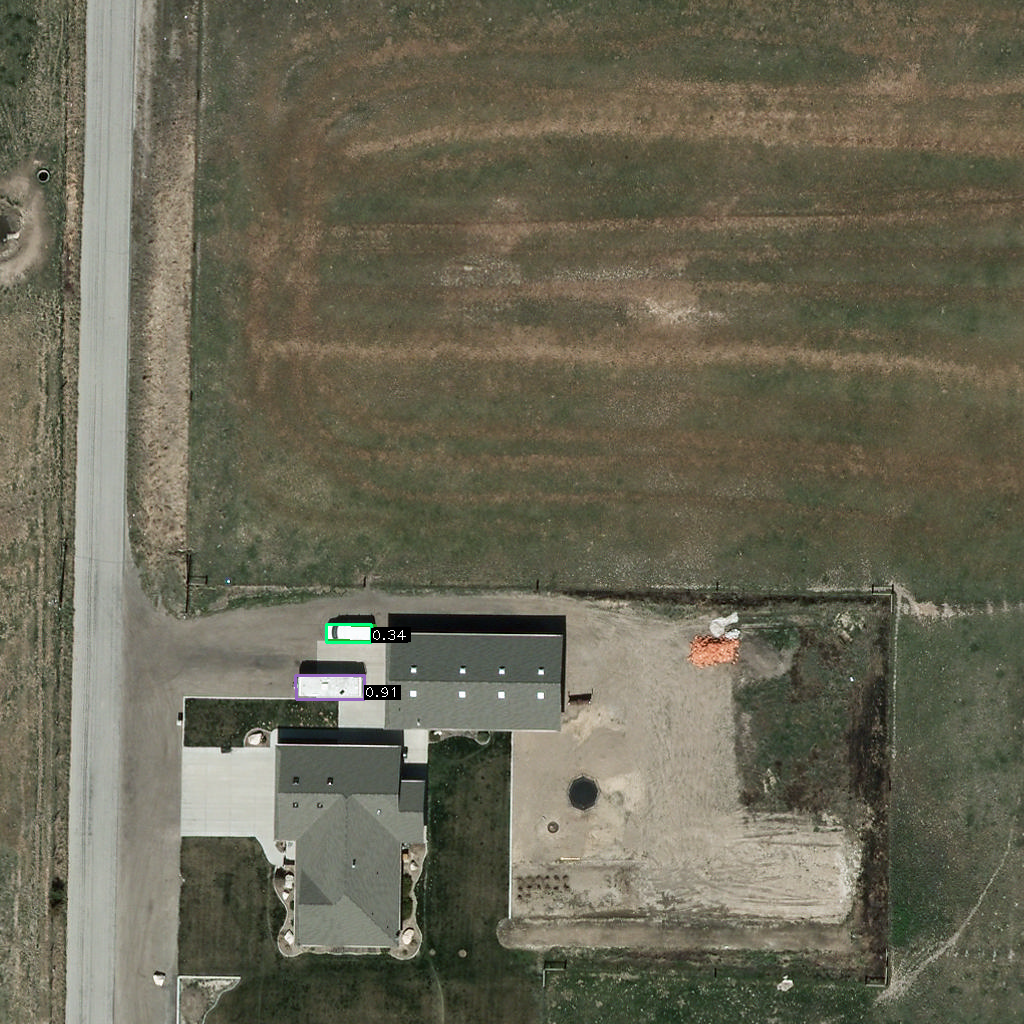
\includegraphics[trim={300pt 355pt 610pt 570pt},clip,width=\linewidth]{images/015Results/01abb_vs_obb/comp_images/obb/198.png} \\ \hline
     \rotatebox{90}{\textbf{\acrshort{abb} in \acrshort{obb}}} 
    %Car
    & 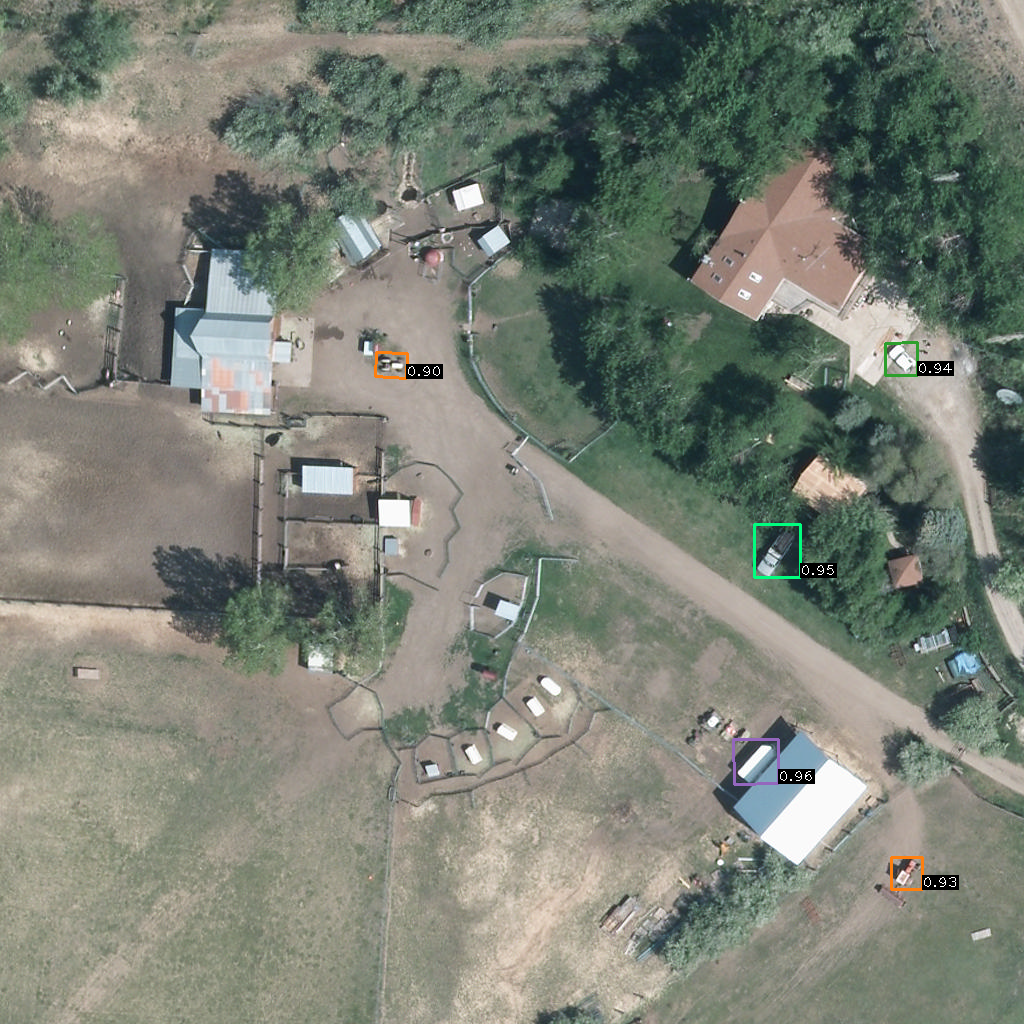
\includegraphics[trim={880pt 630pt 70pt 330pt},clip,width=\linewidth]{images/015Results/01abb_vs_obb/comp_images/aab_old/523.png}
    %Truck
    & 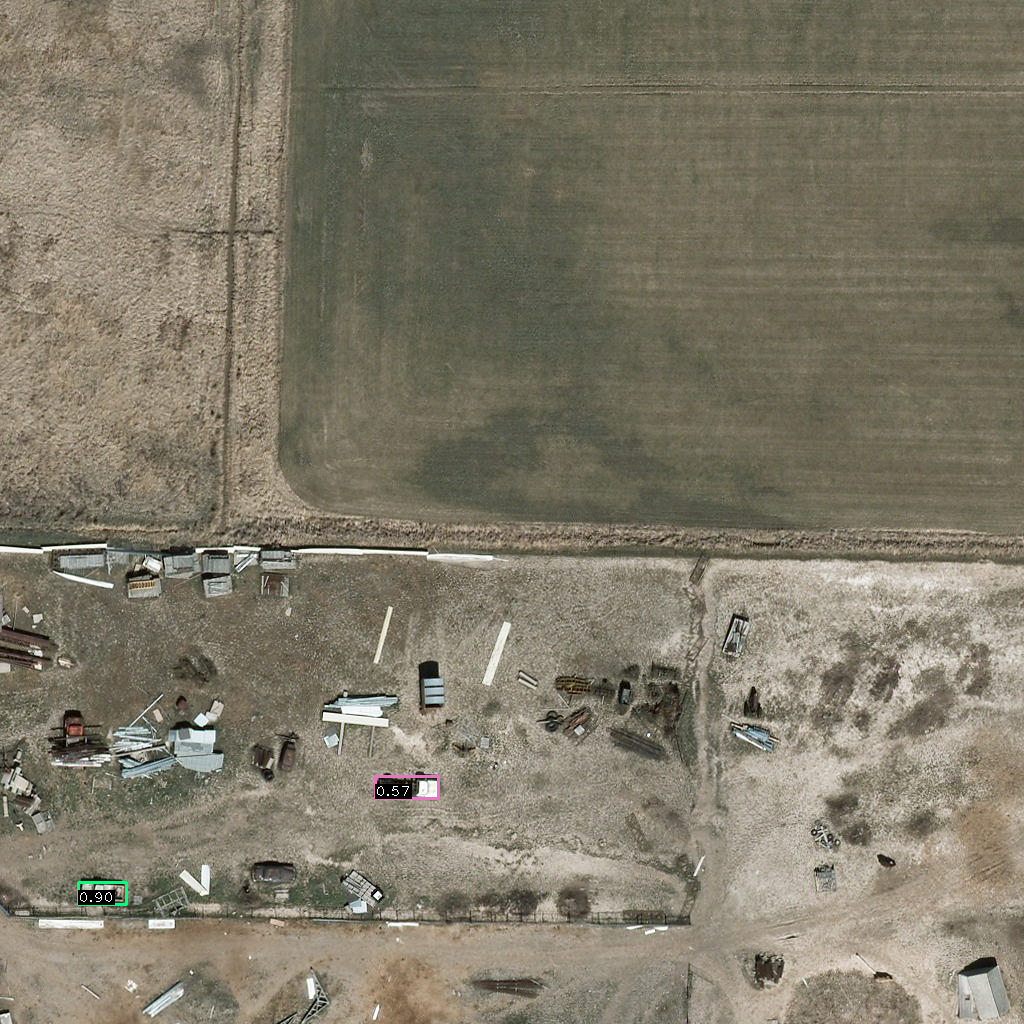
\includegraphics[trim={360pt 200pt 540pt 715pt},clip,width=\linewidth]{images/015Results/01abb_vs_obb/comp_images/aab_old/212.png}
    %Camping Car
    & 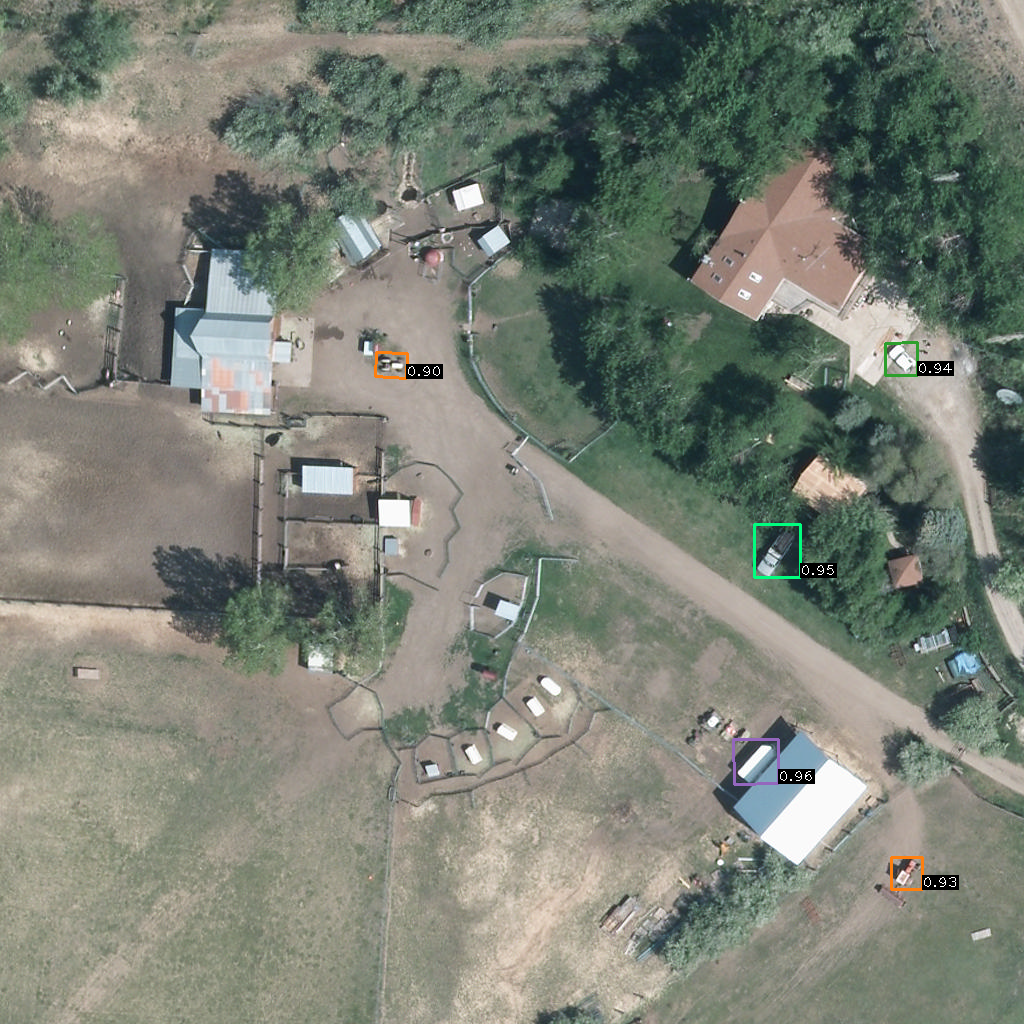
\includegraphics[trim={730pt 220pt 200pt 720pt},clip,width=\linewidth]{images/015Results/01abb_vs_obb/comp_images/aab_old/523.png}
    %Tractor
    & 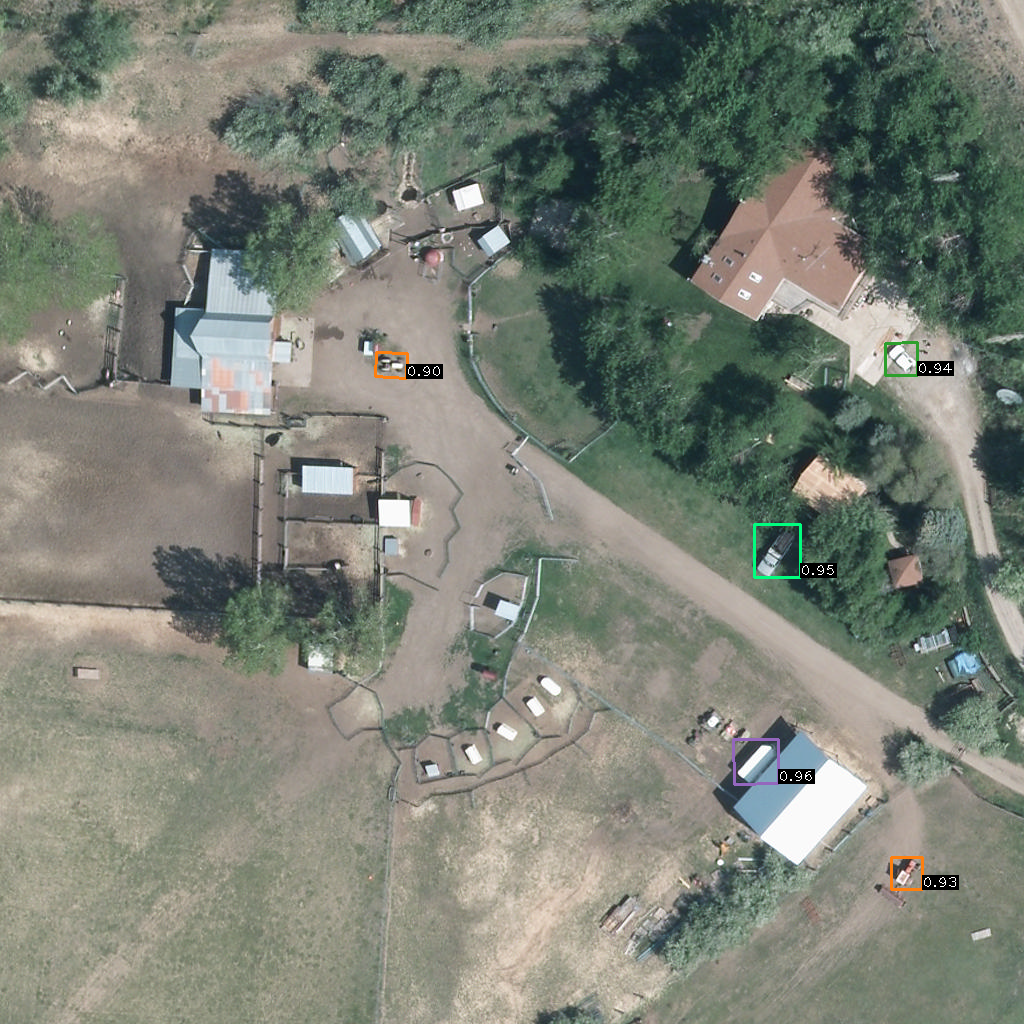
\includegraphics[trim={850pt 110pt 80pt 830pt},clip,width=\linewidth]{images/015Results/01abb_vs_obb/comp_images/aab_old/523.png}
    %Plane
    &  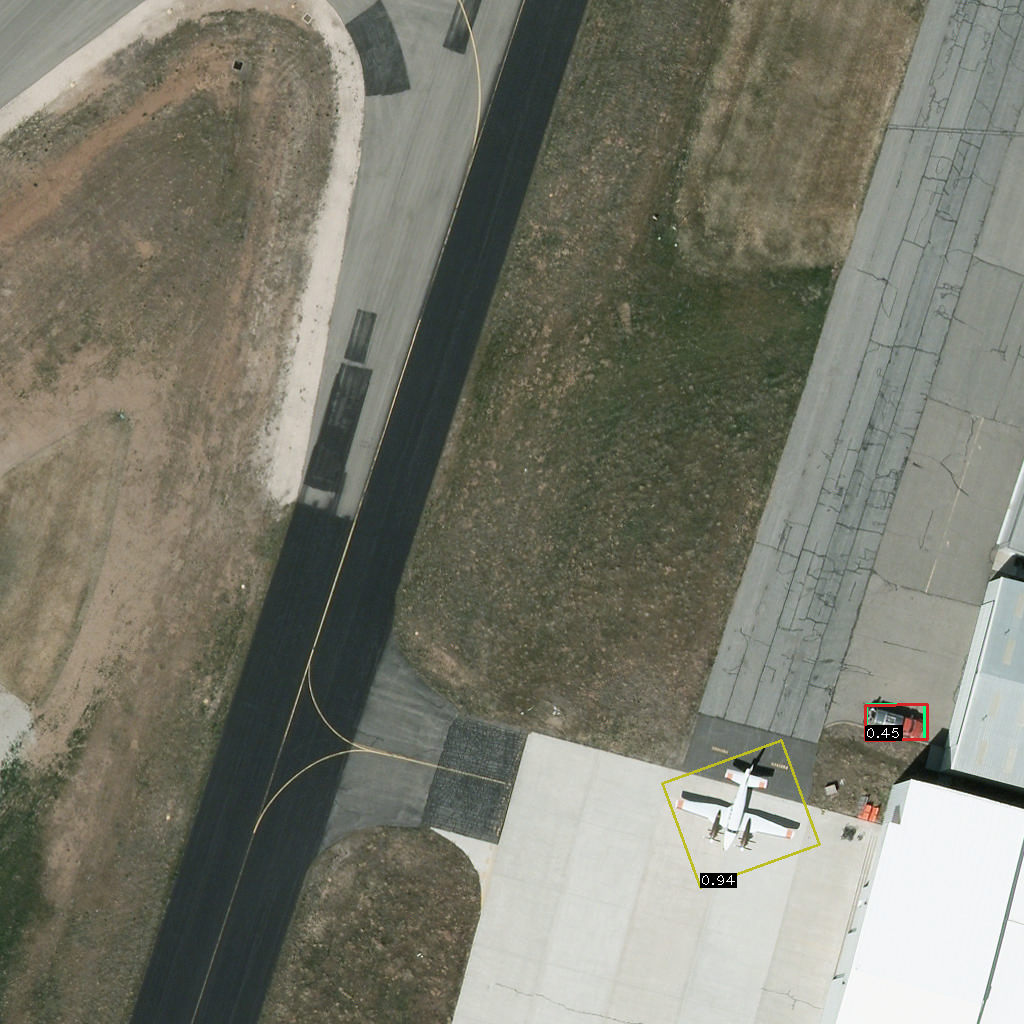
\includegraphics[trim={650pt 120pt 170pt 720pt},clip,width=\linewidth]{images/015Results/01abb_vs_obb/comp_images/aab_old/487.png}
    %Ship
    & 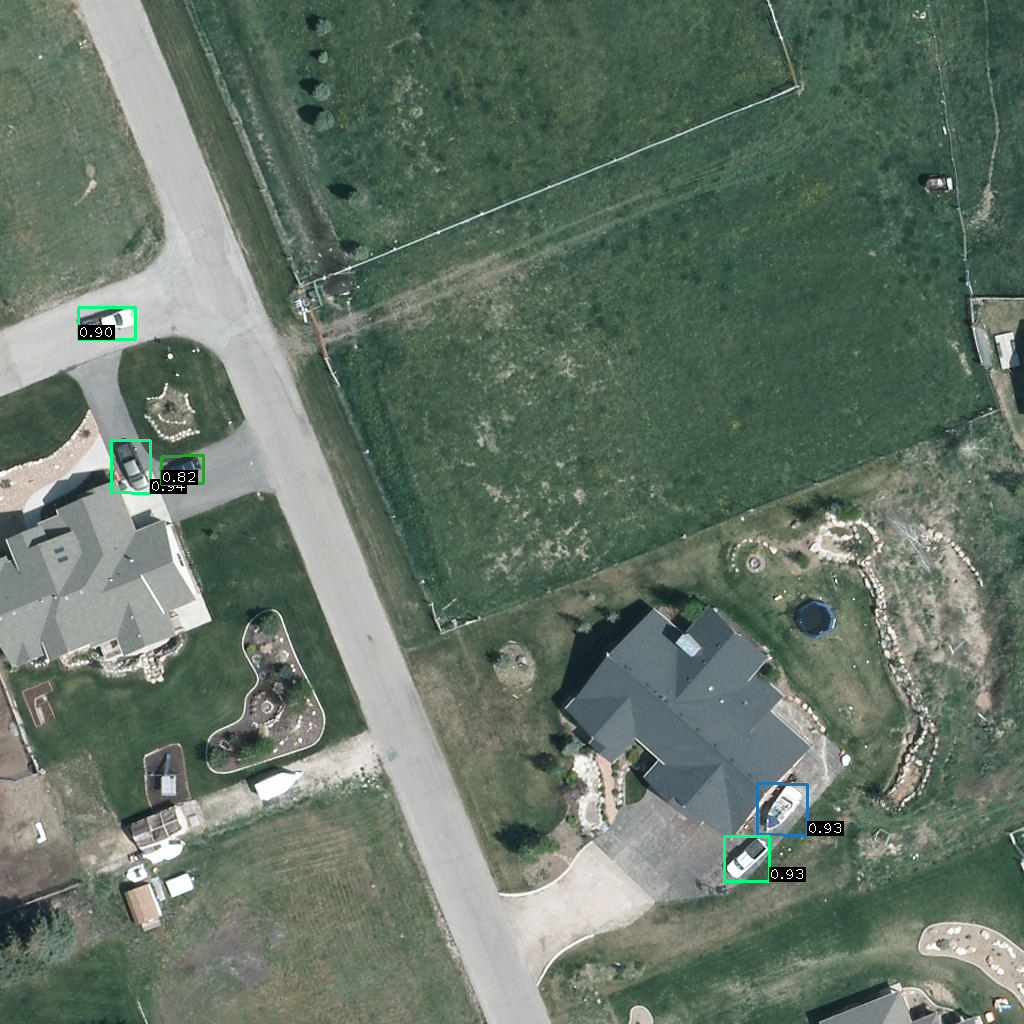
\includegraphics[trim={230pt 200pt 680pt 725pt},clip,width=\linewidth]{images/015Results/01abb_vs_obb/comp_images/aab_old/509.png}
    %vehicle
    & 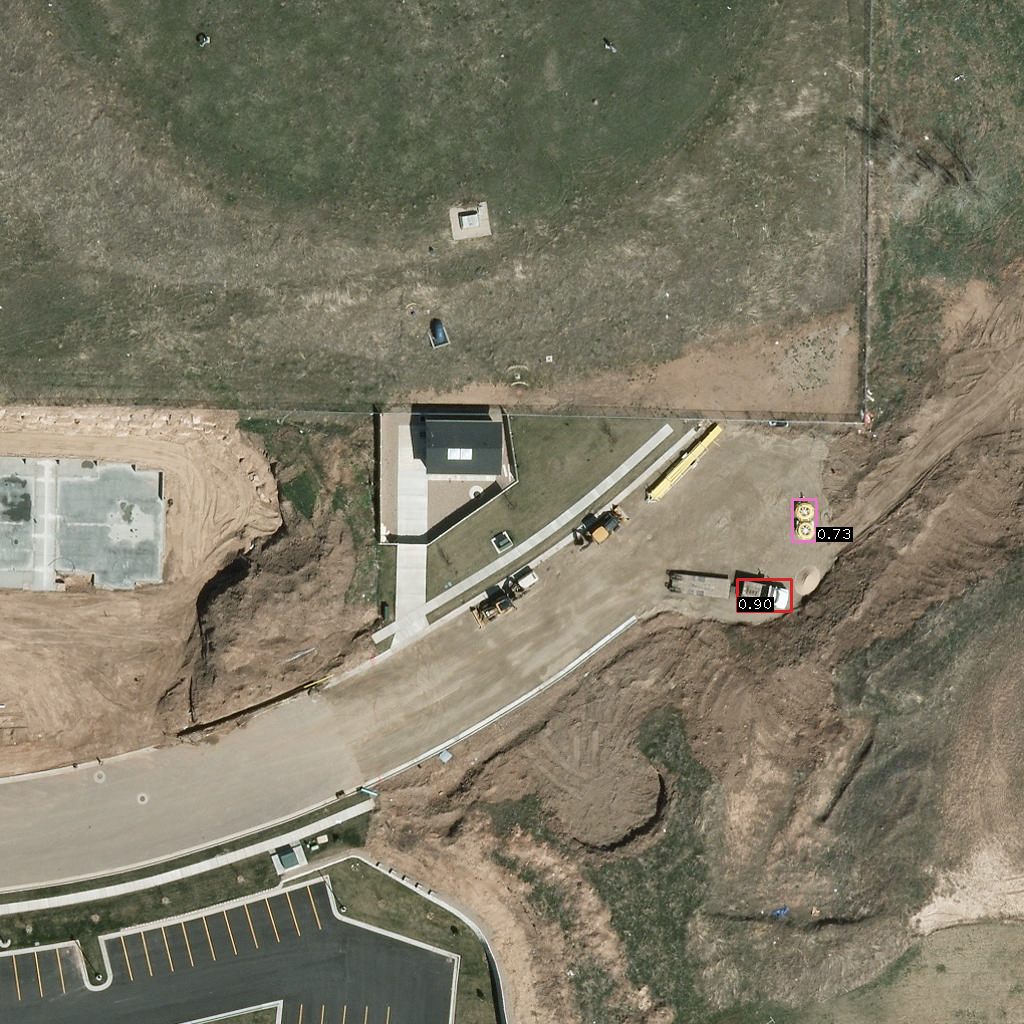
\includegraphics[trim={440pt 360pt 460pt 555pt},clip,width=\linewidth]{images/015Results/01abb_vs_obb/comp_images/aab_old/427.png}
    %Pick Up
    & 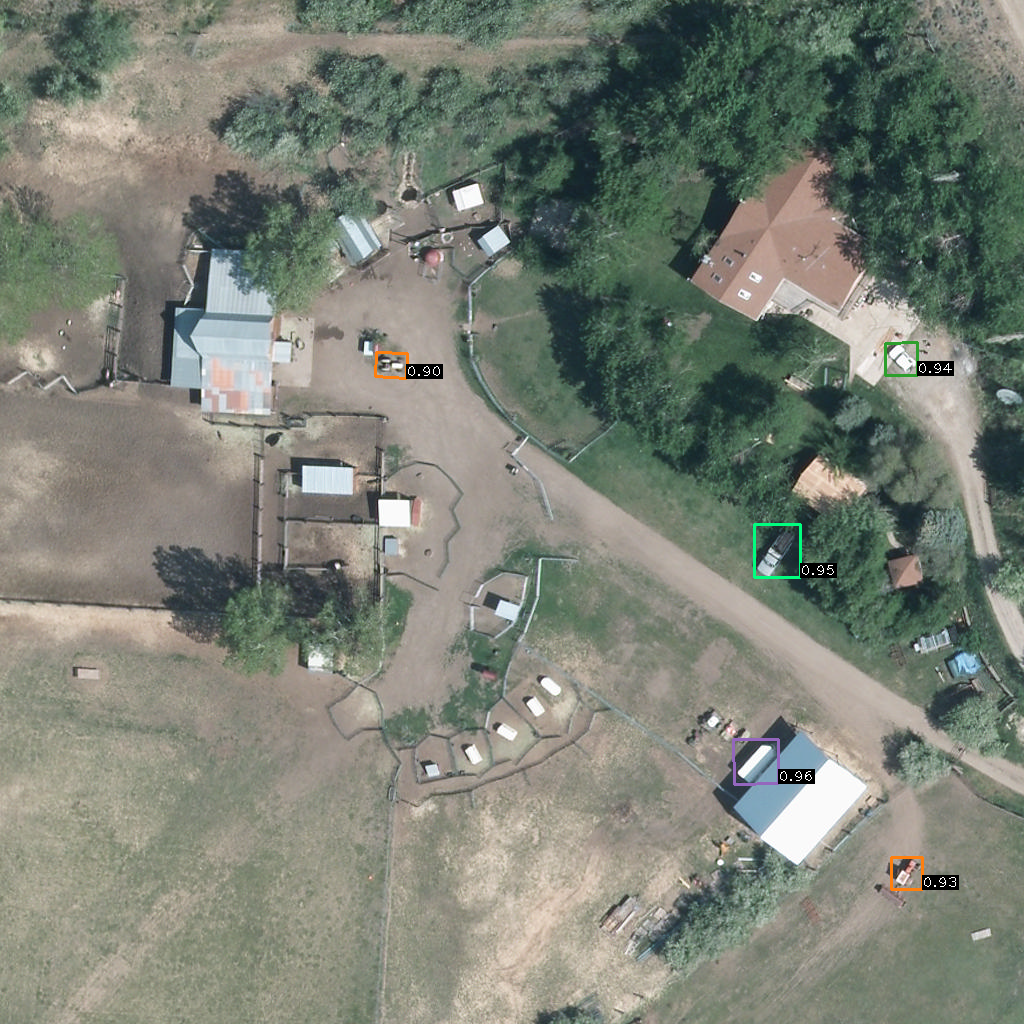
\includegraphics[trim={740pt 420pt 180pt 510pt},clip,width=\linewidth]{images/015Results/01abb_vs_obb/comp_images/aab_old/523.png}
    %Van
    & 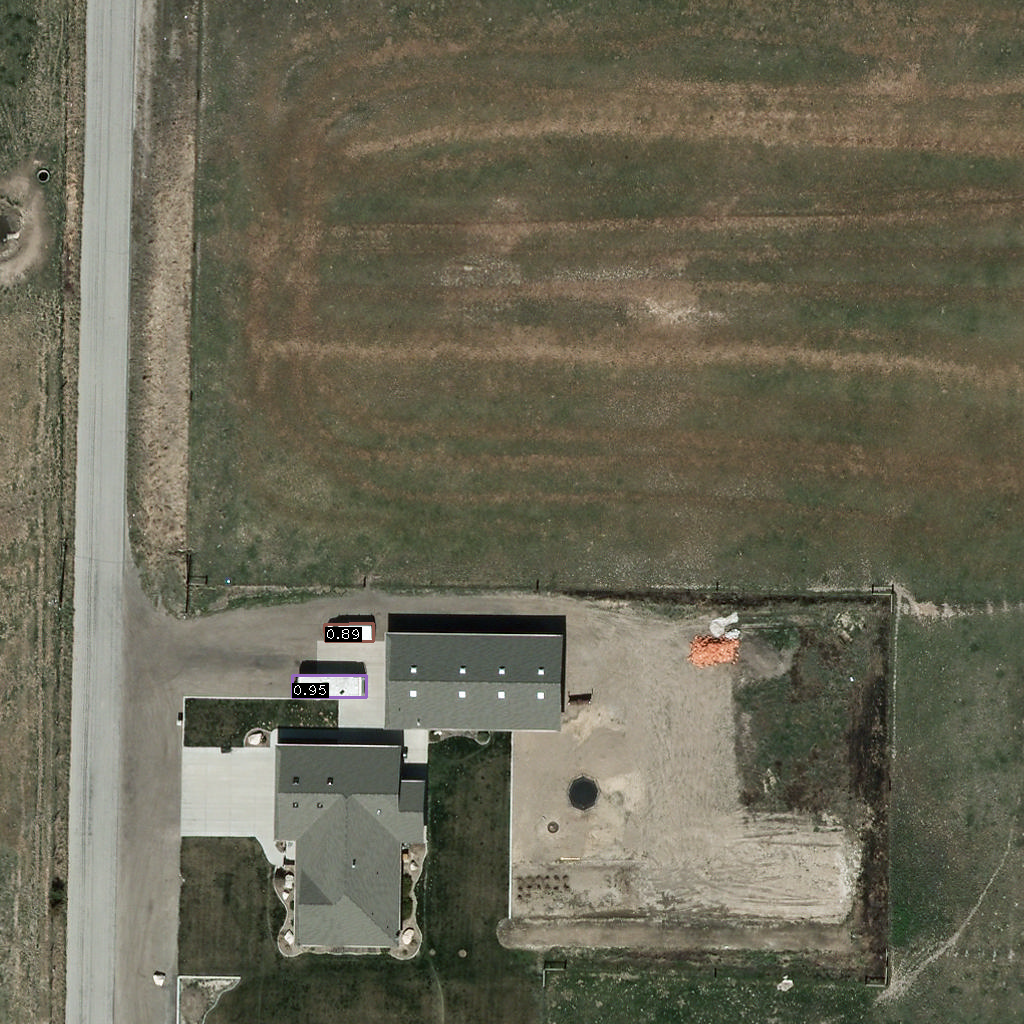
\includegraphics[trim={300pt 355pt 610pt 570pt},clip,width=\linewidth]{images/015Results/01abb_vs_obb/comp_images/aab_old/198.png} \\ \hline
\end{tabularx}
\caption[aab and obb: Examples of different classes for the object recognition performance]{Examples of different classes for the object recognition performance of different bounding box formats. The numbers displayed on the bounding boxes indicate the confidence of the model in the classification of the respective box. For Color Scheme explanation see Tab. \ref{tab:class_colors}}.
\label{fig:aab_obb_example_pics}
\end{figure}

%##########################################################################
%##########################################################################






\FloatBarrier
%##########################################################################
%##########################################################################
%##########################################################################
%##########################################################################
%##########################################################################
%##########################################################################
%##########################################################################
%##########################################################################
%##########################################################################

\section{Permutation Experiments}
\begin{figure}[t]
    \centering
    \includesvg[width=0.9\textwidth]{images/015Results/02perm_exp/perm_exp_best_val_on_test.svg}
    \caption[Comparison of \acrshort{mAP}@0.5--0.95 values for different channel permutation models (Best validation model on test dataset)]{Comparison of \acrshort{mAP}@0.5--0.95 values for different channel permutation models (Best validation model on test dataset). The red dot is the fold, that has the best \acrshort{mAP}@0.5--0.95 at the validation dataset (see fig. \ref{fig:perm_exp_map50-95:val_on_val}). \acrshort{RGIR} performs best, with models using \acrshort{NDVI} performing significantly worse than the five main permutations. \acrshort{NDVI} may introduce noise. Fluctuations between the quantiles in the main permutations are due to the fact that the channel changes do have an influence. \acrshort{RGBIR} has the third-best performance because it contains all bands. \acrshort{RGB} and \acrshort{RIRB} are better, possibly because too much information also causes noise (Own representation).}
    \label{fig:perm_exp_map50-95:val_on_test}
\end{figure}

\begin{figure}[b]
    \centering
    \includesvg[width=0.9\textwidth]{images/015Results/02perm_exp/perm_exp_best_val_on_val.svg}
    \caption[Comparison of \acrshort{mAP}@0.5--0.95 values for different channel permutation models (Best validation model on validation dataset)]{Comparison of \acrshort{mAP}@0.5--0.95 values for different channel permutation models (Best validation model on validation dataset). The RGBIR channel permutation achieves the best performance, followed by the other main permutations, while RGIR performs worst among the five main permutations. Models with NDVI are again significantly worse due to additional noise. The small fluctuations between the five main quantiles indicate robust folds and stable training (Own representation).}
    \label{fig:perm_exp_map50-95:val_on_val}
\end{figure}
The following section first describes the general results of the models in terms of detection performance and compares them with the \acrshort{mAP}@0.5--0.95 values shown in Figure \ref{fig:perm_exp_map50-95:val_on_test}. This is followed by a detailed analysis of class recognition performance using the difference matrices.  

Figure \ref{fig:perm_exp_map50-95:val_on_test} shows that the RGIR model achieves the best \acrshort{mAP}@0.5--0.95 performance on the test fold, followed by the RIRB and RGB models. The comparatively large differences between the quantiles are striking, indicating a greater dispersion of the results. The RGBIR model ranks fourth, while the IRGB model performs significantly weaker than the aforementioned models, but still achieves better results than the two models that include an NDVI channel. The latter show the weakest overall performance, suggesting that the NDVI channel is of limited use for this task. \todo{is actually analysis} 

Comparing the results with those on the validation dataset (see Figure \ref{fig:perm_exp_map50-95:val_on_val}), there are greater fluctuations between the quantiles overall. While the results of most models are close together in the validation data set and only the NDVI-based models show clear weaknesses, the results in the test data set show a wider range. RGIR in particular shows the largest quantile range here and achieves the weakest robustness compared to the five main models.
 
Table \ref{tab:best_map_fold_perm_exp} summarises the folds per highest \acrshort{mAP} value and model. It is striking in Fig. \ref{fig:perm_exp_map50-95:val_on_test} that most of the red dots are in the median range of the models and only the \acrshort{RGIR} model shows a match between the best fold in the test data set and the best fold in the validation data set.  While each fold performed once or twice as the best validation model on the validation dataset, only fold 2 and fold 3 were able to achieve the top position of the best validation model on the test dataset. This suggests that the generalisation ability of the models can vary greatly and, in particular, that the transferability from the validation to the test dataset is not consistent in all cases.  \todo{is actually analysis}

A more detailed look at the class recognition performance is evident in the difference matrices (see Figure \ref{fig:perm_exp_diffM_all}). These illustrate the specific strengths and weaknesses of the individual models in comparison to RGBIR. While some models show clear advantages for certain classes, systematic misclassifications are evident for other classes. Differences of over 20\% can occur for individual class examples, which significantly influence the overall evaluation of individual models.
  






\begin{table}[h!]
\centering

\begin{tabular}{lcc}
\hline
\textbf{Model} & \textbf{Best mAP Fold (Validation)} & \textbf{Best mAP Fold (Test)} \\ \hline
RGBIR    & 0 & 2 \\
RGB      & 0 & 2 \\
IRGB     & 1 & 3 \\
RIRB     & 4 & 2 \\
RGIR     & 3 & 3 \\
GBNDVI   & 1 & 2 \\
RGBNDVI  & 4 & 2 \\ \hline
\end{tabular}
\caption{Best mAP folds for validation and test sets}
\label{tab:best_map_fold_perm_exp}
\end{table}




\FloatBarrier
\subsection*{Comparison with Confusion Matrices}
\label{subsec:permexp_comp_confusion_matric}


\begin{figure}[htbp]
    \centering
    \includesvg[width=0.9\textwidth]{images/015Results/02perm_exp/confusion_matrices/rgbir_F2.svg}
    \caption[Confusion Matrix for RGBIR Modell (Fold 2)]{Confusion Matrix for RGBIR Modell (Fold 2). All values falling within the interval [–0.05, 0.05] are excluded from the matrix. The model performs very well on the training data. The class \textit{Plane} is perfectly recognised and classified, while \textit{Car}, \textit{Ship} and \textit{Tractor} achieve excellent results. The generic class \textit{Vehicle} is often confused with the background, presumably due to the high variability of the object types it contains and because it is generic, meaning that there are no clear shapes and colours. The good recognition rate for \textit{Car} illustrates the strong influence of a large amount of training data on classification accuracy (Own representation).}
    \label{fig:perm_exp_confM_rgbir_f2}
\end{figure}

The confusion matrix for the RGBIR model (Fold 2) shown in Figure~\ref{fig:perm_exp_confM_rgbir_f2} demonstrates very strong performance. In particular, the model achieves a perfect recognition rate of 100\% for the \textit{Plane} class. The classes \textit{Car}, \textit{Ship}, and \textit{Tractor} also show excellent performance of over 80\%. Good results in the range of 60–80\% are achieved for the classes \textit{Truck}, \textit{Camping Car}, \textit{Van}, and \textit{Pick Up}. The generic class \textit{Vehicle} shows an acceptable recognition rate of over 52\%. However, the problem is that the class \textit{Vehicle} is often misclassified as \textit{Background} (over 40\%). In addition, there is an increased misclassification rate for \textit{Camping Car} (28~\%) and \textit{Truck} (16~\%), while the remaining classes range between 8–12~\%. Due to this strong overall performance, the RGBIR model (Fold~2) serves as the basis for the difference matrices. Another decisive factor is that all available bands are included unchanged in raw form in this permutation run.

Difference matrices are generated for the quantitative analysis of the differences between the predictions of different models. The confusion matrices are first normalised row by row and then subtracted from each other element by element. Minor deviations within the range of -0.05-0.05\% are masked and not displayed so as not to overestimate them. Due to the partially inferior label representation, the extent of which cannot be quantified and which is briefly explained in the following paragraph, the differences in the last column (background/object distinction) are only taken into account to a limited extent in the following analysis.

Fig. \ref{fig:wrong_labels} shows that the quality of the label annotation is sometimes inadequate. For example, image 34, which depicts a typical suburban environment, contains no annotated objects, even though vehicles are clearly visible. However, the trained model recognises them with high confidence. As a result, the selectivity between \acrshort{GT} background and objects is impaired, which is particularly reflected in the last column of the confusion matrix.

The following applies to the interpretation of the difference matrices: Red indicates better performance of the RGBIR (F2) model, blue indicates better performance of the comparison model. The stronger the colour intensity, the greater the difference. The differences are divided into four categories: low (0–5\%), moderate (5–10\%), high (10–20\%) and very high (>20\%) (see Table~\ref{tab:diff_cat}). The comparison sequence starts with the weakest model and progresses to the best model according to the results in Figure~\ref{fig:perm_exp_map50-95:val_on_test}.



\begin{figure}[h] 
    \centering
    % Erste Subfigur
    \begin{subfigure}[b]{0.45\textwidth} % [b] für bottom alignment, 0.48\textwidth damit noch Platz ist
        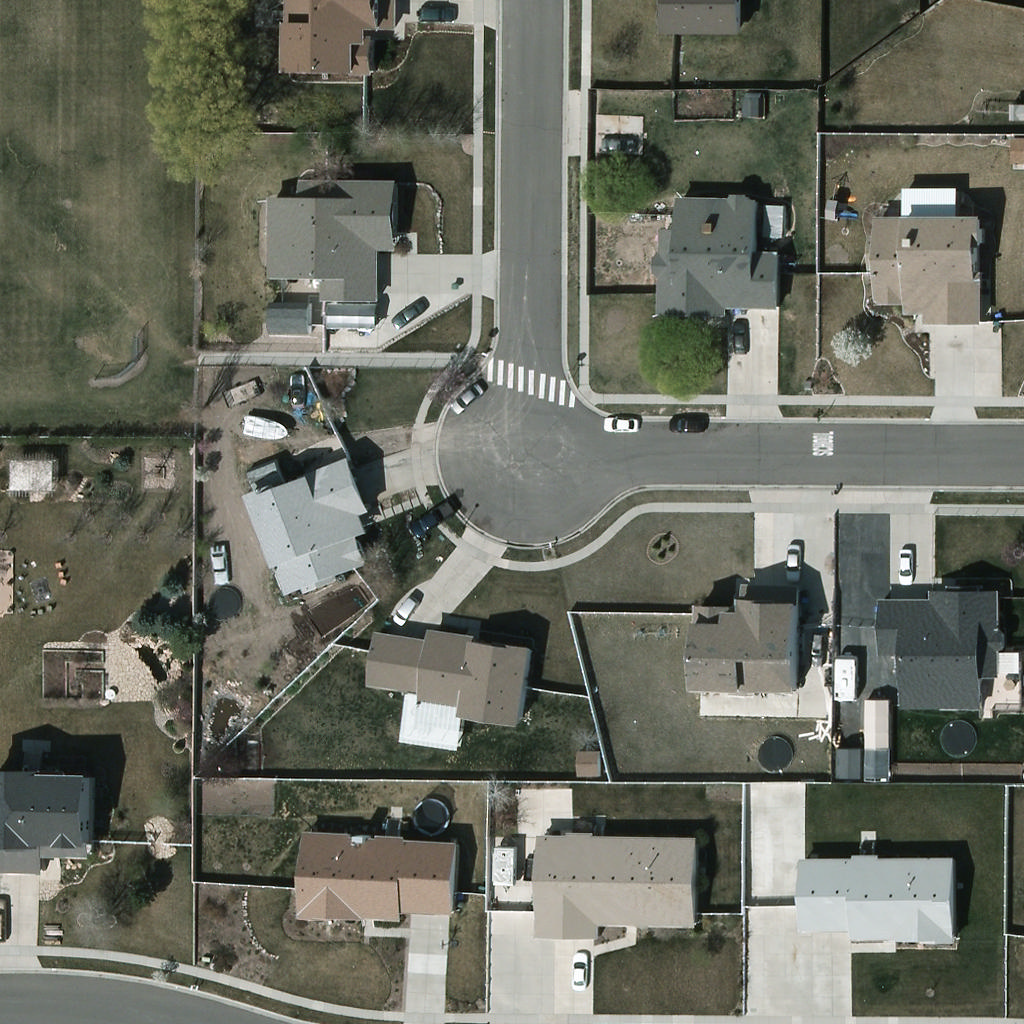
\includegraphics[width=\textwidth]{images/015Results/wrong_labels/comp_images/00000034_co.png} % Bildpfad zum ersten Bild
        \caption{\Acrlong{GT} } % Unterschrift für das erste Bild
        \label{fig:cm_trgbir} % Label für Referenzierung von Bild 1
    \end{subfigure}
    \hfill % Fügt horizontalen Platz zwischen den Subfiguren ein
    % Zweite Subfigur
    \begin{subfigure}[b]{0.45\textwidth} % 0.48\textwidth für das zweite Bild
        \includegraphics[width=\textwidth]{images/015Results/wrong_labels/comp_images/rgbir/34.png} % Bildpfad zum zweiten Bild
        \caption{Prediction} % Unterschrift für das zweite Bild
        \label{fig:cm_irgb} % Label für Referenzierung von Bild 2
    \end{subfigure}
    \caption[Comparison \acrshort{GT} and Prediction (RGBIR, F0, Validation on Validation Dataset) of image 00000034\_co.png]{Comparison of image 00000034\_co.png shows a discrepancy between ground truth and model prediction: vehicles are recognisable in the GT but not annotated, while the model (RGBIR, F0, (Validation on Validation)) detects and classifies them correctly. This calls into question the validity of GT-based metrics for distinguishing between background and object (Own representation).} % Gemeinsame Unterschrift für beide Bilder
    \label{fig:wrong_labels} % Label für die gesamte Figure-Umgebung
\end{figure}


\begin{table}[h]
\centering
\begin{tabular}{c c}
\hline
\textbf{Difference (in \% from reference)} & \textbf{Category} \\ \hline
0 -- 5 \%   & low \\ 
5 -- 10 \%  & moderate \\ 
10 -- 20 \% & high \\ 
> 20 \%     & very high \\ \hline
\end{tabular}
\caption{Classification of differences relative to the reference}
\label{tab:diff_cat}
\end{table}

\begin{figure}[htbp]
    \centering
    % Erste Spalte
    \begin{subfigure}{0.48\textwidth}
        \centering
        \includesvg[width=\linewidth]{images/015Results/02perm_exp/confusion_matrices/Difference_Matrices/RGBIR_F2_vs_RGBNDVI_F2.svg}
        \caption{RGBNDVI (F2)}
        \label{fig:perm_exp_diffM_rgbndvi_f2}
    \end{subfigure}
    \begin{subfigure}{0.48\textwidth}
        \centering
        \includesvg[width=\linewidth]{images/015Results/02perm_exp/confusion_matrices/Difference_Matrices/RGBIR_F2_vs_GBNDVI_F2.svg}
        \caption{GBNDVI (F2)}
        \label{fig:perm_exp_diffM_gbndvi_f2}
    \end{subfigure}
    
    \begin{subfigure}{0.48\textwidth}
        \centering
        \includesvg[width=\linewidth]{images/015Results/02perm_exp/confusion_matrices/Difference_Matrices/RGBIR_F2_vs_IRGB_F3.svg}
        \caption{IRGB (F3)}
        \label{fig:perm_exp_diffM_irgb_f3}
    \end{subfigure}
    \begin{subfigure}{0.48\textwidth}
        \centering
        \includesvg[width=\linewidth]{images/015Results/02perm_exp/confusion_matrices/Difference_Matrices/RGBIR_F2_vs_RIRB_F2.svg}
        \caption{RIRB (F2)}
        \label{fig:perm_exp_diffM_RIRB_f2}
    \end{subfigure}
    
    \begin{subfigure}{0.48\textwidth}
        \centering
        \includesvg[width=\linewidth]{images/015Results/02perm_exp/confusion_matrices/Difference_Matrices/RGBIR_F2_vs_RGB_F2.svg}
        \caption{RGB (F2)}
        \label{fig:perm_exp_diffM_RGB_f2}
    \end{subfigure}
    \begin{subfigure}{0.48\textwidth}
        \centering
        \includesvg[width=\linewidth]{images/015Results/02perm_exp/confusion_matrices/Difference_Matrices/RGBIR_F2_vs_RGIR_F3.svg}
        \caption{RGIR (F3)}
        \label{fig:perm_exp_diffM_RGIR_f3}
    \end{subfigure}

    \caption[Difference Matrices compared to RGBIR (Fold 2)]{Difference Matrices for all models compared against RGBIR (Fold 2). Red indicates better performance for RGBIR, blue for the respective comparison model. All values falling within the interval [–0.05, 0.05] are excluded from the matrices. Clear differences exist between channel permutations. \textit{Ship} and \textit{Tractor} are best recognised by RGBIR, while RGIR shows minimal differences. Object-background distinction remains challenging for all models, with RGIR yielding the most stable results (own representation).}
    \label{fig:perm_exp_diffM_all}
\end{figure}
\todo{Beschreibung Figures länger machen, mehr Analyse weniger "was sieht man"}



Figure~\ref{fig:perm_exp_diffM_rgbndvi_f2} illustrates clear differences in favour of RGBIR. This is particularly evident in the correct recognition of \textit{Ship} (+24~\%), \textit{Vehicle} (+16~\%), \textit{Plane} (+12~\%) and \textit{Tractor} (10~\%). There are also differences of more than 10\% in cases of confusion between \textit{Van} and \textit{Car}. In contrast, RGBNDVI has fewer misclassifications, for example in the case of \textit{Plane} (-12\%) and \textit{Van} (-23\%), which are less frequently misidentified as \textit{Background}. Overall, RGBIR shows five classes (\textit{Ship}, \textit{Tractor}, \textit{Vehicle}, \textit{Van}, \textit{Plane}) in which it performs at least 5\% better, while RGBNDVI does not show any higher classification accuracy.


Figure~\ref{fig:perm_exp_diffM_gbndvi_f2} shows a very large difference in the \textit{Tractor} class, where RGBIR is clearly superior (+22\%). In contrast, the improvement for \textit{Ship} is only +8\%. It is striking that \textit{Tractor} (-15\%), \textit{Ship} (-12\%) and \textit{Van} (-11\%) are less frequently misclassified as \textit{Background} in the GBNDVI model. Overall, RGBIR is at least 5\% better in four classes (\textit{Ship}, \textit{Tractor}, \textit{Van}, \textit{Vehicle}), while GBNDVI does not show higher accuracy in any class.




As Figure~\ref{fig:perm_exp_diffM_irgb_f3} shows, \textit{Ship} remains a class in which RGBIR is particularly strong (+21~\%). Nevertheless, misclassifications occur in both models, such as the confusion of \textit{Ship} with \textit{Camping Car} (-14\%) or \textit {Background} (-12\%). Overall, RGBIR is at least 5\% better in three classes (\textit{Ship}, \textit{Camping Car}, \textit{Vehicle}), while IRGB does not show higher accuracy in any class.




Figure~\ref{fig:perm_exp_diffM_RIRB_f2} shows a mixed picture: RGBIR has advantages in distinguishing object/background with the classes vehicle and camping car, while RIRB achieves a moderate improvement in background/object distinction (6\%) for camping cars. Noteworthy are the less frequent misclassifications in the RIRB model, where \textit{Van} (21\%) and \textit{Ship} (12\%) are not recognised as \textit{Background}. Overall, RGBIR is better in two classes (\textit{Ship}, \textit{Van}), while RIRB has higher accuracy in one class (\textit{Camping Car}).




Figure~\ref{fig:perm_exp_diffM_RGB_f2} shows clear differences in favour of the RGBIR model in the classes \textit{Ship} (12~\%) and \textit{Vehicle} (15~\%). Nevertheless, moderate misclassifications also occur here, such as the confusion of \textit{Pick Up} with \textit{Car} (6~\%) or \textit{Van} with \textit{Pick Up} (6~\%). While RGB misclassifies \textit{Vehicle} (15\%) and \textit{Ship} (10\%) less frequently than \textit{Background}, RGBIR more frequently misclassifies \textit{Background} as \textit{Pick Up} (7\%). Overall, RGBIR is superior in two classes (\textit{Ship}, \textit{Vehicle}).



The last comparison in Figure~\ref{fig:perm_exp_diffM_RGIR_f3} between RGBIR and RGIR (Fold~3) shows an almost equal result. While RGBIR confuses \textit{Van} with \textit{Car} more often (12\%) and classifies \textit{Camping Car} more often than \textit{Background} (10\%), RGIR performs moderately better for \textit{Ship} (6\%) and \textit{Van} (8\%). Overall, both models show comparable performance, with neither achieving higher classification accuracy for any one class.

Figure \ref{fig:perm_exp_example_pics} illustrates the recognition performance of the different models for the classes present in the \acrshort{VEDAI} dataset. The outstanding classification performance of all models for the \textit{Car} class is particularly evident. The situation is similar for the \textit{Truck} class, although in the example shown, the IRGB model sometimes classifies the objects as both \textit{Truck} and \textit{Vehicle}. The models also show very good results for the classes \textit{Camping Car}, \textit{Tractor}, \textit{Plane}, \textit{Pick Up} and \textit{Van}, although the GBNDVI model confuses \textit{Van} with \textit{Car}, albeit with low confidence. The class \textit{Ship} is misclassified by almost all models as \textit{Camping Car} with low confidence; RGBIR and IRGB also double-classify it as \textit{Ship} and \textit{Camping Car}. Only the RGBNDVI model correctly recognises \textit{Ship}. It is striking that the class \textit{Vehicle} is not reliably recognised by any of the models.


\begin{figure}[h!]
\centering
\renewcommand{\arraystretch}{1.2} % mehr Platz zwischen Zeilen
\setlength{\tabcolsep}{2pt} % weniger Platz zwischen Spalten
\begin{tabularx}{\textwidth}{c|*{9}{X}}
    & \textbf{Car}
    & \textbf{Truck}
    & \textbf{Camping Car}
    & \textbf{Tractor}
    & \textbf{Plane}
    & \textbf{Ship}
    & \textbf{Vehicle}
    & \textbf{Pick-Up}
    & \textbf{Van} \\ \hline
    \rotatebox{90}{\textbf{\acrshort{GT} (\acrshort{abb})}} 
    %Car
    & \includegraphics[trim={880pt 630pt 70pt 330pt},clip,width=\linewidth]{images/015Results/01abb_vs_obb/comp_images/ground_truth_abb/523.png}
    %Truck
    & \includegraphics[trim={360pt 200pt 540pt 715pt},clip,width=\linewidth]{images/015Results/01abb_vs_obb/comp_images/ground_truth_abb/212.png}
    %Camping Car
    & \includegraphics[trim={730pt 220pt 200pt 720pt},clip,width=\linewidth]{images/015Results/01abb_vs_obb/comp_images/ground_truth_abb/523.png}
    %Tractor
    & \includegraphics[trim={850pt 110pt 80pt 830pt},clip,width=\linewidth]{images/015Results/01abb_vs_obb/comp_images/ground_truth_abb/523.png}
    %Plane
    &  \includegraphics[trim={650pt 120pt 170pt 720pt},clip,width=\linewidth]{images/015Results/01abb_vs_obb/comp_images/ground_truth_abb/487.png}
    %Ship
    & \includegraphics[trim={230pt 200pt 680pt 725pt},clip,width=\linewidth]{images/015Results/01abb_vs_obb/comp_images/ground_truth_abb/509.png}
    %vehicle
    & \includegraphics[trim={440pt 360pt 460pt 555pt},clip,width=\linewidth]{images/015Results/01abb_vs_obb/comp_images/ground_truth_abb/427.png}
    %Pick Up
    & \includegraphics[trim={740pt 420pt 180pt 510pt},clip,width=\linewidth]{images/015Results/01abb_vs_obb/comp_images/ground_truth_abb/523.png}
    %Van
    & \includegraphics[trim={300pt 355pt 610pt 570pt},clip,width=\linewidth]{images/015Results/01abb_vs_obb/comp_images/ground_truth_abb/198.png} \\ \hline

    \rotatebox{90}{\textbf{\acrshort{GT} (\acrshort{obb})}} 
    %Car
    & \includegraphics[trim={880pt 630pt 70pt 330pt},clip,width=\linewidth]{images/015Results/01abb_vs_obb/comp_images/ground_truth_obb/523.png}
    %Truck
    & \includegraphics[trim={360pt 200pt 540pt 715pt},clip,width=\linewidth]{images/015Results/01abb_vs_obb/comp_images/ground_truth_obb/212.png}
    %Camping Car
    & \includegraphics[trim={730pt 220pt 200pt 720pt},clip,width=\linewidth]{images/015Results/01abb_vs_obb/comp_images/ground_truth_obb/523.png}
    %Tractor
    & \includegraphics[trim={850pt 110pt 80pt 830pt},clip,width=\linewidth]{images/015Results/01abb_vs_obb/comp_images/ground_truth_obb/523.png}
    %Plane
    &  \includegraphics[trim={650pt 120pt 170pt 720pt},clip,width=\linewidth]{images/015Results/01abb_vs_obb/comp_images/ground_truth_obb/487.png}
    %Ship
    & \includegraphics[trim={230pt 200pt 680pt 725pt},clip,width=\linewidth]{images/015Results/01abb_vs_obb/comp_images/ground_truth_obb/509.png}
    %vehicle
    & \includegraphics[trim={440pt 360pt 460pt 555pt},clip,width=\linewidth]{images/015Results/01abb_vs_obb/comp_images/ground_truth_obb/427.png}
    %Pick Up
    & \includegraphics[trim={740pt 420pt 180pt 510pt},clip,width=\linewidth]{images/015Results/01abb_vs_obb/comp_images/ground_truth_obb/523.png}
    %Van
    & \includegraphics[trim={300pt 355pt 610pt 570pt},clip,width=\linewidth]{images/015Results/01abb_vs_obb/comp_images/ground_truth_obb/198.png} \\ \hline
    \rotatebox{90}{\textbf{\acrshort{abb}}} 
    %Car
    & \includegraphics[trim={880pt 630pt 70pt 330pt},clip,width=\linewidth]{images/015Results/01abb_vs_obb/comp_images/abb/523.png}
    %Truck
    & \includegraphics[trim={360pt 200pt 540pt 715pt},clip,width=\linewidth]{images/015Results/01abb_vs_obb/comp_images/abb/212.png}
    %Camping Car
    & \includegraphics[trim={730pt 220pt 200pt 720pt},clip,width=\linewidth]{images/015Results/01abb_vs_obb/comp_images/abb/523.png}
    %Tractor
    & \includegraphics[trim={850pt 110pt 80pt 830pt},clip,width=\linewidth]{images/015Results/01abb_vs_obb/comp_images/abb/523.png}
    %Plane
    &  \includegraphics[trim={650pt 120pt 170pt 720pt},clip,width=\linewidth]{images/015Results/01abb_vs_obb/comp_images/abb/487.png}
    %Ship
    & \includegraphics[trim={230pt 200pt 680pt 725pt},clip,width=\linewidth]{images/015Results/01abb_vs_obb/comp_images/abb/509.png}
    %vehicle
    & \includegraphics[trim={440pt 360pt 460pt 555pt},clip,width=\linewidth]{images/015Results/01abb_vs_obb/comp_images/abb/427.png}
    %Pick Up
    & \includegraphics[trim={740pt 420pt 180pt 510pt},clip,width=\linewidth]{images/015Results/01abb_vs_obb/comp_images/abb/523.png}
    %Van
    & \includegraphics[trim={300pt 355pt 610pt 570pt},clip,width=\linewidth]{images/015Results/01abb_vs_obb/comp_images/abb/198.png} \\ \hline
    \rotatebox{90}{\textbf{\acrshort{obb}}} 
    %Car
    & \includegraphics[trim={880pt 630pt 70pt 330pt},clip,width=\linewidth]{images/015Results/01abb_vs_obb/comp_images/obb/523.png}
    %Truck
    & \includegraphics[trim={360pt 200pt 540pt 715pt},clip,width=\linewidth]{images/015Results/01abb_vs_obb/comp_images/obb/212.png}
    %Camping Car
    & \includegraphics[trim={730pt 220pt 200pt 720pt},clip,width=\linewidth]{images/015Results/01abb_vs_obb/comp_images/obb/523.png}
    %Tractor
    & \includegraphics[trim={850pt 110pt 80pt 830pt},clip,width=\linewidth]{images/015Results/01abb_vs_obb/comp_images/obb/523.png}
    %Plane
    &  \includegraphics[trim={650pt 120pt 170pt 720pt},clip,width=\linewidth]{images/015Results/01abb_vs_obb/comp_images/obb/487.png}
    %Ship
    & \includegraphics[trim={230pt 200pt 680pt 725pt},clip,width=\linewidth]{images/015Results/01abb_vs_obb/comp_images/obb/509.png}
    %vehicle
    & \includegraphics[trim={440pt 360pt 460pt 555pt},clip,width=\linewidth]{images/015Results/01abb_vs_obb/comp_images/obb/427.png}
    %Pick Up
    & \includegraphics[trim={740pt 420pt 180pt 510pt},clip,width=\linewidth]{images/015Results/01abb_vs_obb/comp_images/obb/523.png}
    %Van
    & \includegraphics[trim={300pt 355pt 610pt 570pt},clip,width=\linewidth]{images/015Results/01abb_vs_obb/comp_images/obb/198.png} \\ \hline
     \rotatebox{90}{\textbf{\acrshort{abb} in \acrshort{obb}}} 
    %Car
    & \includegraphics[trim={880pt 630pt 70pt 330pt},clip,width=\linewidth]{images/015Results/01abb_vs_obb/comp_images/aab_old/523.png}
    %Truck
    & \includegraphics[trim={360pt 200pt 540pt 715pt},clip,width=\linewidth]{images/015Results/01abb_vs_obb/comp_images/aab_old/212.png}
    %Camping Car
    & \includegraphics[trim={730pt 220pt 200pt 720pt},clip,width=\linewidth]{images/015Results/01abb_vs_obb/comp_images/aab_old/523.png}
    %Tractor
    & \includegraphics[trim={850pt 110pt 80pt 830pt},clip,width=\linewidth]{images/015Results/01abb_vs_obb/comp_images/aab_old/523.png}
    %Plane
    &  \includegraphics[trim={650pt 120pt 170pt 720pt},clip,width=\linewidth]{images/015Results/01abb_vs_obb/comp_images/aab_old/487.png}
    %Ship
    & \includegraphics[trim={230pt 200pt 680pt 725pt},clip,width=\linewidth]{images/015Results/01abb_vs_obb/comp_images/aab_old/509.png}
    %vehicle
    & \includegraphics[trim={440pt 360pt 460pt 555pt},clip,width=\linewidth]{images/015Results/01abb_vs_obb/comp_images/aab_old/427.png}
    %Pick Up
    & \includegraphics[trim={740pt 420pt 180pt 510pt},clip,width=\linewidth]{images/015Results/01abb_vs_obb/comp_images/aab_old/523.png}
    %Van
    & \includegraphics[trim={300pt 355pt 610pt 570pt},clip,width=\linewidth]{images/015Results/01abb_vs_obb/comp_images/aab_old/198.png} \\ \hline
\end{tabularx}
\caption[aab and obb: Examples of different classes for the object recognition performance]{Examples of different classes for the object recognition performance of different bounding box formats. The numbers displayed on the bounding boxes indicate the confidence of the model in the classification of the respective box. For Color Scheme explanation see Tab. \ref{tab:class_colors}}.
\label{fig:aab_obb_example_pics}
\end{figure}
\FloatBarrier






%##########################################################################
%##########################################################################
%##########################################################################
%##########################################################################
%##########################################################################
%##########################################################################
%##########################################################################
%##########################################################################
%##########################################################################
\section{Ablation Studies}

The box plots in Fig. \ref{fig:ablation_map50-95:val_on_test} of the 6-fold cross-validation show that the models for the red, green, blue and IR channels are in the range of \acrshort{mAP}@0.5--0.95 = 0.52–0.54 on the test data set. A single value in the IR model reaches 0.5777, but this is well outside the central range of the other folds and should be interpreted as an outlier. Overall, no significant differences can be observed between the Red, Green, Blue and IR models, while NDVI performs significantly worse with a median of around 0.44. Similar results can be seen in Fig. \ref{fig:ablation_map50-95:val_on_val} for the performance on the validation data.

The evaluation of the results in Tab. \ref{tab:ablation_best_folds_test} also shows that fold 4 and fold 2 in particular achieved the best results on the validation data set. On the test data set, however, folds 0, 2 and 3 achieve the best performance.  

Overall, the IR model shows the highest performance and achieves the highest \acrshort{mAP} value compared to the other variants examined.




\begin{figure}[htbp]
    \centering
    \includesvg[width=0.8\textwidth]{images/015Results/03ablation/best_val_on_test.svg}
    \caption[Comparison of \acrshort{mAP}@0.5--0.95 values for channels: red, green, blue, ndvi (Best validation model on test dataset)]{Comparison of \acrshort{mAP}@0.5--0.95 values for channels: Red, Green, Blue, NDVI (Best validation model on test dataset). The red dot is the fold, that has the best \acrshort{mAP}@0.5--0.95 at the validation dataset (see fig. \ref{fig:ablation_map50-95:val_on_val}). Minimal fluctuations in quantiles between individual channels indicate that a single channel is fundamentally suitable for object recognition, but that significantly better results can be achieved in combination with other channels. The grey value gradients of the individual channels are similar (with the exception of NDVI), although models with NDVI perform significantly worse, presumably due to greater gradations in the grey values (Own representation).}
    \label{fig:ablation_map50-95:val_on_test}
\end{figure}


\begin{figure}[htbp]
    \centering
    \includesvg[width=0.8\textwidth]{images/015Results/03ablation/best_val_on_val.svg}
    \caption[Comparison of \acrshort{mAP}@0.5--0.95 values for channels: red, green, blue, ndvi (Best validation model on validation dataset)]{Comparison of \acrshort{mAP}@0.5--0.95 values for channels: Red, Green, Blue, NDVI (Best validation model on validation dataset). The quantile fluctuations of the R, G and B channels are very low, as the visible spectral colours probably contain similar information individually. The IR channel shows significantly broader quantiles, presumably due to stronger grey value fluctuations. NDVI perform significantly worse due to the pronounced gradations in the grey values. (Own representation)}
    \label{fig:ablation_map50-95:val_on_val}
\end{figure}

\begin{figure}[htbp]
    \centering
    % Erste Spalte
       
    \begin{subfigure}{0.48\textwidth}
        \centering
        \includesvg[width=\linewidth]{images/015Results/03ablation/conf_matr_ir_f0.svg}
        \caption{IR (F3)}
        \label{fig:ablation_confM_IR_f0}
    \end{subfigure}

    \begin{subfigure}{0.48\textwidth}
        \centering
        \includesvg[width=\linewidth]{images/015Results/03ablation/diff_matric/IR_F0_vs_R_F2.svg}
        \caption{Red (F2)}
        \label{fig:ablation_diffM_r_f2}
    \end{subfigure}
    \begin{subfigure}{0.48\textwidth}
        \centering
        \includesvg[width=\linewidth]{images/015Results/03ablation/diff_matric/IR_F0_vs_G_F3.svg}
        \caption{Green (F3)}
        \label{fig:ablation_diffM_g_f3}
    \end{subfigure}
    
    \begin{subfigure}{0.48\textwidth}
        \centering
        \includesvg[width=\linewidth]{images/015Results/03ablation/diff_matric/IR_F0_vs_B_F2.svg}
        \caption{Blue (F2)}
        \label{fig:ablation_diffM_b_f2}
    \end{subfigure}
    \begin{subfigure}{0.48\textwidth}
        \centering
        \includesvg[width=\linewidth]{images/015Results/03ablation/diff_matric/IR_F0_vs_NDVI_F0.svg}
        \caption{NDVI (F0)}
        \label{fig:ablation_diffM_NDVI_f0}
    \end{subfigure}
    \caption[Confusion Matrix for IR Model at Fold 3 and the Difference Matrices compared to this Model]{Confusion Matrix for IR Model at Fold 3 and the Difference Matrices compared to this Model. Red indicates better performance for IR, blue for the respective comparison model. All values falling within the interval [–0.05, 0.05] are excluded from the matrices. IR generally outperforms other channels, indicating that its additional spectral information improves feature discrimination. High performance for \textit{Car}, \textit{Tractor}, and \textit{Pick Up} reflects the influence of abundant training data, while persistent confusion for the generic \textit{Vehicle} class highlights limitations in distinguishing objects without distinctive shape or spectral cues (own representation).
}
    \label{fig:ablation_diffM_all}
\end{figure}

\FloatBarrier
\subsection*{Comparison with Confusion Matrices}
\label{subsec:ablation_comp_confusion_matric}

Following the analysis of the permutation experiments (see Section \ref{subsec:permexp_comp_confusion_matric}), the classification performance of the models is now examined using the confusion matrix of the IR model as a reference (see Figure \ref{fig:ablation_confM_IR_f0}). The evaluation is carried out in the same way as the categorisation of the differences in Table \ref{tab:diff_cat}.  

The IR model shows a perfect recognition rate of 100\,\% for the class \textit{Plane}. Very high recognition rates of over 80\,\% were also achieved for the classes \textit{Car} and \textit{Tractor}.

Good performance with recognition rates between 60\,\% and 80\,\% was achieved for the classes \textit{Truck}, \textit{Ship}, \textit{Camping Car} and \textit{Pick Up}. In contrast, the recognition rates for the classes \textit{Van} and \textit{Vehicle} are in the range of 40–60\%, which represents only moderate classification performance. 

Particularly striking is the incorrect classification of the class \textit{Vehicle}, which was assigned to \textit{Background} in 45\% of cases. In addition, increased misclassifications occur in several other categories: \textit{Pick Up} (17\%), \textit{Ship} (18\%), \textit{Camping Car} (28\%) and \textit{Van} (39\%) have particularly high rates of misclassification. These results highlight the specific weaknesses of the IR model compared to the variants examined in the permutation experiments.
  


The analysis of the difference matrices illustrates the respective performance of individual channels in comparison to the IR reference model (see Figure \ref{fig:ablation_confM_IR_f0}).

Figure \ref{fig:ablation_diffM_r_f2} shows that IR performs significantly better at recognising the \textit{Vehicle} class compared to the red channel alone (15\%). For the \textit{Van} class, however, the red channel proves to be advantageous, as it achieves a 16\,\% higher recognition rate here. The IR model, on the other hand, shows advantages in distinguishing object/\textit{Background} from \textit{Van} (12\,\%), \textit{Camping Car} (9\,\%) and, to a moderate extent, \textit{Pick Up} (6\,\%).
    
Figure \ref{fig:ablation_diffM_g_f3} shows the comparison with the green channel. Here, the green channel achieves significantly higher performance in the detection of \textit{Ship} (26\,\%) and a high improvement in \textit{Van} (17\,\%). The IR model, on the other hand, is superior in the detection of \textit{Truck} (14\,\%). Particularly striking is the distinction between objects and the background: here, IR performs significantly better with \textit{Van} at 24\,\%. IR also achieves high precision for \textit{Ship} and \textit{Vehicle}, while there are moderate advantages in distinguishing object/\textit{Background} for \textit{Camping Car} (8\,\%) and \textit{Pick Up} (6\,\%). In contrast, the green channel shows better results for \textit{Truck} (15\,\%) and moderate results for \textit{Tractor} (6\,\%). There is no significant difference in the \textit{Car} class. Overall, IR is at least 5\,\% better in two classes (\textit{Truck}, \textit{Tractor}), while the green channel has advantages in three other classes (\textit{Van}, \textit{Camping Car}, \textit{Pick Up}).

Figure \ref{fig:ablation_diffM_b_f2} shows the comparison with the blue channel. This shows moderate advantages for \textit{Camping Car} (6\,\%) and \textit{Pick Up} (6\,\%) as well as a significant improvement for \textit{Van} (13\,\%). The IR model, on the other hand, is superior for \textit{Truck} (10\,\%) and moderately superior for \textit{Ship} (7\,\%) and \textit{Vehicle} (9\,\%). In addition, IR is better at distinguishing \textit{Van} from \textit{Background} (10\,\%) and achieves moderate advantages in this distinction for \textit{Camping Car} (6\,\%) and \textit{Pick Up} (5\,\%). The blue channel, on the other hand, shows moderate improvements in distinguishing \textit{Truck} (8\,\%) and \textit{Vehicle} (5\,\%) from the \textit{Background}. Overall, IR is clearly superior in three classes (\textit{Camping Car}, \textit{Van}, \textit{Pick Up}), while the blue channel has advantages in two classes (\textit{Truck}, \textit{Vehicle}).  

Compared to NDVI, IR shows higher precision for the classes \textit{Car} (10\,\%), \textit{Truck} (12\,\%), \textit{Tractor} (16\,\%) and \textit{Camping Car} (14\,\%) classes and is significantly more accurate for \textit{Ship} (24\,\%) in particular. IR also achieves a moderate improvement (6\,\%) for \textit{Vehicle}. NDVI, on the other hand, shows advantages in distinguishing between background and object, particularly moderately for \textit{Truck} (9\,\%) and \textit{Camping Car} (7\,\%), as well as higher precision for \textit{Ship} (26\,\%) and \textit{Tractor} (13\,\%). Overall, IR is at least 5\% better than NDVI in six classes (\textit{Car}, \textit{Truck}, \textit{Ship}, \textit{Tractor}, \textit{Camping Car}, \textit{Vehicle}), while NDVI only shows advantages in distinguishing between object and Background in four cases. 

In summary, it can be said that all models – with the exception of the NDVI model – demonstrate high classification performance in the \textit{Car} category, which is also clearly reflected in the example images (see Figure \ref{fig:ablation_example_pics}). At the same time, both the difference matrices and the example images show that misclassifications between background and object continue to occur to a considerable extent, especially within the \textit{Vehicle} class (see Confusion Matrix \ref{fig:ablation_confM_IR_f0}). What is striking here is the IR channel, which shows a particularly high confusion rate between objects and background in the examples shown in Figure \ref{fig:ablation_example_pics}, while in the other channels, more objects are correctly recognised overall. Furthermore, the confusion of the class \textit{Van} with \textit{Car} in the Red model is confirmed in the difference matrix \ref{fig:ablation_diffM_g_f3}. Compared to the reference model (6\%, see Figure \ref{fig:ablation_confM_IR_f0}), this confusion rate does not indicate either an improvement or a deterioration in performance. The NDVI model, on the other hand, shows a significantly reduced performance: Figure \ref{fig:ablation_example_pics} shows that, with the exception of the correct classification of \textit{Van} and the misclassification of \textit{Truck} as \textit{Vehicle}, no accurate results were achieved. All other classes were incorrectly assigned to the background.






\begin{table}[h]
\centering
\begin{tabular}{l c c}
\hline
\textbf{Channel} & \textbf{Best mAP Fold (Validation)} & \textbf{Best mAP Fold (Test)} \\ 
\hline
Red   & 4 & 2 (0.5408) \\
Green & 4 & 3 (0.5449) \\
Blue  & 4 & 2 (0.5449) \\
IR    & 4 & 0 (0.5777) \\
NDVI  & 2 & 0 (0.4467) \\
\hline
\end{tabular}
\caption{Best fold per model on validation and test sets, with test mAP@50-95 values}
\label{tab:ablation_best_folds_test}
\end{table}

\begin{figure}[h!]
\centering
\renewcommand{\arraystretch}{1.2} % mehr Platz zwischen Zeilen
\setlength{\tabcolsep}{2pt} % weniger Platz zwischen Spalten
\begin{tabularx}{\textwidth}{c|*{9}{X}}
    & \textbf{Car}
    & \textbf{Truck}
    & \textbf{Camping Car}
    & \textbf{Tractor}
    & \textbf{Plane}
    & \textbf{Ship}
    & \textbf{Vehicle}
    & \textbf{Pick-Up}
    & \textbf{Van} \\ \hline
    \rotatebox{90}{\textbf{\acrshort{GT} (\acrshort{abb})}} 
    %Car
    & \includegraphics[trim={880pt 630pt 70pt 330pt},clip,width=\linewidth]{images/015Results/01abb_vs_obb/comp_images/ground_truth_abb/523.png}
    %Truck
    & \includegraphics[trim={360pt 200pt 540pt 715pt},clip,width=\linewidth]{images/015Results/01abb_vs_obb/comp_images/ground_truth_abb/212.png}
    %Camping Car
    & \includegraphics[trim={730pt 220pt 200pt 720pt},clip,width=\linewidth]{images/015Results/01abb_vs_obb/comp_images/ground_truth_abb/523.png}
    %Tractor
    & \includegraphics[trim={850pt 110pt 80pt 830pt},clip,width=\linewidth]{images/015Results/01abb_vs_obb/comp_images/ground_truth_abb/523.png}
    %Plane
    &  \includegraphics[trim={650pt 120pt 170pt 720pt},clip,width=\linewidth]{images/015Results/01abb_vs_obb/comp_images/ground_truth_abb/487.png}
    %Ship
    & \includegraphics[trim={230pt 200pt 680pt 725pt},clip,width=\linewidth]{images/015Results/01abb_vs_obb/comp_images/ground_truth_abb/509.png}
    %vehicle
    & \includegraphics[trim={440pt 360pt 460pt 555pt},clip,width=\linewidth]{images/015Results/01abb_vs_obb/comp_images/ground_truth_abb/427.png}
    %Pick Up
    & \includegraphics[trim={740pt 420pt 180pt 510pt},clip,width=\linewidth]{images/015Results/01abb_vs_obb/comp_images/ground_truth_abb/523.png}
    %Van
    & \includegraphics[trim={300pt 355pt 610pt 570pt},clip,width=\linewidth]{images/015Results/01abb_vs_obb/comp_images/ground_truth_abb/198.png} \\ \hline

    \rotatebox{90}{\textbf{\acrshort{GT} (\acrshort{obb})}} 
    %Car
    & \includegraphics[trim={880pt 630pt 70pt 330pt},clip,width=\linewidth]{images/015Results/01abb_vs_obb/comp_images/ground_truth_obb/523.png}
    %Truck
    & \includegraphics[trim={360pt 200pt 540pt 715pt},clip,width=\linewidth]{images/015Results/01abb_vs_obb/comp_images/ground_truth_obb/212.png}
    %Camping Car
    & \includegraphics[trim={730pt 220pt 200pt 720pt},clip,width=\linewidth]{images/015Results/01abb_vs_obb/comp_images/ground_truth_obb/523.png}
    %Tractor
    & \includegraphics[trim={850pt 110pt 80pt 830pt},clip,width=\linewidth]{images/015Results/01abb_vs_obb/comp_images/ground_truth_obb/523.png}
    %Plane
    &  \includegraphics[trim={650pt 120pt 170pt 720pt},clip,width=\linewidth]{images/015Results/01abb_vs_obb/comp_images/ground_truth_obb/487.png}
    %Ship
    & \includegraphics[trim={230pt 200pt 680pt 725pt},clip,width=\linewidth]{images/015Results/01abb_vs_obb/comp_images/ground_truth_obb/509.png}
    %vehicle
    & \includegraphics[trim={440pt 360pt 460pt 555pt},clip,width=\linewidth]{images/015Results/01abb_vs_obb/comp_images/ground_truth_obb/427.png}
    %Pick Up
    & \includegraphics[trim={740pt 420pt 180pt 510pt},clip,width=\linewidth]{images/015Results/01abb_vs_obb/comp_images/ground_truth_obb/523.png}
    %Van
    & \includegraphics[trim={300pt 355pt 610pt 570pt},clip,width=\linewidth]{images/015Results/01abb_vs_obb/comp_images/ground_truth_obb/198.png} \\ \hline
    \rotatebox{90}{\textbf{\acrshort{abb}}} 
    %Car
    & \includegraphics[trim={880pt 630pt 70pt 330pt},clip,width=\linewidth]{images/015Results/01abb_vs_obb/comp_images/abb/523.png}
    %Truck
    & \includegraphics[trim={360pt 200pt 540pt 715pt},clip,width=\linewidth]{images/015Results/01abb_vs_obb/comp_images/abb/212.png}
    %Camping Car
    & \includegraphics[trim={730pt 220pt 200pt 720pt},clip,width=\linewidth]{images/015Results/01abb_vs_obb/comp_images/abb/523.png}
    %Tractor
    & \includegraphics[trim={850pt 110pt 80pt 830pt},clip,width=\linewidth]{images/015Results/01abb_vs_obb/comp_images/abb/523.png}
    %Plane
    &  \includegraphics[trim={650pt 120pt 170pt 720pt},clip,width=\linewidth]{images/015Results/01abb_vs_obb/comp_images/abb/487.png}
    %Ship
    & \includegraphics[trim={230pt 200pt 680pt 725pt},clip,width=\linewidth]{images/015Results/01abb_vs_obb/comp_images/abb/509.png}
    %vehicle
    & \includegraphics[trim={440pt 360pt 460pt 555pt},clip,width=\linewidth]{images/015Results/01abb_vs_obb/comp_images/abb/427.png}
    %Pick Up
    & \includegraphics[trim={740pt 420pt 180pt 510pt},clip,width=\linewidth]{images/015Results/01abb_vs_obb/comp_images/abb/523.png}
    %Van
    & \includegraphics[trim={300pt 355pt 610pt 570pt},clip,width=\linewidth]{images/015Results/01abb_vs_obb/comp_images/abb/198.png} \\ \hline
    \rotatebox{90}{\textbf{\acrshort{obb}}} 
    %Car
    & \includegraphics[trim={880pt 630pt 70pt 330pt},clip,width=\linewidth]{images/015Results/01abb_vs_obb/comp_images/obb/523.png}
    %Truck
    & \includegraphics[trim={360pt 200pt 540pt 715pt},clip,width=\linewidth]{images/015Results/01abb_vs_obb/comp_images/obb/212.png}
    %Camping Car
    & \includegraphics[trim={730pt 220pt 200pt 720pt},clip,width=\linewidth]{images/015Results/01abb_vs_obb/comp_images/obb/523.png}
    %Tractor
    & \includegraphics[trim={850pt 110pt 80pt 830pt},clip,width=\linewidth]{images/015Results/01abb_vs_obb/comp_images/obb/523.png}
    %Plane
    &  \includegraphics[trim={650pt 120pt 170pt 720pt},clip,width=\linewidth]{images/015Results/01abb_vs_obb/comp_images/obb/487.png}
    %Ship
    & \includegraphics[trim={230pt 200pt 680pt 725pt},clip,width=\linewidth]{images/015Results/01abb_vs_obb/comp_images/obb/509.png}
    %vehicle
    & \includegraphics[trim={440pt 360pt 460pt 555pt},clip,width=\linewidth]{images/015Results/01abb_vs_obb/comp_images/obb/427.png}
    %Pick Up
    & \includegraphics[trim={740pt 420pt 180pt 510pt},clip,width=\linewidth]{images/015Results/01abb_vs_obb/comp_images/obb/523.png}
    %Van
    & \includegraphics[trim={300pt 355pt 610pt 570pt},clip,width=\linewidth]{images/015Results/01abb_vs_obb/comp_images/obb/198.png} \\ \hline
     \rotatebox{90}{\textbf{\acrshort{abb} in \acrshort{obb}}} 
    %Car
    & \includegraphics[trim={880pt 630pt 70pt 330pt},clip,width=\linewidth]{images/015Results/01abb_vs_obb/comp_images/aab_old/523.png}
    %Truck
    & \includegraphics[trim={360pt 200pt 540pt 715pt},clip,width=\linewidth]{images/015Results/01abb_vs_obb/comp_images/aab_old/212.png}
    %Camping Car
    & \includegraphics[trim={730pt 220pt 200pt 720pt},clip,width=\linewidth]{images/015Results/01abb_vs_obb/comp_images/aab_old/523.png}
    %Tractor
    & \includegraphics[trim={850pt 110pt 80pt 830pt},clip,width=\linewidth]{images/015Results/01abb_vs_obb/comp_images/aab_old/523.png}
    %Plane
    &  \includegraphics[trim={650pt 120pt 170pt 720pt},clip,width=\linewidth]{images/015Results/01abb_vs_obb/comp_images/aab_old/487.png}
    %Ship
    & \includegraphics[trim={230pt 200pt 680pt 725pt},clip,width=\linewidth]{images/015Results/01abb_vs_obb/comp_images/aab_old/509.png}
    %vehicle
    & \includegraphics[trim={440pt 360pt 460pt 555pt},clip,width=\linewidth]{images/015Results/01abb_vs_obb/comp_images/aab_old/427.png}
    %Pick Up
    & \includegraphics[trim={740pt 420pt 180pt 510pt},clip,width=\linewidth]{images/015Results/01abb_vs_obb/comp_images/aab_old/523.png}
    %Van
    & \includegraphics[trim={300pt 355pt 610pt 570pt},clip,width=\linewidth]{images/015Results/01abb_vs_obb/comp_images/aab_old/198.png} \\ \hline
\end{tabularx}
\caption[aab and obb: Examples of different classes for the object recognition performance]{Examples of different classes for the object recognition performance of different bounding box formats. The numbers displayed on the bounding boxes indicate the confidence of the model in the classification of the respective box. For Color Scheme explanation see Tab. \ref{tab:class_colors}}.
\label{fig:aab_obb_example_pics}
\end{figure}



